\documentclass[a4paper,12pt]{book}
\usepackage[utf8]{inputenc}
\usepackage{mathtools}

% Allow the change of line spacing
\usepackage{setspace}
\usepackage{tabularx}
\usepackage{graphicx}
\usepackage[usenames,dvipsnames,table]{xcolor}
\usepackage{minted}


%\usepackage{hyperref}
%\usepackage{breakurl}

%opening
%\title{Trainmining}
%\author{Grupo de Sistemas Inteligentes \\ Universidad Politécnica de Madrid}


\begin{document}
\newcommand\litem[1]{\item{\bfseries #1 }}
\renewcommand{\arraystretch}{1.5} %Makes tables less crammed

\newcommand\headcell[1]{%
  \multicolumn{1}{c|}{\cellcolor{MidnightBlue}\bfseries\sffamily\textcolor{white}{#1}}
}

%\renewcommand{\abstractname}{Executive Summary}
%\begin{abstract}
%
%\end{abstract}

% Set line spacing to 1.5
\onehalfspacing

%% Begin a new titlepage. Tit	lepages have special settings like the absence of page numbers.
\begin{titlepage}
\sffamily
% Set the text of the page to right-aligned until \end{flushright}
\begin{flushright}

% Set the space between right page border and text to 2.5cm
\rightskip=-1cm

% Show an image at this position

\includegraphics[scale=1]{./img/logoGSI.png} 
%\includegraphics[bb=0 0 204 110]{web40logo.png}

% Skip a little space
\bigskip
\bigskip
\bigskip



% Create a title for the document and write it in bold font
\LARGE{\textbf{Deliverable 4. Prototype Description.}}
% Again, do a line break
\linebreak
% Create a subtitle
\large{Design and implementation of a predictive module prototype.}

% Skip some space
%\bigskip
%\bigskip
%\bigskip
%\bigskip
\bigskip

% Write in very large letters
\LARGE{Grupo de Sistemas Inteligentes}
\linebreak
\large{Departamento de Ingeniería de Sistemas Telemáticos}
% Do a line break right after the \LARGE{...} text
\linebreak
% Write in large letters
\large{Universidad Politécnica de Madrid.}

% Skip some space
\bigskip
\bigskip
\bigskip
\bigskip
\bigskip
\bigskip

\large{Project Report}

% Skip some space
\bigskip

\normalsize{Madrid, February 2013}

% Skip some space
\bigskip
\bigskip
\bigskip
\bigskip
\bigskip
\bigskip
\bigskip
\bigskip
\bigskip
\bigskip
\bigskip
\bigskip
\bigskip
\bigskip
\bigskip
\bigskip

% Provide some author information
\normalsize{Authors:}
\linebreak
\large{Adrián Pérez Orozco}
\linebreak
\large{Álvaro Carrera Barroso}
\linebreak
\large{Carlos A. Iglesias Fernández}

% End right-alignment at this point
\end{flushright}
% End the title page
\end{titlepage}

%\maketitle

\pagenumbering{roman}
\section*{Executive Summary}
\addcontentsline{toc}{section}{Executive Summary} % si queremos que aparezca en el índice
This document describes the design and implementation of a prototype predictive module for Thales' railway maintenance network. This implementation relies on already existing predictive rules which have been previously obtained from data mining procedures.

The prototype provides therefore a way to apply said obtained knowledge to actual situations, evaluating the rules and determining an output for each situation. It works as a rule-engine which takes the current situation as an input and outputs a list of predicted events along with an associated confidence for each of them. The system has been implemented in the form of a Java module, and can therefore be used as a standalone system or be integrated onto larger systems at convenience. It relies on the JBoss Drools Expert library, which provides an efficient and reliable rule-engine environment.

In this document, the architecture of the implemented prototype will be explained on detail. Furthermore, performance specifications are described as a result of several testing procedures.


\newpage
\tableofcontents % indice de contenidos
\addcontentsline{toc}{section}{Contents} % para que aparezca en el indice de 
\cleardoublepage
\addcontentsline{toc}{section}{List of Figures} % para que aparezca en el indice de contenidos
\listoffigures % indice de figuras

\cleardoublepage
\addcontentsline{toc}{section}{List of tables} % para que aparezca en el indice de contenidos
\listoftables % indice de tablas
\cleardoublepage

\setcounter{page}{1}
\pagenumbering{arabic}

\chapter{Chapter 1}
\section{Introduction}
\label{sec:context}
Maintenance is one of the most important tasks to assure the quality and correct operation of any kind of system. Even the highest quality systems, built by the best engineers to operate for long periods with the least possible human assistance, will eventually be exposed to damage or malfunction. In order to avoid the negative effects that system malfunction can produce, a significant amount of resources and effort is usually needed to be put on maintenance tasks. However, putting resources and effort on maintenance procedures might still not be enough if the procedures and strategies are not adequate and efficient.

Traditionally, we have discerned between two types of maintenance procedures:
\begin{itemize}
\item \emph{Corrective maintenance} is the most common approach, although it has very important limitations. With this approach, elements of our system are repaired or replaced once they have failed or worn out, to bring them back to operation. This usually means a high downtime in operation, as no actions are taken until our system is already malfunctioning.

\item \emph{Preventive maintenance} focuses on preventing these failures. Elements can be periodically examined and analysed in order to control their operation and perform simpler procedures to adjust them before reaching malfunction and downtime. This approach means much higher costs, as a significantly bigger amount of time is needed to monitor the elements on our system and correct them. However, as downtime means business losses in almost all cases, these higher costs usually pay back in terms of loss reduction.
\end{itemize}

A balance can be easily achieved by spending on preventive maintenance not more than the losses we would suffer from downtime if we were using a corrective approach.

However, the costs of preventive maintenance can be drastically reduced by optimising procedures and using the adequate techniques. For example, we can reduce the amount of variables and magnitudes we are monitoring (and which cost us money to monitor) if we know which ones give the better insight on the status on our systems. The same can be done with corrective maintenance. If we can somehow foresee which systems are going to fail, we can be prepared and reduce impact on our business even if we cannot do anything to prevent its failure.

In both cases, \emph{prediction} can be a key element for maintenance optimisation. Either we know which are the indicators of a system deterioration which we can repair, or we know which systems are going to fail and when to be prepared and optimise corrective procedures. We can even speak of a new type of maintenance - \emph{predictive maintenance} - which embraces several techniques to try and obtain this knowledge of future events.

\section{Project overview}
The project \emph{Trainmining} aims to design predictive maintenance techniques on already-existing maintenance stations of a railway network. These maintenance stations monitor different elements and subsystems over a railway line and raises alarms whenever a line element fails or requires human intervention. Additionally, maintenance workers perform different preventive maintenance procedures, gathering information about several parameters on each element and performing the appropriate actions when needed. Acquisition of values and determination of necessary actions is however not automatised within the maintenance stations, and workers have to manually perform these tasks.

In order to design \emph{predictive procedures} for the railway network, we have a big amount of event logs gathered by the maintenance stations, as well as registries filled by maintenance workers when performing preventive tasks. We will therefore try to extract, from that large amount of data, knowledge on how to predict future events from current observations

In this direction, \emph{Data Mining} techniques can be extremely useful in order to find relations between patterns in environment variables and the occurrence of events, or even relations between events themselves. These relations, which may at first not be apparent for the human mind, can be obtained through different automated learning processes, and thus infer markers which will act as indicators of when and how failures can happen. In order to extract this data we will need to count on a significantly high amount of event logs, gathered during previous years, on which we will apply said techniques.

\section{Project context}
For this project, Thales Group, a leader company in the development of railway systems in Spain is cooperating with the research group {\it Grupo de Sistemas Inteligentes} from the Universidad Politécnica de Madrid, with large expertise in the application of intelligent systems to real problems. Thales Spain has developed an advanced system called \emph{maintenance station}, which diagnoses, gathers and visualises different kind of events happening along the railway network. These maintenance stations comprise different advanced diagnosis systems, which can identify and report several kind of events happening along the lines which might require human intervention. These stations gather logs with all the events which have happened in the past, which will allow us to study and analyse the operation of these stations during the past.

At the moment of writing this document, we count on data of three maintenance stations: Antequera, Sevilla and Segovia, which are located in Spain. Each of these stations controls a different railway line, and have different diagnosis systems and characteristics, as shown in table~\ref{tab:stations}. In this table we see that the three lines we are working with are of different types and have different diagnosis systems. Specifically, Antequera and Segovia stations control high speed lines, while Sevilla station controls a commuter line. Different types of lines will have different elements and systems, and results are therefore expected to be different in both groups. Furthermore, supervised systems are different in all the three stations, which means that alarms received from each of them will not necessarily be the same. Details on number of events and time span of the available data is given on table~\ref{tab:data_details}.

\begin{table}
\begin{center}
\begin{tabular}{|c|c|c|}
\hline \headcell{Name} & \headcell{Line type} & \headcell{Supervised systems} \\ 
\hline
\hline Antequera & High Speed & SAM-E-L \\ 
\hline Segovia & High Speed & ERTMS (levels 1 and 2) \\ 
\hline Sevilla & Commuter & Diagnosis and Energy \\ 
\hline 
\end{tabular}
\\
\bigskip
ERMTS: European Rail Traffic Management System\\
SAM-E-L: Sistema de Ayuda al Mantenimiento para Ence (Local)\\

\end{center} 
\caption {Maintenance Stations} \label{tab:stations} 
\end{table}

\begin{table}
\begin{center}
\begin{tabular}{|c|c|c|c|c|}
\hline \headcell{Maintenance Station} & \headcell{Number of events} & \headcell{Start date} & \headcell{End date} & \headcell{Period} \\ 
\hline
\hline Antequera & 185274 & 18-01-2010 & 31-05-2010 &  5 months \\ 
\hline Segovia & 304408 & 30-11-2007 & 03-06-2009 &  1.5 years \\ 
\hline Sevilla & 118026 & 17-05-2011 & 09-04-2012 &  1 year \\ 
\hline 
\end{tabular}
\end{center} 
\caption {Available data} \label{tab:data_details} 
\end{table}

\section{Learning objectives}
In this section we will define the learning objectives of our project: what kind of information we aim to extract from all the available data. In latest terms, what we want is to be able to predict future events based on events from the past. A prediction will be based on one or more past events (the \emph{antecedent}) and indicate one or more events than are likely to happen in the future (the \emph{consequent}). Furthermore, we can impose restrictions in terms of time. For instance, we should limit the temporal distance between events in the antecedent, and estimate how far in the future the consequent will happen. Finally, as giving a certain prediction that will be true \emph{everytime}, our prediction will have an associated \emph{confidence}, which can be described as the probability for our prediction to be true. A graphic representation of a generic prediction can be seen in figure~\ref{fig:ass_rule}.

Table~\ref{tab:objectives_methods} contains a summary of learning objectives, along with the working methods which will be followed for each of them as is explained in section~\ref{sec:methods}.

\begin{figure}[hbtp]
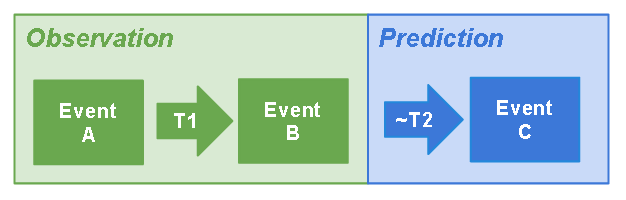
\includegraphics[width=\textwidth]{./img/association_rules.png}
\caption{A general prediction} \label{fig:ass_rule}
\end{figure}


The events forming the \emph{consequent} of our prediction will be alarms raised by the maintenance stations - we want to prevent or be prepared for the alarms happening in the future - and the antecedent can be formed by different kind of elements. Therefore, we will distinguish two main working lines: prediction based on previous alarms (section~\ref{sec:alarm-based-prediction}) and prediction based on external conditions (section~\ref{sec:external}).


\subsection{Prediction based on previous alarms}\label{sec:alarm-based-prediction}
This working line consists of acquiring knowledge on how events are related to each other in terms of occurrence. In other terms, the events in the antecedent of our predictions will be formed by alarms (as well as the consequent, as we said before). Among all the alarms raised on the maintenance stations, some of them may be directly triggered by previous ones, having a direct occurrence relation; or might be caused by the same environmental conditions, being most likely for them to happen along the same time periods. As a result, even in cases where they might seem completely unrelated, the occurrence of one of them can give us information on the chances of others happening within a defined time span.

Our objective is to find and analyse these relations and use them to build useful predictions. Depending on the parameters we use for our knowledge discovery procedures, we might obtain different types of rules. For instance, varying the temporal resolution of our analysis, we might obtain rules to predict events in terms of months, days or hours. Depending on the timespan we work with, our prediction rules may be useful to prevent failures, to be prepared to fix them, or be completely useless if there is not enough anticipation.

It is important to note that in the railway network we are working with, there are different maintenance stations in different railway lines. Neither the maintenance stations or the lines are equal throughout the whole network, and therefore we may have to follow different procedures and expect different results for each of them. Initially, we will treat every station (along with the set of elements under its management) independently, even though we already know their classification and the similarities between them. Unless generalisation is evident and clearly convenient, we will always maintain this separation and obtain a different set of rules for each of them.

Due to the characteristics and large size of the available data, we are likely to find a vast amount of frequent sequences and association rules from which not all of them will be useful for maintenance purposes. Different metrics can be applied to evaluate the \emph{importance} of a rule, such as its confidence (its probability to be true on a given situation), the severity of the predicted events, or its support (absolute frequency of the sequence happening).

A comprehensive analysis is necessary to extract the most useful association rules from the set and discard the others, in order to obtain the most efficient set possible. Additionally, the different metrics can even allow predictions to be filtered in real time, according to the available resources or the desired results.

In figure~\ref{fig:demo_view} we can view an example use case. A maintenance operator could view the alarms which are being raised by the maintenance station (in a similar way as the current systems) and a list of predicted alarms - along with the confidence of the prediction and an estimated time span - based on those past and current alarms.

\begin{figure}[hbtp]
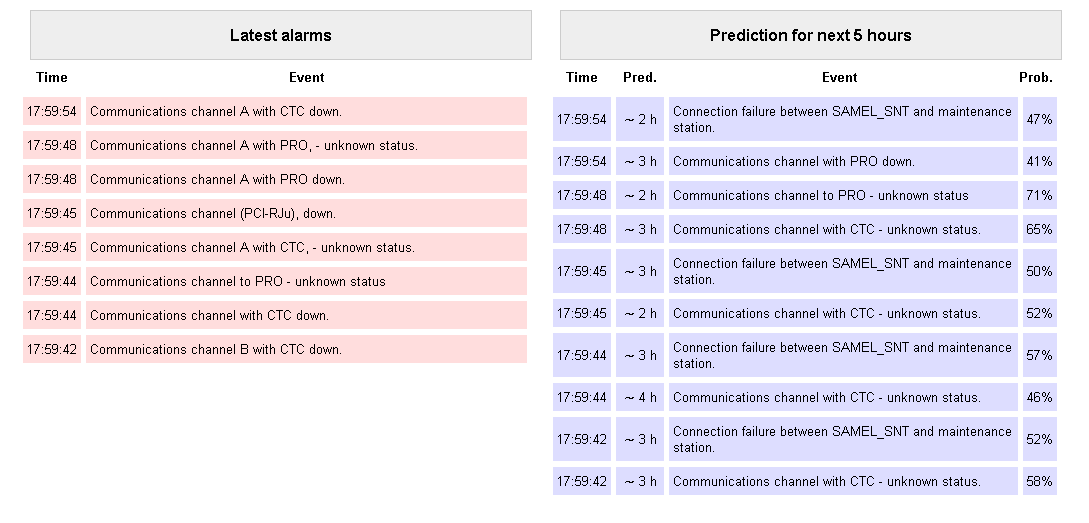
\includegraphics[width=\textwidth]{img/demo_thales.png}
\caption{An example use case} \label{fig:demo_view}
\end{figure}

\subsection{Prediction based on external conditions}\label{sec:external}
This working line consists of acquiring knowledge on the conditions in which alarms are most likely to be raised. The events in the antecedent of our predictions will therefore be variations of different system variables we would have to monitor. This may be the most natural approach for predictive maintenance: trying to observe the environment variations which may be the direct causes of system failures. For example, we might want to analysis which variations of temperature lead to system breakdown, or how slight variations on power supply voltage can indicate a future failure.

However, automatic acquisition of this kind of data is not a trivial issue. With hundreds of elements along the railway lines, and maybe up to dozens of variables to monitor in each of them, it would require an efficient way to obtain this large amount of data.

Currently, the only source of this kind of information we have is the logs maintenance workers fill when performing preventive maintenance procedures. Although we might be able to actually extract useful knowledge from this kind of data, its implementation would not be immediate or easy, as said automatic data acquisition systems would be needed in order for our rules to be applied. For these reasons, we will relegate this kind of predictions to a second place, and focus on alarm-based predictions as mentioned in section~\ref{sec:alarm-based-prediction}.

\section{Knowledge Discovery in Databases}
The whole process we are approaching in this project is usually known as \emph{Data Mining}, or more generally, \emph{Knowledge Discovery in Databases}. A lot of research has been already done on this field which will serve as background for our project, as well as tools and algorithms which have been designed to treat similar problems and which we can adapt or use as base to develop our own\cite{chen1996data, fayyad1996kdd}.

Knowledge Discovery in Databases - or \emph{KDD} - is a term used to describe the procedure of acquiring high-level knowledge from low-level data. As a formal definition, \emph{Knowledge Discovery} is the non-trivial extraction of implicit, previously unknown, and potentially useful information from data~\cite{frawley1992knowledge}. This knowledge is usually found in the form of patterns and relations between variables which were unlikely to be related.

The KDD process involves several steps~\cite{feyyad1996data} which can be summarized as follows:

\begin{enumerate}
 \litem{Understanding the problem:} The first step involves understanding the environment we are studying and gaining relevant prior knowledge. In this step we must identify which goals we want to set for the knowledge discovery process. This is, we must identify the kind of knowledge we want to obtain and the data we can count on for this process.
 \litem{Creating a target dataset:} We will usually need to select a subset of variables from the available datasets. While the system we are studying may need a lot of variables to log events or make data relations, we will not likely need all of them to characterize our problem. Reducing the dimensionality of the problem will provide better results and ease the following steps.
 \litem{Data cleaning and preprocessing:} In this step we have to discern which data is actually relevant and significant for our study, and which is merely noise or outliers which should be disregarded. Operations such as noise modelling or mapping of missing and unknown values are also taken in this step.
 \litem{Data mining:} For this step we must first have decided the purpose of the model derived by the data mining algorithm. For example, summarization, regression, clustering and others. According to our decision, some data mining algorithms will be more appropriate than others.
 \litem{Interpretation of results:} Consists on interpreting the discovered patterns, removing those redundant or irrelevant and translating the useful ones into understandable terms.
 \litem{Consolidation of discovered knowledge:} The discovered knowledge is finally consolidated in an appropriate form. Depending on the context of our project, it might be simply documented or integrated in predictive modules for the analysed systems.
\end{enumerate}

\emph{Data Mining} comprises a large amount of different algorithms which can be used for the Knowledge Discovery process. Depending on the nature of the data on which we will apply these algorithms, and on the kind of knowledge we expect or want to acquire, we will need algorithms of different types.

Different algorithms can usually be classified in the following categories:

\begin{enumerate}
 \litem{Classification:} Learning a function that maps an item into predefined classes.
 \litem{Regression:} Learning a function that maps an item to a predicted variable.
 \litem{Segmentation:} Identifying a set of clusters to categorise the data.
 \litem{Summarization:} Finding a compact description for the data.
 \litem{Association:} Finding significant dependencies between different variables.\cite{Zhao2003association}.
 \litem{Sequence analysis:} Finding frequent sequences or episodes in data~\cite{zhao2003sequential,weiss2002predicting}.
\end{enumerate}

\subsection{Data preprocessing}

Most data mining processes are usually focused on predicting the value of some variables given the value of the rest variables in a given observation. They work with discrete observations for which each of the variables is analysed or predicted. Our case is significantly different, as we have a continuous observation and events which are not modelled as variables. We can easily convert our continuous situation to a discrete one by splitting time into smaller sized periods. Our variables will therefore be the number of times each type of alarm happens during said period, and the time slots will represent the discrete observations. To illustrate this conversion, we have represented an example of the data formats before preprocessing in table~\ref{tab:data_before} and after preprocessing in table~\ref{tab:data_after}.

\begin{table}
\begin{center}
\begin{tabular}{|c|c|c|}
\hline \headcell{Date} & \headcell{Time} & \headcell{Alarm} \\ 
\hline
\hline 01-01-2011 & 00:00 & Alarm A \\ 
\hline 01-01-2011 & 00:30 & Alarm B \\ 
\hline 01-01-2011 & 00:45 & Alarm B \\ 
\hline 01-01-2011 & 01:10 & Alarm C \\ 
\hline 01-01-2011 & 01:20 & Alarm A \\ 
\hline 01-01-2011 & 01:30 & Alarm A \\ 
\hline 01-01-2011 & 01:25 & Alarm C \\ 
\hline 01-01-2011 & 02:20 & Alarm A \\ 
\hline 01-01-2011 & 02:30 & Alarm A \\ 
\hline 01-01-2011 & 02:45 & Alarm B \\ 
\hline ... & ... & ... \\ 
\hline 
\end{tabular} 
\end{center} 
\caption {Continuous observation. Example of data in log format.} \label{tab:data_before} 
\end{table}

\begin{table}
\begin{center}
\begin{tabular}{|c|c|c|c|}
\hline \headcell{Time} & \headcell{Alarm A} & \headcell{Alarm B} & \headcell{Alarm C} \\ 
\hline
\hline 0 & 1 & 2 & 0 \\ 
\hline 1 & 2 & 0 & 2 \\ 
\hline 2 & 2 & 1 & 0 \\ 
\hline ... & ... & ... & ... \\ 
\hline 
\end{tabular} 
\end{center} 
\caption {Example of discretised data} \label{tab:data_after} 
\end{table}

For further simplification, we can even reduce the problem to terms of whether an alarm happens or not, and disregard the number of times each of them happen. This approach would be necessary when treating alarms which are not very frequent, and for which the number of occurrences during an observation will typically vary between 0 and 1. However, for events with a higher occurrence rate, the actual number of occurrences within an observation might be of importance. The optimum approach might vary between situations, and therefore we cannot still decide for one of them at early stages of the project.

It is also important to note that an optimum choice of the sampling time is important. If we want to achieve predictions in time spans of months, it might be inappropriate to choose an observation period of seconds or minutes. For our project, due to the characteristics of the procedures of railway maintenance, we aim to achieve predictions in terms of weeks. Therefore, we have chosen the observation time to be a period of 24 hours. When working with \emph{sequence analysis}, we have also to define additional time constraints\cite{suh2011practical}, such as the maximum distance between the antecedent and consequent, or even between several events on the antecedent (or consequent).

A large amount of existing algorithms have been implemented taking into consideration these issues for sequential analysis~\cite{wu2010sequential}. Some of them will be analysed in order to work as a base or tool for our project.

\section{Working methods} \label{sec:methods}
For the development of this project, we have found a vast amount of useful tools and software which will provide an inestimable help in the different processes of our work. The main tool used will be the \emph{R} language\cite{ihaka1996r}, a very powerful tool commonly used for handling large amounts of data in an efficient way, and for which a vast amount of tools are available for our needs. R, and the IDE we are using, \emph{RStudio}\cite{racine2012rstudio} are open source software and available at no cost.

Due to licensing and compatibility issues, we are not able to use \emph{Microsoft SQL Server} databases to handle data. This is highly inconvenient as the data provided by Thales is in form of MS SQL backup files, which we needed to migrate to a compatible system of our choice: \emph{MySQL}. Given the tabular nature of the data, another solution based on plain text files would not be recommendable - although possible to handle with R - at least at the earliest stages until we analyse all the information and reduce the number of variables to export. In order to perform these migration tasks, a \emph{Windows} platform with \emph{Microsoft SQL Server Express} was required. Migration was successfully possible after slight modification of indexes and field definitions to fix compatibility issues. Once in MySQL format, we can query our data from RStudio without being limited to any kind of platform type or operative system, and will indeed perform further stages of the project under \emph{Unix} platforms.

Among all the available algorithms which can be useful for our project, we have chosen the \emph{cSPADE} algorithm\cite{zaki2001spade} as our starting point. It provides the most straight-away solution for the kind of problem we are approaching, as it considers temporal characteristics and allows us to set time constraints very easily. Other algorithms will be studied and applied at convenience, in order to complement cSPADE and find weak points which we could improve.

Another very useful tools which can be of great help for obtention of this kind of predictions are \emph{Bayesian Networks}\cite{jensen1996introduction}. A Bayesian network is a probabilistic model which represents a set of variables and their conditional dependencies via a directed acyclic graph. A very simplified example can be seen in figure~\ref{fig:bayesian_example} In our case, it would represent the types of alarms and their relation in a graphical network, allowing us to analyse the probabilities of each of them happening within the current observation. Once an alarm has already been raised, its probability can be set to 100\% in the current observation, allowing us to recalculate probabilities for the rest of alarms by application of Bayes theorem. Bayesian networks can be either directly implemented onto any kind of system - as long as we can have real-time information on risen alarms - or be used to extract rules and implement them onto any other kind of system. There are lots of available tools for working with Bayesian networks. Specifically, we will use \emph{GeNIe/SMILE}\cite{druzdzel1999smile} as well as \emph{R libraries} for this purpose.

Table~\ref{tab:objectives_methods} contains a summary of learning objectives and the methods which will be used for each of them.


\begin{figure}[hbtp]

\includegraphics[width=\textwidth]{img/bayesian_example.png}
\caption{An example of a very simple bayesian network} \label{fig:bayesian_example}
\end{figure}

\begin{table}
\begin{tabularx}{\textwidth}{|X|l|X|}
\hline \headcell{Goal} & \headcell{Priority} & \headcell{Method} \\ 
\hline
\hline Perform a preliminary statistical analysis to set the project grounds & Compulsory & Statistical analysis with R \\ 
\hline Identify differences between maintenance stations & Compulsory & Statistical analysis with R \\ 
\hline Obtain rules to predict alarms using data of other alarms occurrence & Compulsory & Data Mining algorithms with R \\ 
\hline Obtain a Bayesian network to overview causal relations between alarms & Compulsory & Bayesian Networks with GeNIe/SMILE \\ 
\hline Validate and evaluate rule sets. Determine confidence of predictions & Compulsory & Cross-validation and confidence analysis with R \\ 
\hline Extract additional rules from Bayesian network for rule-form implementation & Desirable & GeNIE/SMILE \\ 
\hline Identify rule sets which can be applied to different station types & Desirable & Inter-station cross-validation with R \\ 
\hline Obtain rules to predict events using data of system and environment variables & Optional & Data Mining algorithms with R \\ 
\hline Identify which system or environment variables are more decisive for alarm prediction & Optional & Data Mining algorithms with R \\ 
\hline 

\end{tabularx} 
\caption{Summary of project goals and methods} \label{tab:objectives_methods}
\end{table}


\section{Final comments}
The most important thing before starting any other step, is to completely understand the context and scenario of our project. We do not need to fully know and understand the details on the procedures of railway maintenance, as the nature of the machinery performed reparations is not of significant relevance for the achievement of the defined objectives. In any case where we would need better understanding of system functioning - such as for identifying causal relations between failure events - we would need assistance from expert employees directly related with maintenance.

At this point, we have already treated all received data in order to be able to freely handle it without restrictions from any desired system. Required conversions have been performed and all data is already prepared to be loaded and used in R scripts.

We have also defined the learning objectives for the project, and set a ground to achieve them from an \emph{Knowledge Discovery in Databases} approach. Furthermore, we have made a first insight into \emph{Data Mining} techniques and performed a first analysis on their adequacy for our project. Initial tools have already been selected: cSPADE and GeNIe/SMILE.

In the next stage of Trainmining, we will need to make a deeper insight into the provided databases. The procedures which we have already defined (time discretion and definition of observation times) will have to be performed, selecting the exact variables among all of them which are registered for each alarm.

\clearpage


\chapter{Chapter 2}
\section{Database description}\label{sec:database_description}
In order to properly process the data provided in form of database backups, it is of essential importance that we completely understand how data is represented in databases. We will analyse the structure and how data is represented in the provided databases: Antequera, Segovia and Sevilla. Each of these database corresponds to a single \emph{maintenance station}, which comprises a whole railway line with several elements along it. The elements with diagnosis systems which can raise alarms are called \emph{installations}, and have different sets of sensors and other systems to control \emph{field elements}. An schematic representation of this architecture is represented in figure~\ref{fig:arch_stations}. The detailed description of available systems and subsystems is of few interest to us. Initially we will only need to differentiate between maintenance stations and installations.

\begin{figure}[hbt]
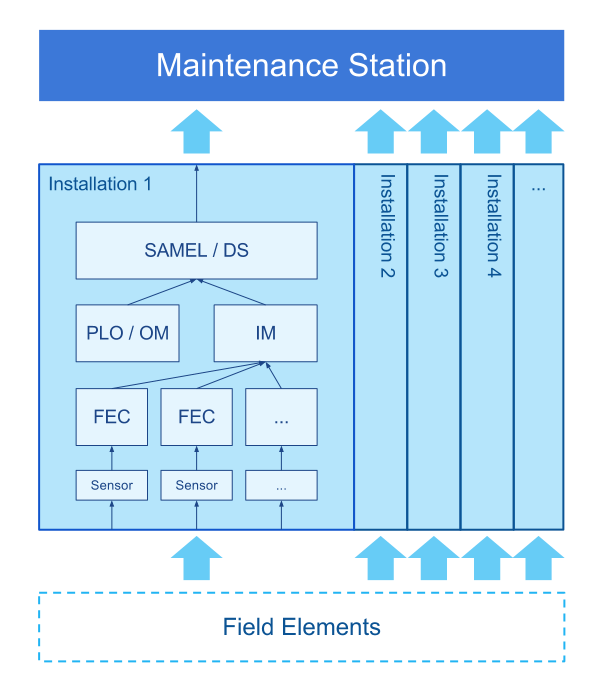
\includegraphics[width=\textwidth]{./img/arch_stations.png}
\caption{Simplified diagram of the maintenance systems architecture} \label{fig:arch_stations}
\end{figure}

Each \emph{maintenance station} has its own unique database, which is of great convenience in order to treat different stations independently. We will start analysing the structure of the main tables of said databases. Due to the high complexity of the maintenance stations, there are a vast amount of tables with configuration parameters and other operational values which are not of interest for our purposes. With assistance from Thales engineers, we have reduced the tables only to those which characterise registered alarms. A total of 4 different tables is used in order to register this information, which are the following:

\begin{description}
\item[Table ER\_ERRORS] This table contains an entry for every alarm received by the maintenance station. Its fields are detailed on table~\ref{tab:table_er_errors}.
\item[Table IG\_INSTALLATIONGENERAL] This table contains information on all the installations managed by the maintenance station. Its fields are detailed on table~\ref{tab:table_ig_installationgeneral}
\item[Table IG\_NODO\_INSTALLATION] This table gathers additional information on installations which are nodes. Nodes are installations which can raise alarms but need a parent installation to send them to the maintenance station. Its fields are detailed on table~\ref{tab:table_ig_nodo_installation}
\item[ERS\_ERRORS\_SAM\_ENCE] This table contains detailed information about the alarms. Its fields are detailed on table~\ref{tab:table_ers_errors_sam_ence}
\item[ERH\_ERRORS\_HSL1] This table is equivalent to ERS\_ERRORS\_SAM\_ENCE. Maintenance stations use one or the other depending on how they receive the alarms. Its only difference with ERS\_ERRORS\_SAM\_ENCE is that registers the method used to receive the alarm. For our purposes it will be treated exactly as its equivalent, and therefore its structure can also be reviewed in table~\ref{tab:table_ers_errors_sam_ence}
\end{description}

Concluding, for each alarm we will have a timestamp and an alarm identifier in table ER\_ERRORS. Alarm identifier is a foreign key which points to table ERS\_ERRORS\_SAM\_ENCE (or equivalent) in which further details of the alarm are saved. Among these details, we can find an installation identifier which specifies which installation has produced the alarm. That identifier is also a foreign key pointing to table DVNI\_INSTALLATIONCODE, in which further details about the installation are stored. Further details on all the database fields are given in tables~\ref{tab:table_er_errors}, \ref{tab:table_ig_installationgeneral}, \ref{tab:table_ig_nodo_installation} and \ref{tab:table_ers_errors_sam_ence}.


\begin{table}
\begin{tabularx}{\textwidth}{|l|X|}
 \hline \headcell{Field name} & \headcell{Description} \\
 \hline
 \hline DVNI\_ERRORNUMBER & Alarm identifier \\
 \hline DVNS\_ERRORTIME & Time-stamp for the alarm \\
 \hline DVNI\_INSTALLATIONCODE & Code of the installation in which the alarm was raised \\
 \hline DVNI\_SENDERINSTALLATIONCODE & Code of the installation from which the alarm was sent (might be different from the one which raised it) \\
 \hline
\end{tabularx}
\caption{Detail of fields on table ER\_ERRORS} \label{tab:table_er_errors}
\end{table}

\begin{table}
\begin{tabularx}{\textwidth}{|l|X|}
 \hline \headcell{Field name} & \headcell{Description} \\
 \hline
 \hline DVNI\_INSTALLATIONCODE & Installation identifier  \\
 \hline DVNI\_SYSTEMCODE & Type of system, as defined in the ``SG\_SYSTEMSGENERAL'' table \\ 
 \hline DVNI\_VERSION & System version \\
 \hline DVAC\_SHORTNAME & Short name of the installation \\
 \hline DVAC\_INSTALLATIONNAME & Name of the installation \\
 \hline DVAC\_LOCATION & Location for the installation \\
 \hline CHK\_IS\_NODE & Whether it is a node (doesn't directly send alarms, only raise them) or not \\
 \hline
\end{tabularx}
\caption{Detail of fields on table IG\_INSTALLATIONGENERAL} \label{tab:table_ig_installationgeneral}
\end{table}

\begin{table}
\begin{tabularx}{\textwidth}{|l|X|}
 \hline \headcell{Field name} & \headcell{Description} \\
 \hline
 \hline IG\_NODO\_INSTALLATION & Identifier of the installation which is a node \\
 \hline DVNI\_FATHER\_INSTALLATION & Identifier of the parent installation \\
 \hline
\end{tabularx}
\caption{Detail of fields on table IG\_NODO\_INSTALLATION} \label{tab:table_ig_nodo_installation}
\end{table}

\begin{table}
\begin{tabularx}{\textwidth}{|l|X|}
 \hline \headcell{Field name} & \headcell{Description} \\
 \hline
 \hline DVNI\_ERRORNUMBER & Alarm identifier \\
 \hline MESSAGE\_ID & Unique alarm identifier \\
 \hline MESSAGE\_TYPE & Type of alarm, always set as ``notification'' (not relevant) \\
 \hline INVOKE\_TYPE & Tells whether the alarm has generated itself due to a connection or disconnection (if type is ``node'') or is generated by a diagnosis system (``saml'') or energy system (``energy'') \\
 \hline INVOKE\_NAME & Irrelevant, always set to ``diagnosis'' \\
 \hline EVENT\_TYPE & Defines the type of alarm which has been generated. Its possible values are listed in table~\ref{tab:field_event_type}. \\
 \hline ADDITIONAL\_TEXT & Alarm code \\
 \hline ADDITIONAL\_INFOS & Additional parameters to be shown in error message \\
 \hline DVNI\_ERRORCATEGORY & Alarm severity. Values from 1 to 5 indicating importance of the alarm, or -1 if the alarm indicates recovery from a previous failure. \\
 \hline
\end{tabularx}
\caption{Detail of fields on table ERS\_ERRORS\_SAM\_ENCE} \label{tab:table_ers_errors_sam_ence}
\end{table}

\begin{table}
\begin{tabularx}{\textwidth}{|l|X|}
  \hline \headcell{Event type} & \headcell{Description} \\
  \hline
  \hline fieldElementAlarm & Alarm related to a field element \\
  \hline fieldElementFailure & Failure in a field element \\
  \hline operatorInformation & Information to the operator \\
  \hline imCpuAndCommunications & Related to IM CPU or IM communications \\
  \hline internalDiagnosis & Internal diagnosis of a system \\
  \hline operationsDiagnosisCommunications & Communication error in Operation and Diagnosis systems \\
  \hline ImFecVersions & IM or FEC version \\
  \hline internalTraces & Internal traces of a system \\
  \hline operatorCommandAnswer & Answer to an operator command \\
  \hline CommProblem & Undefined communication problem \\
  \hline Information & Information message: versions, etc. \\
  \hline CommunicationsAlarm & Procedures and processes to carry information from one point to other \\
  \hline QualityOfServiceAlarm & Loss of quality of service \\
  \hline ProcessingErrorAlarm & SW or processing error \\
  \hline EquipmentAlarm & Equipment failure \\
  \hline EnvironmentAlarm & Related to the environment where the system is located \\
  \hline other & Other \\
  \hline
\end{tabularx}
\caption{Description of values for the field EVENT\_TYPE} \label{tab:field_event_type}
\end{table}
\clearpage
\section{Reduced representation of alarms}\label{sec:reduced_alarms}
In section~\ref{sec:database_description} we have seen a deep definition of all the tables characterising registered alarms. Each of these tables contain several fields, which in total makes an inconvenient large number of variables. While all of them are necessary for correct system function and maintenance purposes, not all of them will be necessary for us to work with alarms.

In order to characterise an event, the main things we need to know can be reduced to three variables:
\begin{itemize}
\item What has happened
\item When has it happened
\item Where has it happened
\end{itemize}

In section~\ref{sec:database_description} we have seen other variables which can provide additional information which - although not essential - can be useful. Specifically, we think the following data can be of possible interest:

\begin{itemize}
\item How severe the event is (severity)
\item Which type of event has happened (event type)
\end{itemize}

These variables can help us to classify alarms or give more importance to those which are more severe. As this information is already provided on given databases, we will keep it and use it for better alarm classification and filtering. However, none of them are essential in order to characterise alarms, as both of them give information which is already implicit in our previous \emph{``what has happened''} variable. Specifically, this information will be of great help in order to make a preliminary statistical insight on the events of the databases, for which a generalisation in terms of severity and category can help us have a better overview of the situation.

We have to identify which fields on our database corresponds to each of the variables we want to obtain. A direct relation is not possible, as details on \emph{what} has happened is registered in several fields of the database. This is necessary for maintenance purposes and better alarm handling in the maintenance station, but for our purposes we should identify \emph{what} has happened with a single variable.

In our database, we have unique alarm identifiers for each of the alarms. For better handling and understanding of what is happening, we will use the textual identifier of the events to identify them. This identifier is gathered on the \emph{ADDITIONAL\_TEXT} field, and can be translated to a full comprehensive human-readable message by the maintenance station. Furthermore, there is additional data to fill in details about the message. For example, we can have an alarm such as ``Communication channel with \emph{X} down'', being \emph{X} an additional parameter saved in the \emph{ADDITIONAL\_INFOS} field. Here we can follow two different approaches: disregard the information about \emph{X}, and just treat it as a ``Channel down'' error; or easily build a compact representation including both variables, such as ``channel.down/x''.

\section{Statistic analysis}
In order to obtain a first general insight of what has happened during the time comprised by our backup data, we will perform a high-level preliminary statistic analysis. In order to achieve a qualitative idea of the type of events, we will use the additional variables we mentioned in section~\ref{sec:reduced_alarms}: severity and event type. These variables provide an already given alarm classification of interest for maintenance operators.

For this purpose, the R language provides a large amount of useful tools which can handle large amounts of data in a very efficient way\cite{quick2010statistical}.

\subsection{Event type distribution}
The first analysis we will perform consists on checking which event types appear in each maintenance station, and which percentage of the total amount of alarms corresponds to each of them. This will help us understand the nature of the events which are usually happening on our railway line.

First of all we will obtain a list of all the types found in each of the stations. We already described in table~\ref{tab:field_event_type} all the possible values for this field, but depending on the diagnosis systems installed on each of the stations, a different subset of them will be used. The list of events for each of the stations is given in tables \ref{tab:field_event_type_antequera} (Antequera), \ref{tab:field_event_type_sevilla} (Sevilla) and \ref{tab:field_event_type_segovia} (Segovia).

\begin{table}
\begin{tabularx}{\textwidth}{|l|X|}
  \hline \headcell{Event type} & \headcell{Description} \\
  \hline
  \hline fieldElementAlarm & Alarm related to a field element \\
  \hline fieldElementFailure & Failure in a field element \\
  \hline operatorInformation & Information to the operator \\
  \hline imCpuAndCommunications & Related to IM CPU or IM communications \\
  \hline internalDiagnosis & Internal diagnosis of a system \\
  \hline operationsDiagnosisCommunications & Communication error in Operation and Diagnosis systems \\
  \hline CommunicationsAlarm & Procedures and processes to carry information from one point to other \\
  \hline
\end{tabularx}
\caption{Event types found in Antequera} \label{tab:field_event_type_antequera}
\end{table}

\begin{table}
\begin{tabularx}{\textwidth}{|l|X|}
  \hline \headcell{Event type} & \headcell{Description} \\
  \hline
  \hline fieldElementAlarm & Alarm related to a field element \\
  \hline fieldElementFailure & Failure in a field element \\
  \hline operatorInformation & Information to the operator \\
  \hline imCpuAndCommunications & Related to IM CPU or IM communications \\
  \hline internalDiagnosis & Internal diagnosis of a system \\
  \hline operationsDiagnosisCommunications & Communication error in Operation and Diagnosis systems \\
  \hline CommunicationsAlarm & Procedures and processes to carry information from one point to other \\
  \hline Other & other \\
  \hline
\end{tabularx}
\caption{Event types found in Sevilla} \label{tab:field_event_type_sevilla}
\end{table}


\begin{table}
\begin{tabularx}{\textwidth}{|l|X|}
  \hline \headcell{Event type} & \headcell{Description} \\
  \hline
  \hline CommProblem & Undefined communication problem \\
  \hline Information & Information message: versions, etc. \\
  \hline CommunicationsAlarm & Procedures and processes to carry information from one point to other \\
  \hline ProcessingErrorAlarm & SW or processing error \\
  \hline EquipmentAlarm & Equipment failure \\
  \hline EnvironmentAlarm & Related to the environment where the system is located \\
  \hline
\end{tabularx}
\caption{Event types found in Segovia} \label{tab:field_event_type_segovia}
\end{table}

From these tables we can observe that alarm types in Antequera and Sevilla are the same (except for unclassified alarms in Sevilla marked as ``other''). From this we can infer that diagnosis systems in these two stations are the same or very similar, as confirmed by Thales' engineers. Segovia however presents a different - although also expectedly similar - set of alarm categories. This is an indicator of diagnosis systems being very different in Segovia than in the other two stations, as confirmed by Thales' engineers.

For better overview of distribution of these alarm types, we will create charts of their respective percentages for each of the stations. These charts can be seen in figures \ref{fig:antequera_chart} (Antequera), \ref{fig:segovia_chart} (Segovia) and \ref{fig:sevilla_chart} (Sevilla).

\begin{figure}[htb]
 \centering
 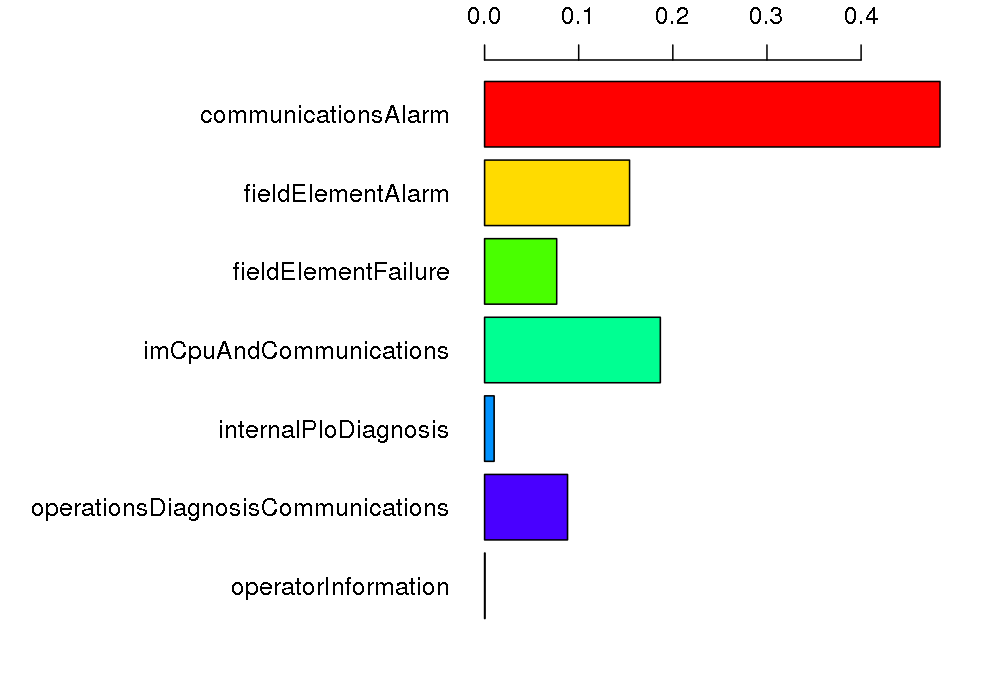
\includegraphics[width=\textwidth]{./img/antequera_graph.png}
 \caption{Alarm information for Antequera}
 \label{fig:antequera_chart}
\end{figure}
\begin{figure}[htb]
 \centering
 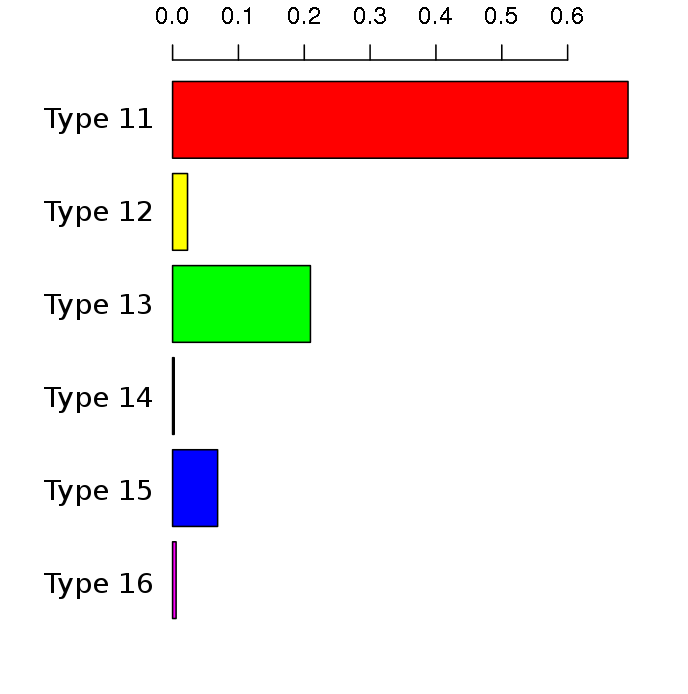
\includegraphics[width=\textwidth]{./img/segovia_graph.png}
 \caption{Alarm information for Segovia}
 \label{fig:segovia_chart}
\end{figure}
\begin{figure}[htb]
 \centering
 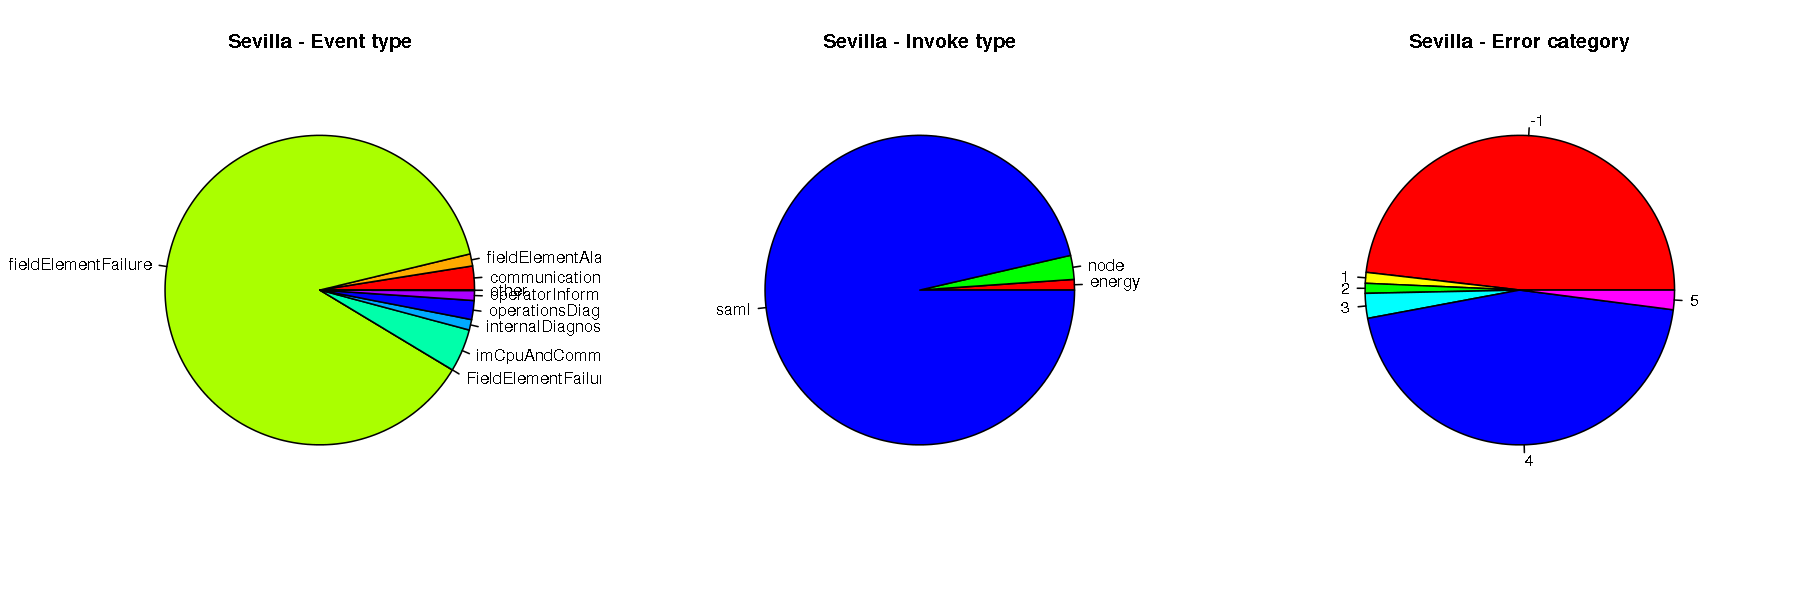
\includegraphics[width=\textwidth]{./img/sevilla_graph.png}
 \caption{Alarm information for Sevilla}
 \label{fig:sevilla_chart}
\end{figure}

\clearpage

We can see that in all of the stations, a single alarm type predominates among all of them. Specifically, we have a vast majority of communication alarms in Antequera and Segovia, and a majority of field element failure alarms in Sevilla. This is not surprising due to the considerable differences between all of them, but can become a problem as the other categories may be too small compared to these main ones when performing Data Mining techniques, obtaining less information - or none at all - from them.

In this direction, it is possible that further actions are required in order to compensate these differences, and avoid that more frequent alarms overshadow the less frequent ones.

\subsection{Daily correlation}
In order to find further differences or similarities between the different stations, we will observe how alarm types are correlated to each others\cite{edwards1976introduction}. That is, how frequent is to find alarms of two specific types happening together during the same short period. For a first insight, we will analyse correlation during daily observations. This correlation information will not be of immediate help in order to predict alarms, as predicting the most frequent alarm type given some conditions is of very little - if any - help. However, it will give us a first idea on how strongly alarms are related to each others.

The result of this correlation is represented in figures \ref{fig:anteq_corr} (Antequera), \ref{fig:segovia_corr} (Segovia) and \ref{fig:sevilla_corr} (Sevilla).

\begin{figure}[htb]
 \centering
 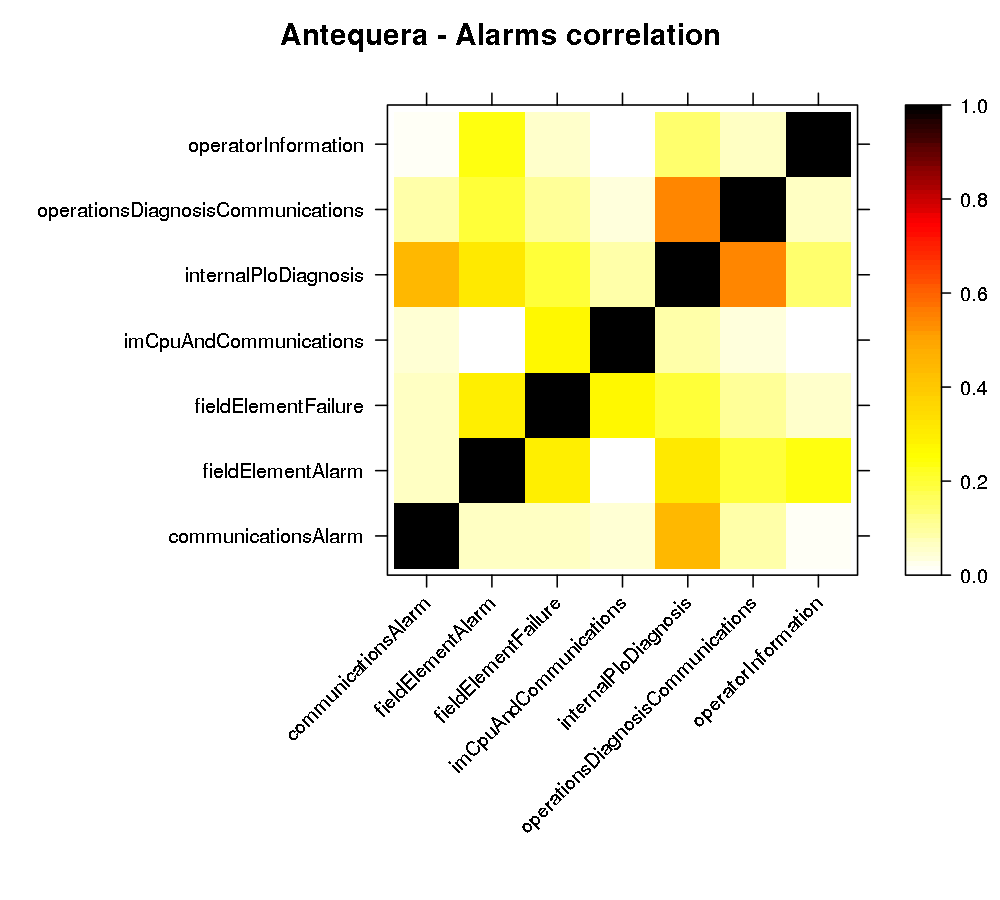
\includegraphics[width=\textwidth]{./img/antequera_corr.png}
 \caption{Daily correlation for Antequera} \label{fig:anteq_corr}
\end{figure}
\begin{figure}[htb]
 \centering
 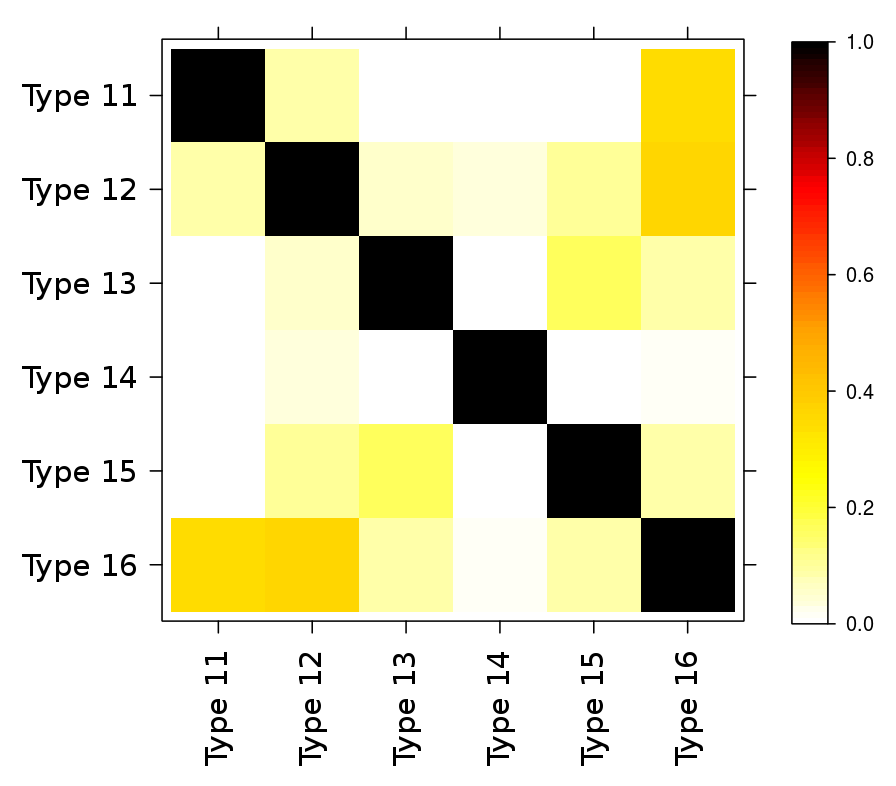
\includegraphics[width=\textwidth]{./img/segovia_corr.png}
 \caption{Daily correlation for Segovia} \label{fig:segovia_corr}
\end{figure}
\begin{figure}[htb]
 \centering
 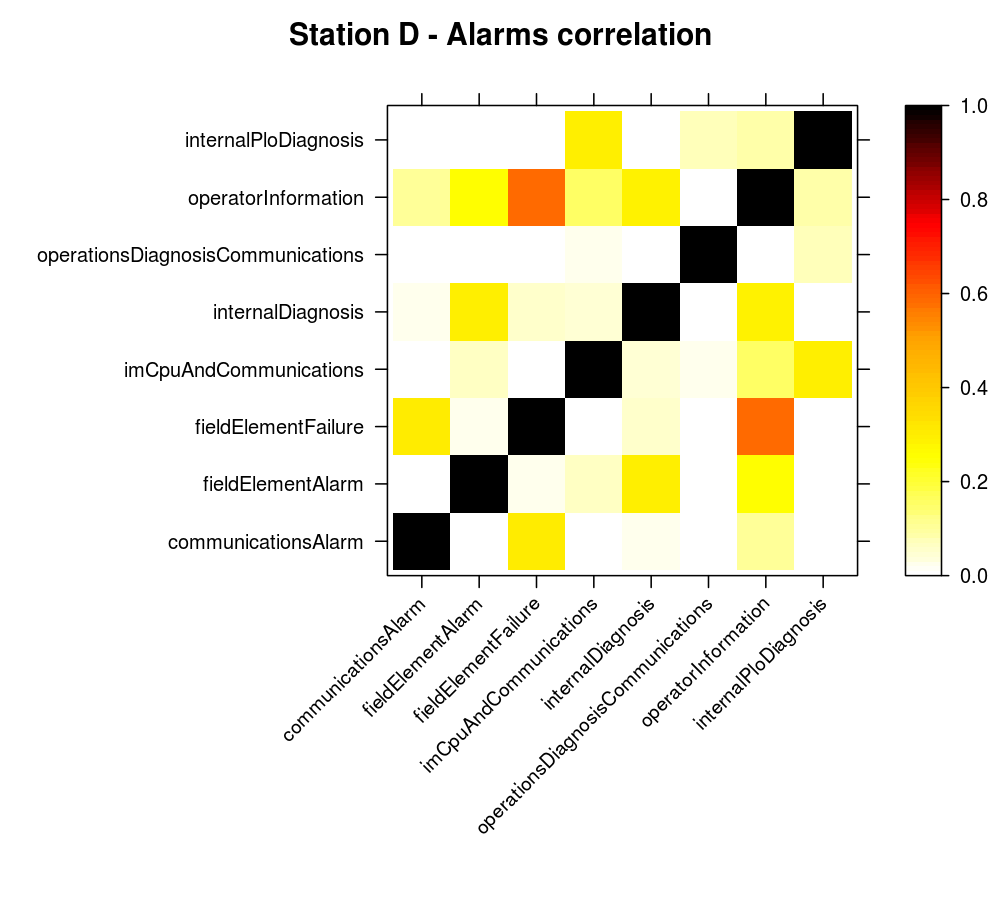
\includegraphics[width=\textwidth]{./img/sevilla_corr.png}
 \caption{Daily correlation for Sevilla} \label{fig:sevilla_corr}
\end{figure}

\clearpage

At first sight, we can affirm that these relations are different even in Sevilla and Antequera, which we found to have similar diagnosis systems. This indicates that, even with similar diagnosis systems, the systems conforming both lines are different. This is indeed confirmed by Thales' engineers, as Antequera station controls a high speed line, while Sevilla corresponds to a commuter line.

Furthermore, we can see strong correlations in Sevilla (Field element failure and operator information) and Segovia (Communications alarms and processing error alarms). As we don't have deep information of the nature of these categories, we can't affirm that this high correlation is due to any causal relation. However, we observe that both these cases show high correlation for the type of alarm which is more frequent in each station, so uneven distribution of alarms might be the cause of this apparent relation between alarms.

From this analysis we can conclude the significant differences in alarm relations between stations, confirming our first thoughts of impossibility of reducing the problem by generalising and merging data from different stations. Further analysis using specific alarm identifiers instead of categories will be needed to obtain relevant results.

\subsection{Hourly timeline}
As an additional first analysis, we wanted to overview the variation of alarm occurrence during the day. During a day, high differences in environment can be experimented which can affect systems in different ways. For instance, temperatures or train affluence can be very different from 4:00 AM to 1:00 PM. These differences can also be found during higher periods, for instance between weekdays and weekends, or between summer time and winter. To start with a specific observation period, we will perform a first analysis between day hours, leaving the other cases for future stages if considered adequate.

Charts with this analysis can be seen in figures \ref{fig:antequera_timeline} (Antequera), \ref{fig:segovia_timeline} (Segovia) and \ref{fig:sevilla_timeline} (Sevilla).

\begin{figure}[htb]
 \centering
 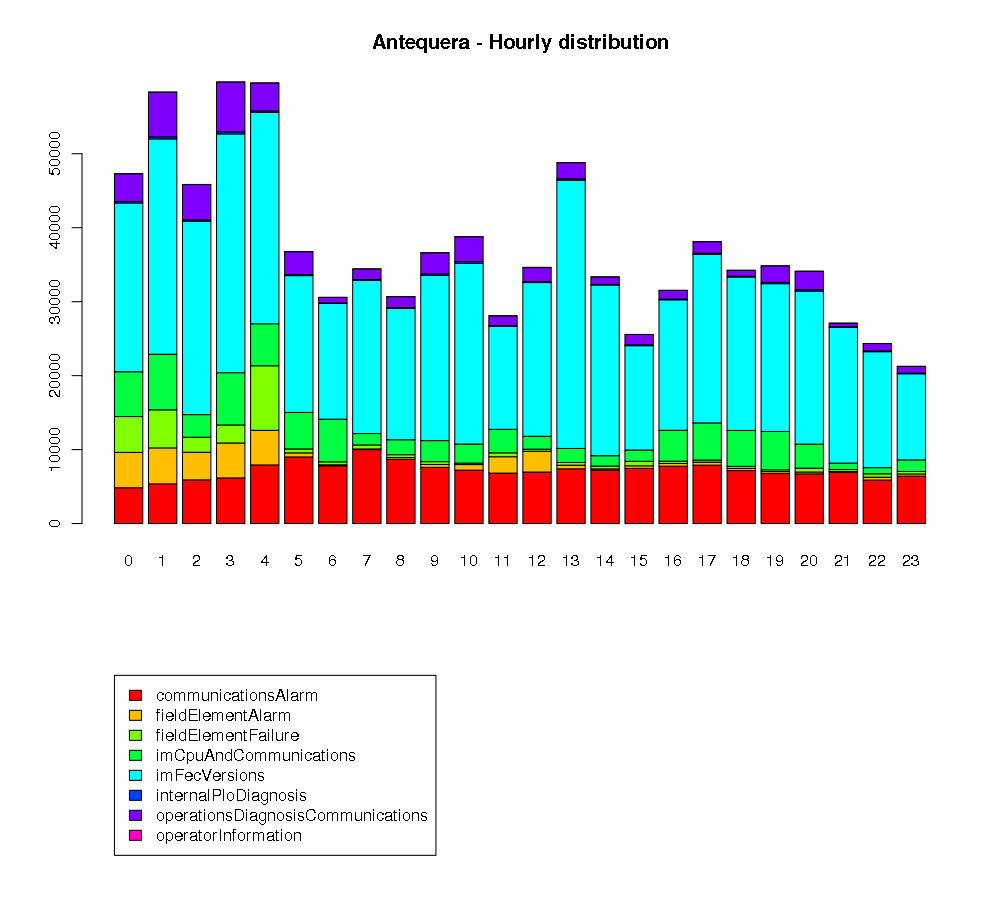
\includegraphics[width=\textwidth]{./img/antequera_timeline.png}
 \caption{Hourly distribution for Antequera (stacked)} \label{fig:antequera_timeline}
\end{figure}
\begin{figure}[htb]
 \centering
 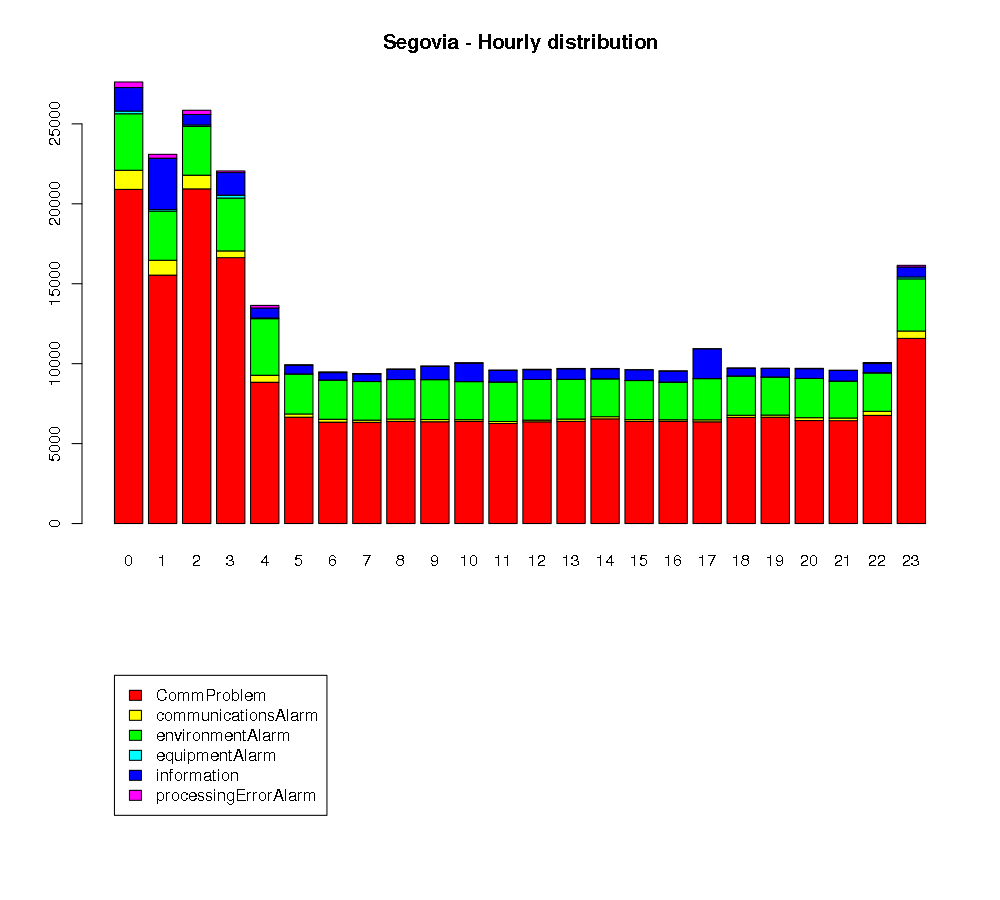
\includegraphics[width=\textwidth]{./img/segovia_timeline.png}
 \caption{Hourly distribution for Segovia (stacked)} \label{fig:segovia_timeline}
\end{figure}
\begin{figure}[htb]
 \centering
 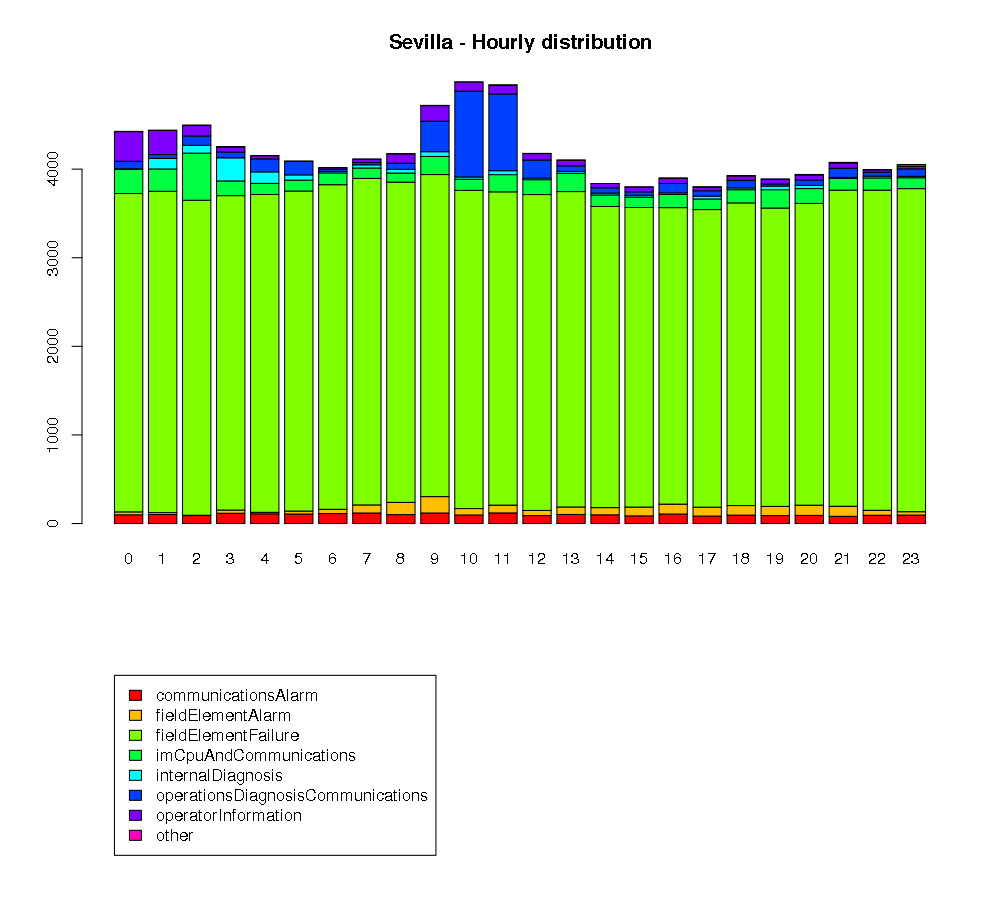
\includegraphics[width=\textwidth]{./img/sevilla_timeline.png}
 \caption{Hourly distribution for Sevilla (stacked)} \label{fig:sevilla_timeline}
\end{figure}

\clearpage

\section{Data preprocessing}\label{sec:data_preprocessing}
As we already mentioned, most data mining processes are usually focused on predicting the value of some variables given the value of the rest variables in a given observation. They work with discrete observations for which each of the variables is analysed or predicted. In our databases we have continuous observations, which need to be transformed into discrete observations\cite{zaki2001spade}.

Depending on the specific application we are using, we can need to transform this data into two possible formats. The first one is the called \emph{basket format}. The most typical example usually used to explain it is a registry of clients of a shop which keeps lists of what the clients buy (hence the name). Therefore, for each observation (often called \emph{transactions} again as an analogy to clients buying in a shop) we will have a list of items happening during that observation (or bought in that transaction). It is important to note that we will keep the same number of variables as in our original data, only that we will stack several items in single entries to obtain discrete observations. It is also important to be careful with which variables we are stacking. While we need to combine all the alarms happening during the same period, it is important not to lose or combine the Installation value. As a result, time identifiers won't be unique in the whole transformed database, but the pair time identifier-installation identifier will.

An example can be seen in tables \ref{tab:data_before_discret} and \ref{tab:basket_example}. Table~\ref{tab:data_before_discret} is an example of the original data, and table~\ref{tab:basket_example} is the equivalent data transformed into basket format.

The second possible transformation is to represent the occurrence of each alarm with an additional variable. This means that we will need as many variables as the total number of possible different alarms in our system. Same as before, we must be careful to preserve data on installations, and create independent observations for each time slot and each installation. Each additional variable can represent the alarms in different ways. Either in a boolean sense (whether the alarms happens at least once or not at all) or the specific number of times the alarm has happened. In order not to lose information at this stage of processing, we will keep the specific amount of times each alarm has happened, which can be easily reduced to a boolean variable if appropriate for the application.

This second case is indeed a more strict representation of the \emph{basket format}. While in basket format we just needed a single variable where we could add all the alarms in the form of a list, here we need to specify exactly the number of times all the variables have happened. Both of them are equivalent and we can easily convert data from one format to another, but as different algorithms will work specifically with one of each forms of representation, it's convenient to perform both transformations from original data and use each one accordingly.

An example of this transformation can be seen in tables \ref{tab:data_before_discret} and \ref{tab:expanded_example}. Table~\ref{tab:data_before_discret} is an example of the original data, and table~\ref{tab:expanded_example} is the equivalent data discretised with additional variables.

These transformations have been automatised with R scripts, in a way so we can easily repeat these processes for different time spans. This will allow us to work at any moment with different time resolutions without any significant additional work for further transformations.

\begin{table}
\begin{center}
\begin{tabular}{|c|c|c|}
\hline \headcell{Timestamp} & \headcell{Installation} & \headcell{Alarm} \\ 
\hline
\hline 01-01-2011 00:00 & 0 & Alarm A \\ 
\hline 01-01-2011 00:30 & 0 & Alarm B \\ 
\hline 01-01-2011 00:45 & 1 & Alarm B \\ 
\hline 01-01-2011 01:10 & 0 & Alarm C \\ 
\hline 01-01-2011 01:20 & 0 & Alarm A \\ 
\hline 01-01-2011 01:22 & 0 & Alarm A \\
\hline 01-01-2011 01:25 & 1 & Alarm C \\ 
\hline 01-01-2011 01:30 & 1 & Alarm A \\ 
\hline 01-01-2011 02:20 & 0 & Alarm A \\ 
\hline 01-01-2011 02:30 & 1 & Alarm A \\ 
\hline 01-01-2011 02:45 & 0 & Alarm B \\ 
\hline ... & ... & ... \\ 
\hline 
\end{tabular} 
\end{center} 
\caption {Continuous observation. Example of alarms in log format.} \label{tab:data_before_discret} 
\end{table}

\begin{table}
\begin{center}
\begin{tabular}{|c|c|c|}
\hline \headcell{Time} & \headcell{Installation} & \headcell{Alarms} \\ 
\hline
\hline 0 & 0 & A, B \\ 
\hline 0 & 1 & B \\ 
\hline 1 & 0 & C, A, A \\ 
\hline 1 & 1 & C, A \\ 
\hline 2 & 0 & A, B \\ 
\hline 2 & 1 & A \\ 
\hline ... & ... & ... \\ 
\hline 
\end{tabular} 
\end{center}
\caption{An example of discretised data in basket format.} \label{tab:basket_example}
\end{table}

\begin{table}
\begin{center}
\begin{tabular}{|c|c|c|c|c|}
\hline \headcell{Time} & \headcell{Installation} & \headcell{Alarm A} & \headcell{Alarm B} & \headcell{Alarm C} \\ 
\hline 
\hline 0 & 0 & 1 & 1 & 0 \\ 
\hline 0 & 1 & 0 & 1 & 0 \\ 
\hline 1 & 0 & 2 & 0 & 1 \\ 
\hline 1 & 1 & 1 & 0 & 1 \\ 
\hline 2 & 0 & 1 & 1 & 0 \\ 
\hline 2 & 1 & 1 & 0 & 0 \\ 
\hline ... & ... & ... & ... & ... \\ 
\hline 
\end{tabular} 
\end{center} 
\caption {Example of discretised data} \label{tab:expanded_example} 
\end{table}

\clearpage

\section{Final comments}
After this step, we have a complete understanding of the database models and how alarms are represented in the provided logs. The preliminary statistic analysis has also provided additional information on the data which will help us to fine-tune actions taken in future steps. 

Furthermore, we are already prepared to load our data into our selected software solutions and start with the \emph{Data Mining} processes. In next steps, we will directly use data in the format here presented as input for already existing data mining solutions, which we will use as starting point for our knowledge discovery process. It is possible that additional transformations are found to be required in further steps of the project, case in which we would have to return to this point and perform whichever process is required by any other algorithm or software.

Specifically, we will continue our work with two solutions: the \emph{cSPADE} algorithm and the \emph{GeNIe/Smile} framework. cSPADE is an implementation of a data mining algorithm which looks for frequent sequences in our database. It needs data in the aforementioned \emph{basket format} - as shown in table~\ref{tab:basket_example} - and will help us obtain association rules to obtain predictions. At the same time, we will work on a relational model using \emph{bayesian networks}, for which we will use the \emph{GeNIe/SMILE} framework. This framework needs the data input to be in the extended format we mentioned in section~\ref{sec:data_preprocessing} and exemplified in table~\ref{tab:expanded_example}.

We have selected an observation time of 24 hours, which will affect the time over which we can make sensible predictions. It is possible that we need to change it to analyse different possibilities, which can be easily done with the R scripts developed in this stage. This will allow comparison of results using different observation spans.

\clearpage


\chapter{Chapter 3}
\section{Introduction}
\label{sec:datamining}
In previous stages of our project we have performed preliminary analysis on our data (mostly statistical) as well as the necessary preprocessing to apply different learning techniques in the following stages. Once we have completed these tasks, it is now time to perform the techniques from which the actual knowledge will be obtained.

This step, usually refered to as \emph{Data Mining} is the most important in the whole \emph{knowledge discovery} procedure. Although data analysis and preprocessing do have a big impact on the quality of the results we will be able to achieve in the end, the choice of an appropriate data mining algorithm is essential for the whole procedure to work.

In order to find the most adequate techniques for knowledge discovery in our project, we will start making a general survey on all the available techniques. Due to the vast amount of already existing implementations available for each of the different data mining categories, we won't have to make an implementation from scratch but adapt one of the already existing implementations to the characteristics of our problem by setting the necessary constraints.

To begin with, we will describe the categories in which all the different algorithms are usually classified. This classification is usually made as follows:

\begin{enumerate}
 \litem{Classification:} Consists on finding functions to map items into already existing classes according to their parameters or characteristics.
 \litem{Regression:} Algorithms aimend to learn functions to predict the value of some variables from other variables or previous values of the same one.
 \litem{Segmentation:} Consists on finding a set of clusters or segments in which the existing items can be categorised.
 \litem{Summarization:} Algorithms used to find compact description for existing data items.
 \litem{Association:} Learning significant relations or dependencies between different variables.\cite{Zhao2003association}.
 \litem{Sequence analysis:} Finding frequent sequences or episodes in data~\cite{zhao2003sequential,weiss2002predicting}.
\end{enumerate}

\emph{Segmentation} and \emph{summarization} algorithms seem to be obviously out of the question, as their functionality differs completely from the objectives we want to achieve in our project. \emph{Regression} algorithms are inadequate as well due to the nature of our data. We do not count on variables whose future value we want to predict.

\emph{Classification} algorithms might not seem like a good choice at first, as we do not have the need to classificate the events into any existing categories. However, if we define an appropriate set of categories and an appropriate model of items to classify, classification algorithms can be actually useful for our tasks. If we model the current events as the \emph{item} to classify, and the possible categories as the possible events which can happen in the future, we can actually classify the current situation (defined by the events which have already happened) into possible categories each defining what would happen next.

However, \emph{sequence analysis} seems to be the most appropriate category at at first glance: we count on historic data from the past and we want to find event patterns from which we can foresee future events. Patterns which are frequent offer useful information in this direction. If we know a set of several events which often happen in the same sequence, we can expect the later events in the sequence to happen once we have already seen the first ones.

These sequences offer a good starting point, but it is important to realize that \emph{frequency} in a pattern refers to the total of events happening during the observated period, and does not indicate in any way the \emph{probability} of the last events in a sequence to happen once the first ones have been acknowledged. In other words, we want to obtain predictions with a high \emph{probability} rather than a high \emph{frequency}.

In this direction, we will use the approach of the \emph{association} algorithms. Using frequent sequences as an starting point, we will build \emph{association rules} which will relate events in the form of boolean variables.

Therefore, this is the most appropriate approach, as it addresses our problem directly without the need of transforming it into a different kind of situation.

\section{Acquisition of association rules}
\label{sec:rule_model}
As we mentioned previously, the most appropriate way to address our problem is the construction of a model based on association rules. This approach consists on building association predictive rules using frequent secuences in our available data as a base.

First of all we must therefore obtain all potential sequential information (patterns) from our database, as mentioned. These sequences will be of the form $\{A, B\} \longrightarrow \{C, D\} \longrightarrow \{E, F\}$ and will serve as a basis to build candidate \emph{association rules}. This step is explained with further details on section~\ref{sec:mining_sequences}.

Using the frequent sequences obtained from the first step, we can build \emph{candidate association rules}. Candidate association rules are of the form $\{A, B\} \xrightarrow{T} \{C\}$. It is important to notice that in these rules we are putting additional temporal information (a distance of T between terms). This temporal information is not implicit in our previous temporal sequences, but can be inferred from the conditions used on the process to obtain them. This will be explained in detail in section~\ref{sec:assoc_rules}.

Finally, we must check which of these \emph{candidate association rules} are actually good predictive rules, and obtain a precise measure of \emph{how good} they are. Specifically, we will measure the \emph{certainty} (precision) of the predictions made by using these rules and the \emph{amount of events} (recall) they are able to predict. This step will be explained in detail in section~\ref{sec:validation_evaluation}.

The whole procedure can be summarized in the following steps:
\begin{enumerate}
\item Mining frequent sequences
\item Building candidate association rules
\item Validate the obtained rules
\end{enumerate}

These steps will be further described in the following sections.

\subsection{Obtaining frequent sequences}
\label{sec:mining_sequences}
The first step for our chosen approach is to find frequent sequences in our datasets. Frequent sequences will be good candidates from which we can be able to obtain association rules -- if there is an unknown causal relation between two events, they will appear together considerably often. Several algorithms have been developed in the past in order to approach this task of finding frequent sequences. Some examples are the \emph{GSB}\cite{zaki2001spade} algorithm and the \emph{SPADE}\cite{zaki2001spade} algorithm, being the later an alternative to the first with better performance and results.

The procedure of finding frequent sequences in a dataset mainly consists on an iterative analysis of all the possible combinations of elements of the database in sequences. For example, the GSB algorithm can be roughly described as follows:

\begin{enumerate}
\item All the possible items (events) of the database are counted. These elements can be seen as sequences of length 1, which will be subsequences of any other larger sequence.
\item All the possible length 2 candidates are generated, as combination of length 1 sequences
\item The database is scanned to calculate the support of generated length 2 candidates
\item Length 3 candidates are generated as addition of length 1 sequences to length 2 sequences whose support is higher than a given minimum
\item The process is repeated till no candidates have high enough support
\end{enumerate}

In other words, the candidates are created in a tree fashion, by adding length 1 sequences (possible terms) to elements in a level. If a branch reaches the minimum required support value, it stops growing, as adding more terms to the sequence will make it more specific and necessarily less frequent.

The support of a sequence is calculated as the number of times it happens in our dataset. The support is usually expressed as a percentage of the whole amount of sequences in the database, but it is important to note that this parameter is not related in any way with the confidence or precision of any prediction we might do with the given pattern. A deeper approach on this issue will be described later in this document.

More information on GSB and SPADE algorithms can be found in \cite{zaki2001spade, zhao2003sequential, srikant1996mining}. Although It is not our priority now to study these algorithms in depth, previous work shows a better performance for SPADE than for GSB, and therefore it will be our algorithm of choice for our work. Furthermore, SPADE implementations are conveniently available in R\cite{ihaka1996r} libraries, which will allow us to easily execute the algorithm on our datasets.

\subsubsection{Defining constraints}
One of the main problems we find when we look for frequent sequences in our database, is that not any sequence -- although frequent -- is useful for our purposes. In the end our goal is to make predictions, for which obtaining these frequent patterns is useful. However, our project context -- and sometimes common sense -- may put additional conditions on \emph{which} kind of predictions are useful; and therefore, \emph{which} kind of patterns we must look for.

For instance, due to the characteristics of our systems, it might not be possible to perform maintenance tasks in short periods of time. Sequences showing us that \emph{A} always breaks within one hour after \emph{B} breaking might not be useful even if we can obtain a very high certainty of that prediction. If we need to buy new pieces to fix B, and those pieces are usually delivered in terms of weeks, knowing that \emph{B} will break one hour before it breaks would not give us any advantage over waiting for it to break and notice without any prediction.

In other words: we need to define temporal constraints in order to obtain sensible predictions\cite{zaki2000cspade}. These constraints are the following:

\begin{description}
\item[Observation time.] We must define for how long we want to take events into account. For example, our predictions for tomorrow will be most likely be made taking into account today's events, as those from last week are less likely to be related with those happening in the short future.
\item[Minimum gap.] This is the minimum amount of time in which we want to predict events. For instance, a gap of 0 would result in predictions for events simultaneous to the observed ones, while a gap of 1 would result in predictions only for the following observation periods.
\item[Maximum gap.] The maximum amount of observations between events in our sequences. By fixing it to the same amount as minimum gap we can obtain sequences with a fixed gap between events.
\item[Maximum window.] This is the maximum temporal length for our sequences. It is important to stress that this is the length of the whole sequence, while the gap is the separation of events within a sequence.
\end{description}

Given these constraints, we have sequences with the following structure:

$$\{A, B\} \xrightarrow{T_1} \{C, D\} \xrightarrow{T_2} \{E, F\}$$

Where $mingap \leq \{T_1, T_2\} \leq maxgap$, and $T_1+T_2 \leq maxwin$. It is important to remark that these temporal conditions are not inherent to the sequences obtained by the SPADE algorithm. As we mentioned in section \ref{sec:mining_sequences}, sequences are built from all the possible combination of events, and then their support is calculated by checking how many times that sequence appears in the database. It is in support calculation where these constraints apply, but the candidate sequences do not contain any temporal information at all. We will only know that their values will be comprised within the ranges we have defined.

In this sequence we have three terms with two events each. In order to build association rules, it is very convenient to limit the number of terms to two -- a single \emph{antecedent} and a single \emph{consequent}. Furthermore, it is very convenient to limit the number of events to one, in order to make individual predictions for each of the events (which may have, for example, different certainties). 

Therefore, the previous example sequence can be divided in three subsequences of two terms:
$$\{A, B\} \longrightarrow \{C, D\}$$
$$\{C, D\} \longrightarrow \{E, F\}$$
$$\{A, B\} \longrightarrow \{E, F\}$$

And, furthermore, each of them can be divided into two subsequences with only one item in the last term:

$$\{A, B\} \longrightarrow \{C\}$$
$$\{A, B\} \longrightarrow \{D\}$$
$$\{C, D\} \longrightarrow \{E\}$$
$$\{C, D\} \longrightarrow \{F\}$$
$$\{A, B\} \longrightarrow \{E\}$$
$$\{A, B\} \longrightarrow \{F\}$$

These sequences are in fact subsequences of the original one, and therefore their individual support values will always be higher than the support original one. This means that these subsequences will already have been obtained as frequent sequences by the SPADE algorithm, without the need of performing division on the longer sequences. As a result, we can simply drop the sequences whose length or complexity is inconvenient for our purposes, as their shorter subsequences will be already found by SPADE.

This results in additional length constraints:
\begin{description}
\item[Maximum terms.] The maximum number of terms in the sequence. In our previous example, we should have set it to \emph{2}.
\item[Maximum items per term.] This condition defines the maximum amount of items in each of the terms of the sequence. This is \emph{not exactly} what we wanted to achieve with our second division of sequences, as we only want to apply this condition to the last term and not to all of them. In our previous example, we would have to set this limit to 1 but only for the last term of the sequence.
\end{description}

Both these groups of constraints must be applied within the process of the algorithms which will obtain the frequent sequences from our database. The length constraints will limit the construction of \emph{candidate sequences} and the temporal constraints will put conditions to the calculation of \emph{sequence support}. Its implementation must therefore be made into the sequence mining algorithms.

An extended version of the SPADE algorithm has been developed to include some of these constraints which were not contemplated by the original SPADE implementation. The \emph{cSPADE} algorithm\cite{zaki2000cspade,wu2010sequential} provides an implementation taking into account all these mentioned conditions. It is available as an R implementation under the library \emph{arulessequences}\cite{hahsler2011arules}. The only constraint which we are not directly able to define as a cSPADE condition is the maximum number of items in the last term of the sequence, as the condition imposable as a cSPADE parameter is a maximum number of items for \emph{all} the terms. This will have to be addressed at the time of building the association rules, as we will see in section \ref{sec:assoc_rules}.

\subsection{Building candidate association rules} 
\label{sec:assoc_rules}
The next step in our knowledge discovery process is the construction of potential rules which could be applied to the prediction of events in our system. As we have mentioned several times, a rule is a sentence of the form ${A} \xrightarrow{T} {B} [p]$, where \emph{A} is the antecedent (maybe containing several events), B is the consequent (also maybe containing several events), \emph{T} is the time period between \emph{A} and \emph{B}, and \emph{p} is the probability of this rule being true.

In order to transform our already available set of frequent sequences into rules of said form, first we must build all the candidate rules which can result from the obtained sequences. As we mentioned in section \ref{sec:mining_sequences}, \emph{cSPADE} allows us to define certain constraints in order to obtain suitable sequences to build rules afterwards. Said constraints are:

\begin{itemize}
\item Maximum of two terms per sequence. We will set this to \emph{2}, as mentioned in section \ref{sec:mining_sequences}.
\item Gap between terms (\emph{T}) comprised between mingap and maxgap. As we are working only with two terms, this defines also the maximum length for the sequence.
\item Maximum number of events in a term. We cannot however define independent limits for each of the terms, as we would like
\end{itemize}

It is important to remember that our data is, at this point, divided into \emph{observations}. Observations are discrete periods of time in which we group events. When we speak of \emph{gaps} and \emph{temporal lengths} we are always speaking in terms of observations, and therefore the real temporal conditions will depend on the length we defined for our observations.

In order to achieve an exact value for T, instead of having to work with ranges, we will set the maximum gap and the minimum gap to the same value. If we want, however, to find rules for a larger range of T values, we can iteratively repeat this process increasing its value. This will provide us with independent rules for each value of T, which will allow us to evaluate and validate them independently, resulting in better results. 

We will therefore have sequences of the following form:

$$\{A, B\} \longrightarrow \{C, D\}$$

As we mentioned before, we will divide these into subsequences with a single item on the last term of the sequence. More exactly, we will disregard sequences that do not comply this condition, as their valid subsequences will also have been detected by cSPADE. The result will be the following:

$$\{A, B\} \longrightarrow \{C\}$$
$$\{A, B\} \longrightarrow \{D\}$$

In order to convert these sequences into rules, we simply need to assign them a \emph{T} value and an associate probability \emph{p}. The definition of \emph{T} is quite immediate, as we have defined exactly the gap we want to have in sequences by setting maxgap and mingap to the same value. The probability \emph{p} will be calculated in the next stage, and will be the factor deciding whether \emph{candidate rules} become actual \emph{prediction rules} or not (as well as a very important performance factor and predictive information).

At this step, we must therefore only gather those sequences which fall into our conditions and give them a temporal value \emph{T}. Simple as that, the process mainly consists on subsetting tasks performed with simple R scripts, which will give us the following:

$$\{A, B\} \xrightarrow{T} \{C\}$$
$$\{A, B\} \xrightarrow{T} \{D\}$$

At this point we have transformed the initial frequent sequences into candidate association rules. The next step is to check which of these candidate rules are actually useful for predictive purposes. This leads to the last steps in the construction of this model: \emph{evaluation and validation}.


\subsection{Evaluation and validation}
\label{sec:validation_evaluation}

Once we have obtained a set of candidate rules, we must evaluate them to discern which of them are good enough to make it into the final predictive rule set. For this, we must perform two final tasks: defining evaluation criteria and applying a validation method.

\subsubsection{Evaluation criteria}
In order to evaluate and validate our rules, we must first define the evaluation criteria. This is, what will make a rule better or worse than others.

The main goal in our project is the implementation of tools which will give us a prediction using current events as its input. As a first thought, we can immediately think of evaluating our predictions by how true they actually are. We can measure the \emph{accuracy} of a prediction rule system easily by checking how often it becomes true and how often it does not. This is an important factor to take into account, but is however not the only significant indicator of the quality of the system. In a limit case in which we only attained a trivial but highly accurate rule which gives valid but trivial predictions all the times, we would have an accuracy of 100\%, while the overall quality of the system would be none. We must actually check not only the accuracy of our predictions, but also their relevance against the whole situation.

Therefore, we will need two different evaluation parameters: one related to the accuracy of our predictions, and other related to the fraction of events we are able to predict\cite{torgo2003data}. In first place, we will define \emph{precision} as the fraction of our predictions which are accurate. In the case of evaluating a rule against a test set, $P_{accurate}$ would be the number of times when both the antecedent and consequent of the given rule have happened within the stipulated time window; while $P_{total}$ would be the number of times when the antecedent of the given rule has happened, whether the consequent has or has not happened. Prediction can be as well calculated for a whole rule set, or for any kind of system which gives a predicted event based on other input events.

\begin{equation}
Prec_i = \dfrac{ P_{i, accurate}}{ P_{i, total} }
\end{equation}

On the other hand, we will define \emph{recall} as the relation between events which have successfully been predicted by our system ($E_{predicted}$) and the total number of events ($E_{total}$). 

\begin{equation}
Rec_i = \dfrac{ E_{i, predicted}}{ E_{i, total} }
\end{equation}

Notice that the number of events which have been predicted ($E_{predicted}$) is, in fact, the number of accurate predictions as calculated in the definition of \emph{precision}, ($P_{accurate}$)

In other words, precision is the ratio between accurate predictions and the total number of predictions; while recall is the ratio between accurate predictions and the total number of events.

It is important to notice that in our context, an event can't be \emph{wrongly} predicted. Our prediction can be either true or false, but if we make a prediction of the type $\{A, B\} \longrightarrow \{C\}$ and instead we observe that $\{A, B\} \longrightarrow \{D\}$; it does not mean in any way that we predicted C instead of D, but that our prediction of C was false and we did not predict D. As a result, some other tools generally used to complement values of precision and recall (such as \emph{confusion matrices}) cannot be applied in our case.

Taking a further step, we can merge both indicators in a single one, obtaining a single indicator for a much easier evaluation. Precision and recall are often merged in the called \emph{F-measure}, defined as:
\begin{equation}
F = \dfrac{(\beta^{2}+1) \cdot Prec \cdot Rec}{\beta^{2} \cdot Prec+Rec}
\end{equation}
where $\beta\in [0,1]$ balances the importance between recall and precision.

In order to obtain high precision values, we must usually compromise recall and vice versa. Very precise rules will usually require strict conditions, which will reflect situations so specific that there is few probabilities of failure. On the other hand, these strict conditions will only happen a quite limited amount of times, resulting in a low recall value. If we want however to obtain high recall values (predicting a high percentage of the total events) we will be using very general rules, into which most of the situations can fall. More general rules will however result in less precise predictions, as the possibilities that they reflect are much higher, both for situations in which the prediction would be true and those in which the prediction would be false.

In our project, we must look for rules with high precision values, whichever their recall is. In most scenarios, it will be better to count on precise predictions -- having the certainty of our predictions being good -- than to predict more events but at the compromise of their credibility.

Therefore, we will use precision value as the main evaluation parameter.

\subsubsection{Validation method}
Once we have defined the evaluation parameters we must calculate the performance of our candidate rules in order to assign precision values to each of them. Precision information is also part of the information we want to give in our predictions, so a proper calculation is of essential importance.

However, if we do this on the same data we have used to obtain this knowledge (our \emph{learning set}) we will obviously obtain extremely good results, as we have already learnt all the patterns happening on that exact data. If we had an ideal, infinite data set with \emph{all} the possible situations that can ever happen in our scenario, we could have learnt absolutely every possible prediction to be made on the system and no future event could be \emph{unexpected} to our new prediction abilities. However, in real systems this is not the case, and it is very likely that patterns and characteristics of the systems vary along time. 

Additionally, training our system over a single large set of data can lead to \emph{overfitting}. This happens when our predictive knowledge becomes extremely accurate for the set we have been training on, but performs poorly on any other set of events not contained on our learning set. It is important to avoid overfitting by performing learning procedures in a way that not our whole amount of data available is used at the same time. In this direction, the usage of very large data sets for learning procedures can be very inconvenient. In one hand we might be learning patterns which are exclusive to the specific period we are studying (for instance, we may be trying to obtain knowledge from logs from a specific year which we intend to use for forthcoming years), and when we validate this information, we will obtain unrealistic good performance measures.

In order to make a proper validation of the obtained knowledge, we must separate our data in different sets. One of them will be the \emph{learning set} -- over which we will work to obtain our predictive knowledge -- and the other will be used as a \emph{testing set} -- on which we will test our predictive abilities. This way we will obtain a better validation of our predictive knowledge, as the characteristics of the testing set were not taken into account on the learning process, as  would happen for any future set of events.

In order to address this problem, one of the most used methods is the \textit{k}-fold cross-validation (\textit{k}-fold CV) method. This method consists on dividing the whole data set in \textit{k} subsets of equal sizes, using \textit{k-1} of them as the learning set and the \textit{k}th one as the testing set. Performance results are stored for those specific learning and testing sets and the whole process is repeated a total of \textit{k} times, until all the possible learning sets/testing sets combinations are obtained.

With this process, we obtain a total of \textit{k} performance testing results for our model. The important point is that all of them have been tested on sets which were not used for their construction. The overall performance measure is obtained as the arithmetic mean of all the individual performance results.

In some cases, we can even randomize the division of the data into subsets, obtaining different subsets for each process of \textit{k}-fold CV we perform. In our case, however, we are limited in this direction by the nature of our data, as it is very important to preserve sequential information of our data. Our subsets must therefore be conformed of contiguous observations, and cannot be randomized between different temporal subsamples.

A commonly used value for \textit{k} is 10. As in our case we will generally work with data sets comprising about a year of historic data, this division will provide learning sets of about 9 months and testing sets of about 1 month, which reasonable when validating predictions in terms of days.

\section{Adjusting search parameters}
\label{sec:search_parameters}
The results of the whole mentioned process will be determined by its execution parameters. In sections~\ref{sec:mining_sequences} and~\ref{sec:assoc_rules} we already explained all the possible adjustments we can make in both steps and how they would affect to obtained results. 

For this kind of data mining algorithms, what most influences the quality of results is search depth. In other words, they will be determined by how \emph{deep} in our data we are willing (or \emph{able}) to search in order to find our desired information. The deeper we search, the better results we can expect, at the cost of higher need of resources.

In our problem, depth comes defined by two parameters: number of terms and minimum sequence support.

The \emph{maximum number of terms} is simply how long we want our sequence candidates to be. The more items we add to a sequence, the more specific that situation will be, from which we can expect to obtain more precise information. However, the more specific a situation is, the less likely it will be to be extrapolated to usual situations. In terms of computation, the length of the candidates exponentially rises the complexity of the problem and the number of resources needed, and therefore a reasonable limit is to be put on this parameter.

The \emph{minimum support} defines the number of times a sequence needs to have happened to be considered \emph{frequent}. This parameter has already been mentioned in the explanation of the chosen algorithm in section~\ref{sec:mining_sequences}. A lower minimum support value will offer a higher number of candidates, and therefore a higher number of association rules. However, this parameter drastically affects the computational costs needed to execute the algorithm.

As we mentioned in section~\ref{sec:mining_sequences}, candidates are built in a tree fashion, with branches growing larger and larger till the minimum support is reached. Both parameters define when branches of the trees stop growing: once the maximum number of terms has been reached, or once the support is not enough for the sequences to be considered frequent. A compromise must therefore be found between both parameters, in order to be able to search as deep as possible.

\emph{Minimum support} does not have any effect on the obtained rules. Reducing it will generate a higher number of candidates and rules, but their quality or characteristics won't have any relation with this parameter. The \emph{maximum number of terms}, however, does affect them. Longer rules will usually be much less adequate than shorter ones. If we could predict \emph{everything} just by knowing one of the events which have happened today, it would be much better than having to wait till ten of them happen in order to be able to predict anything. However, it is very likely that we can make good predictions counting on very little information, so longer rules could be expected to have higher performance values.

The decision criteria is then clear for the minimum support: we want to set this to the minimum value which can be handled by our computation capabilities. In terms of number of terms, however, increasing depth will provide \emph{more} results, some of which will however be too long as to be actually useful.

\subsection{Determining optimal values for search parameters}
In order to fix the maximum number of terms in sequences, we have executed the whole process in a smaller sample of data with a considerably high maximum value of terms. Setting this value to \emph{10}, we could analyse results for sequences of different lengths. It is important to note that although we could expect longer sequences always to be more precise, they will also be much less frequent, so we will much faster reach the minimum support limit obtaining less candidates and probably worse rules. For this analysis, the selected minimum support was of \emph{0.1}.

The results are shown in table~\ref{tab:maxprecision_test}.

\begin{table}
\begin{center}
\begin{tabular}{|c|c|c|}
\hline \headcell{Antecedent length} & \headcell{Maximum precision} \\ 
\hline 
1 & 0.43 \\ 
\hline 
2 & 0.51 \\ 
\hline 
3 & 0.76 \\ 
\hline 
4 & 0.83 \\ 
\hline 
5 & 0.83 \\ 
\hline
6 & 0.32 \\ 
\hline 
7 & --- \\ 
\hline 

\end{tabular} 
\caption{Possible maximum length parameters. Test execution} \label{tab:maxprecision_test}
\end{center}
\end{table}

In this test run, no candidates were found with lengths of over 7 terms and support higher than 0.1. We also see that for values of 6, precision starts to decay as fewer candidates are found, with which not very good rules could be generated. We will therefore generally choose a value of 5 as the maximum size of candidates, and up to 7 in cases in which the minimum support can be significantly reduced (smaller or divided data sets).

The choice for minimum support is obvious. We will choose the minimum value our computation capabilities can handle. As this is difficult to determine beforehand, we will follow a trial and error method. Starting from values of 0.01, we will iteratively increase it when computation fails to finish in a period of 24 hours.

The details of the server used for these operations can be seen in table~\ref{tab:server}.

\begin{table}
\begin{center}
\begin{tabular}{|c|c|c|}
\hline \headcell{Item} & \headcell{Details} \\ 
\hline 
Processor &  Intel(R) Core(TM) i7 CPU 950 @ 3.07GHz \\ 
\hline 
Number of cores & 8 \\ 
\hline 
Memory & 12 GB \\ 
\hline 
OS & Ubuntu 11.10 Server \\ 
\hline 

\end{tabular} 
\caption{Server details} \label{tab:server}
\end{center}
\end{table}

\clearpage
\section{Data clustering for complexity reduction}
\label{sec:dataclustering}
As seen in section~\ref{sec:search_parameters}, computation capabilities can significantly limit our search depth, forcing us to use lower depth values and therefore compromising the quality of the results. In order to be able to use higher depth values, we can either increase our computation capabilities or look for a way to decrease the complexity of the problem.

Increasing capabilities is not a feasible option. Our server is actually running a top end configuration on which there is few possible room for improvement. Although memory or CPU speed could be increased, these improvements would be so small that our limitations would be reduced ever so slightly. The only option is therefore trying to divide our problem into different smaller problems.

For this purpose, we will divide our data into several clusters, depending on the type of alarms. Thales' database already counts on alarm categorisation, dividing them into different types depending on which station we are working with. Alternatively, we can try to create clusters based on different criteria. It is important to note that in order to be able to use the obtained information in the whole system afterwards, cluster intersection must be zero for whichever criteria we follow. In other words, a specific type of event can only happen in one of the clusters, so that a relation found being true in one of them cannot be false in other situation.

We will try two different approaches for this purpose: division by already defined alarm types, and clustering by type of physical elements.

\subsection{Using already defined alarm types}
\label{sec:using_event_type}
The most immediate possible division is to divide our datasets into many containing only one type of alarm. This complies with the \emph{empty intersection} condition, as every different possible event can only fall into one of the categories. The most important limitation is that using this method, we won't be able to find rules relating alarms of different types. It is also important to note that for each of the stations, the event-type distribution is not uniform, and therefore different improvement in possible search depth will be achieved for each of the generated clusters.

First of all, we will make an insight on the size of the resulting clusters for each of the stations. These sizes can be seen in figures \ref{fig:clusters_alb} to \ref{fig:clusters_sev}. At first glance we observe not only a very unequal distribution of alarms into these clusters, but also that some of them are unadequately small. For clusters whose size is less than tens of thousands alarms we can expect significantly worse results. Although such a small size allows us to use very high values for search depth, the amount of data available can be too small for any information to be extracted.

The rule of thumb used to determine possible search depths for each of the clusters depending on their size is shown in table~\ref{tab:thumbrule}. This rule is the result of a trial and error procedure, and does not guarrantee the ability for computation as the real performance depends on the individual characteristics of the datasets.

As a result, this clustering method allows us to perform much deeper searches at least in some of the groups. Taking the whole databases at once forced us to set a significantly low search depth value, which resulted either on very low quality results (few rules with low precision) or on the complete unability to perform the process with the available computation capabilities.

\begin{figure}[hbtp]
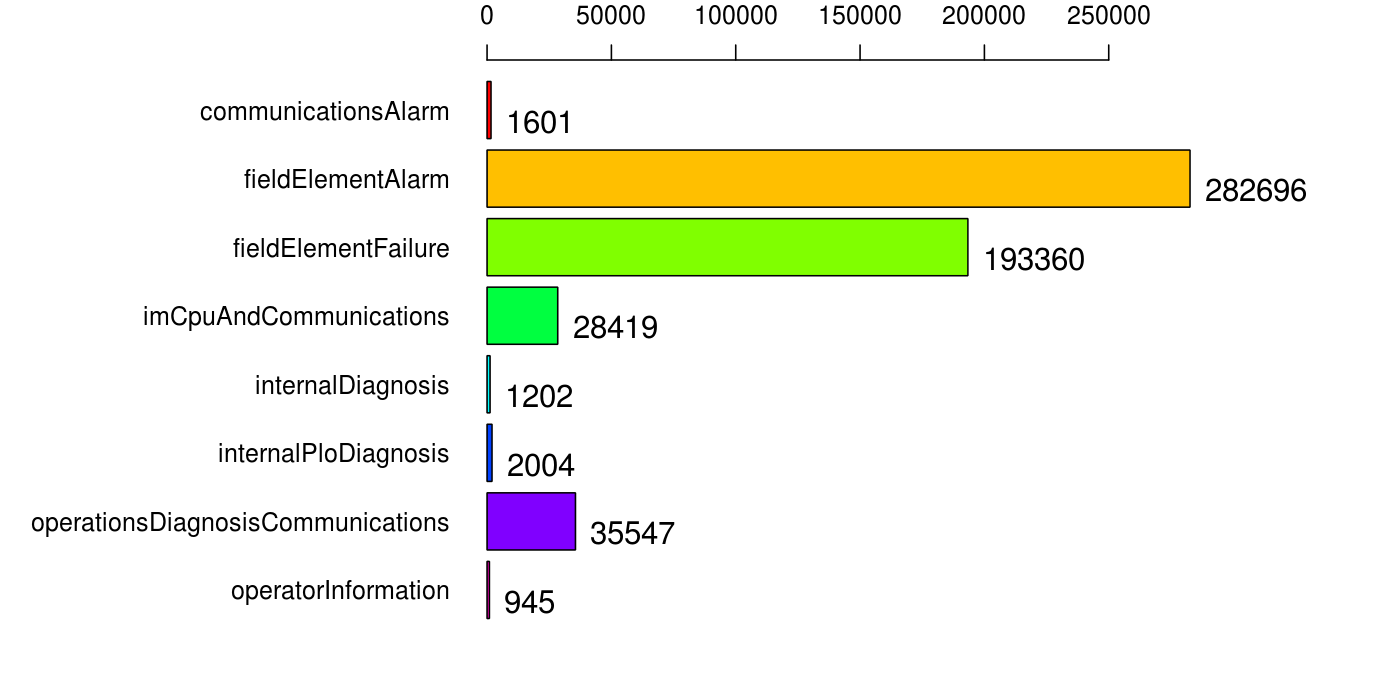
\includegraphics[width=\textwidth]{img/clusters_alb.png}
\caption{Clusters and their size for Albacete station} \label{fig:clusters_alb}
\end{figure}

\begin{figure}[hbtp]
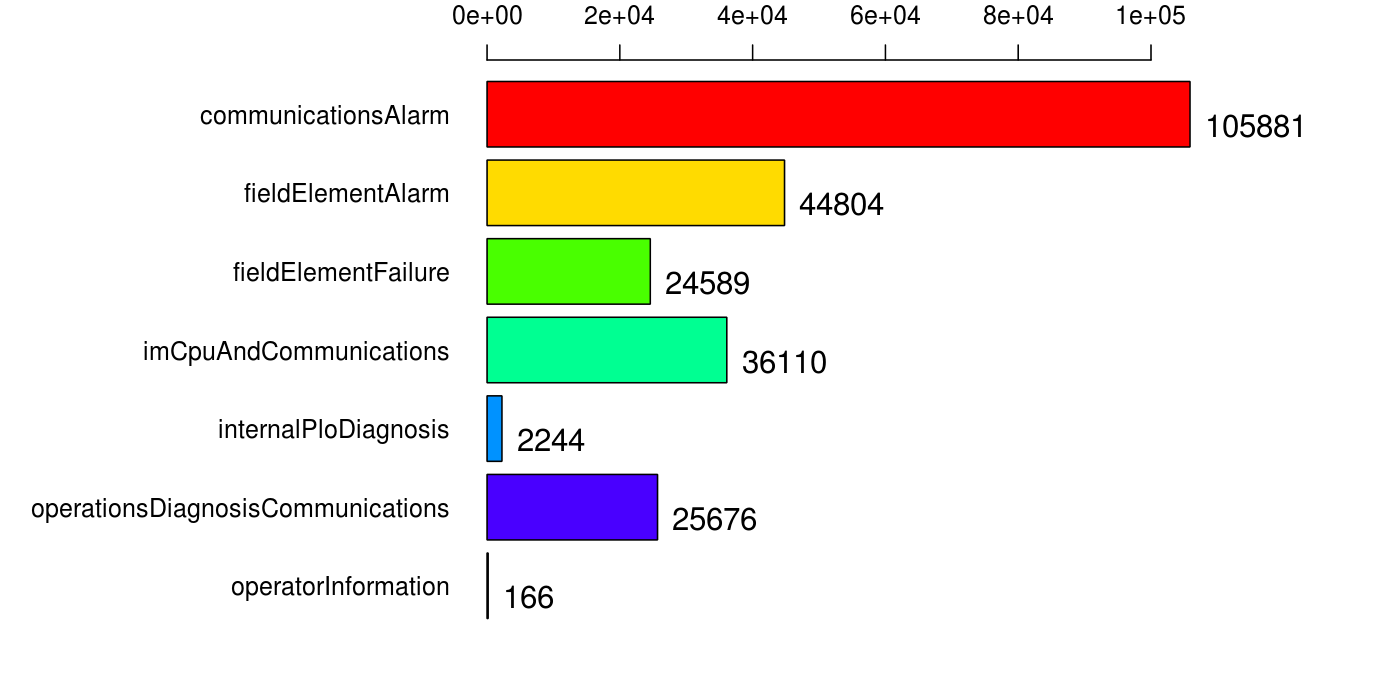
\includegraphics[width=\textwidth]{img/clusters_ant.png}
\caption{Clusters and their size for Antequera station} \label{fig:clusters_ant}
\end{figure}

\begin{figure}[hbtp]
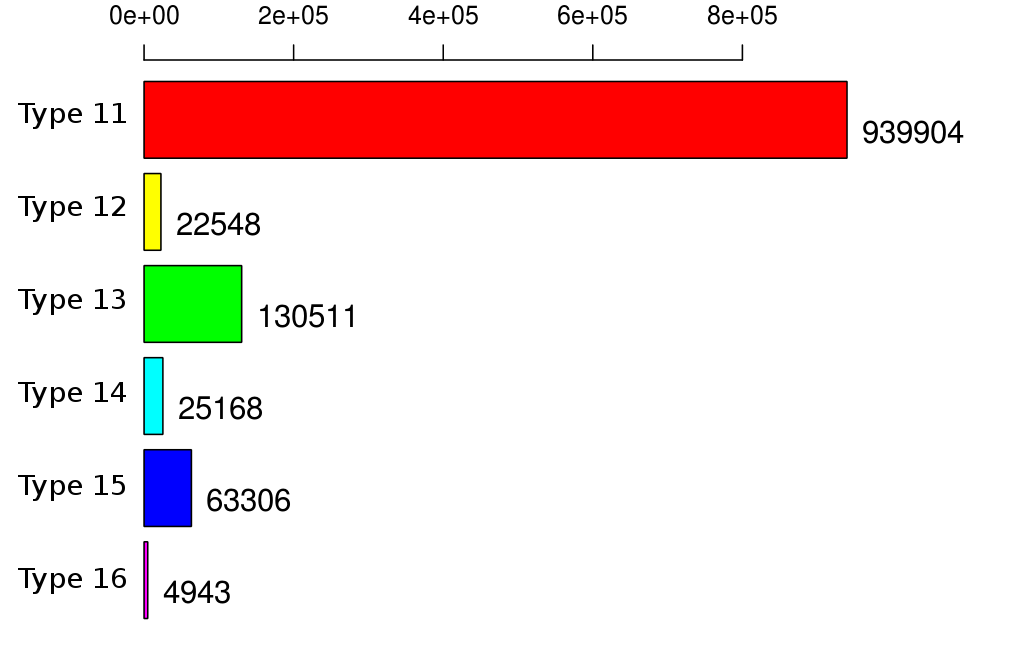
\includegraphics[width=\textwidth]{img/clusters_seg.png}
\caption{Clusters and their size for Segovia station} \label{fig:clusters_seg}
\end{figure}

\begin{figure}[hbtp]
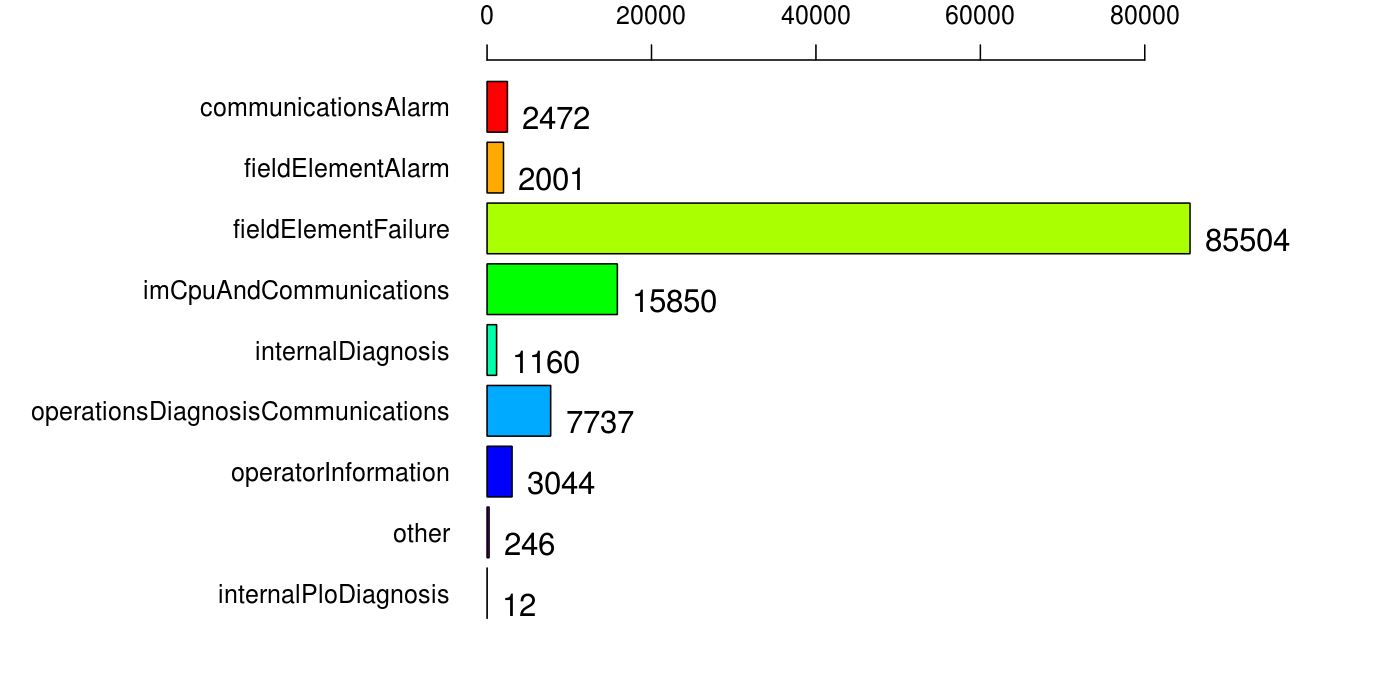
\includegraphics[width=\textwidth]{img/clusters_sev.png}
\caption{Clusters and their size for Sevilla station} \label{fig:clusters_sev}
\end{figure}


\begin{table}
\begin{center}
\begin{tabular}{|c|c|c|}
\hline \headcell{Cluster size} & \headcell{Maximum number of antecedents} & \headcell{Minimum support} \\ 
\hline 
$<$ 10.000 & 7 & 0.01 \\ 
\hline 
10.000 - 50.000 & 5 & 0.1 \\ 
\hline 
50.000 - 100.000 & 5 & 0.2 \\ 
\hline 
$>$100.000 & 5 & 0.3 \\ 
\hline 

\end{tabular} 
\caption{Search depth parameters for different cluster sizes} \label{tab:thumbrule}
\end{center}
\end{table}

\subsection{Grouping similar physical elements}
\label{sec:group_elements}
As a second method, we will try and group alarms by the element which raises them. For our \emph{empty intersection} rule to be followed, we will need to make groups which gather \emph{all} the elements which can raise the same type of alarms. Unfortunately, information on the physical elements which raise the alarms is not directly tabulated and available in the provided databases. The corresponding element is instead included as part of the message shown to the operator, sometimes along with other parameters, and therefore this classification cannot be directly made.

In order to achieve this, we will check, for all the different possible events, their associated \emph{ADDITIONAL\_INFOS} field, which depends on (but not corresponds to) the raising elements. By looking for similar naming patterns on said field, we might be able to find a way to perform this desired way of clustering. Most of the groups did not follow evident patterns at first sight, but after analysing all their relations with different alarms, we were able to come with several clusters. The created groups for Antequera station can be seen in table~\ref{tab:custom_clusters}. For example, \emph{ADDITIONAL\_INFOS} fields of the form E1, E2, E3... always were found in lights-related alarms, same as for the form R1, R2, R3... and therefore all the events falling into these conditions will be clustered into the \emph{lights} cluster.

These groups do not follow any official categorisation made by Thales' engineers. Although an index of physical elements existed and was available, its relation with the alarms in the database was not direct. Furthermore, what we want to achieve is groups of elements which are likely to raise similar elements (and to follow similar patterns in their occurence) and therefore we do not need these groups to be actually made by exact classification of the types of elements.

Comparison of results with and without this kind of clustering can be seen in figure~\ref{fig:group_vs_nogroup}. The number of high-precision rules significantly increases by using this kind of clustering. Further comments on the results can be found in section~\ref{sec:results}.

This process, however, must be made manually looking for different patterns and elements which seem to raise the same type of events. Therefore, it is a very time consuming process and its not suitable for being applied systematically to all datasets. The provided data corresponds to the station of Antequera, for which we have performed the procedure in order to evaluate its possible benefits. In order for this to be suitable for general application, additional info should be provided in datasets which could allow faster automatic grouping.

\begin{table}
\begin{center}
\begin{tabular}{|c|c|c|}
\hline \headcell{ADDITIONAL\_INFOS pattern} & \headcell{Cluster} \\ 
\hline 
A00, A01, A02... & Switches \\ 
\hline 
10, 11, 12... 140 & Lights \\ 
\hline 
E1, E2, E3, E4 ... & Lights \\ 
\hline 
S1/1, S1/2 ... & Lights \\ 
\hline 
R1, R2, R3 ... & Lights \\ 
\hline 
M1, M2, M3 ... & Lights \\ 
\hline 
A|XX|XX & Communications \\ 
\hline 
B|XX|XX & Communications \\ 
\hline 
IM|XX|XX & Communications \\ 
\hline 
EC|XX|XX & Communications \\ 
\hline
EN-A, EN-B, EN-M & Electric network and power supply \\ 
\hline   
ALI\_XXX & Electric network and power supply \\ 
\hline   
Alimentacion XXX & Electric network and power supply \\ 
\hline   
V1, V2 ... & Rail tracks \\ 
\hline   

\end{tabular} 
\caption{Clusters found for different patterns in ADDITIONAL\_INFOS field} \label{tab:custom_clusters}
\end{center}
\end{table}

\begin{figure}[hbtp]
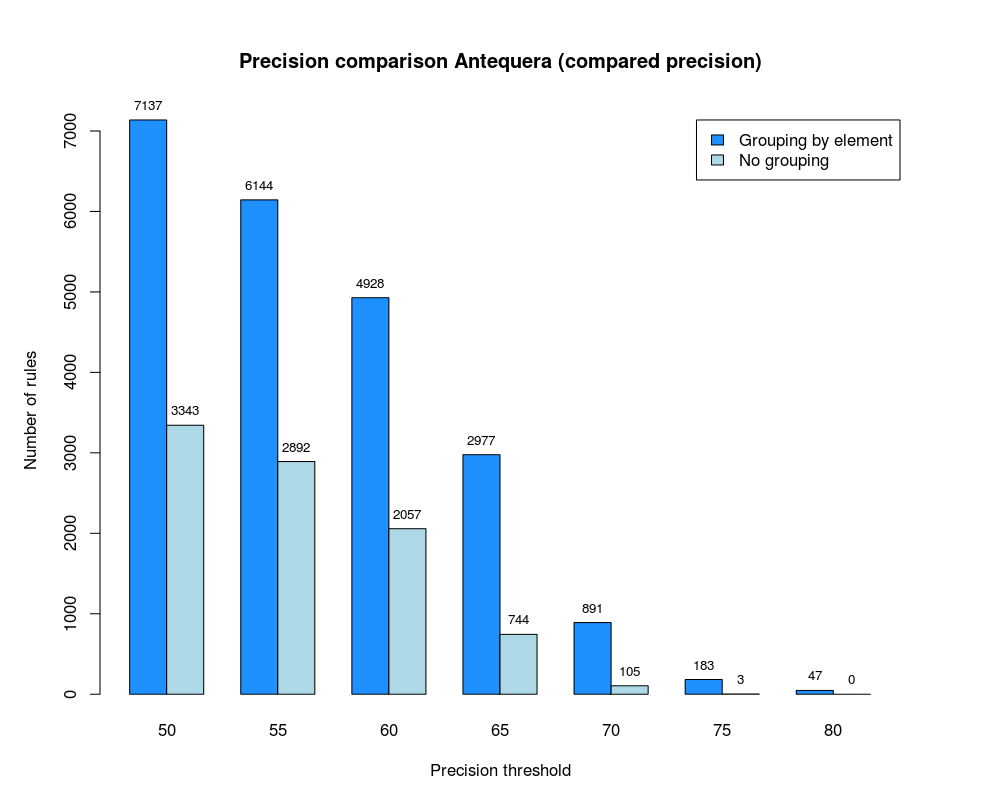
\includegraphics[width=\textwidth]{img/group_vs_nogroup.png}
\caption{Number of rules by precision before and after grouping by similar elements} \label{fig:group_vs_nogroup}
\end{figure}

\clearpage
\section{Results}
\label{sec:results}
In this section we will make a deep insight on the obtained data. Our goal was to generate different rulesets for each of our maintenance stations, each of them covering different time windows. Specifically, we have studied three different time windows: one day, two days and one week. This defines the observation period for our predictive work, which means not only the time span we will use as antecedents for our rules but also the time window within which our prediction can occur.

The results are very different depending on which station and time period we chose. In this section we will analyse the results obtained for each of them from different perspectives.

\subsection{Description of obtained rulesets}
\label{sec:desc_results}
The result of the previous work described in section~\ref{sec:assoc_rules} comes in the form of a set of association rules. These \emph{rule sets} contain a list of all the association rules found, along with their performance value calculed by the \emph{K-fold-CV} procedure as defined in section~\ref{sec:validation_evaluation}. The obtained rulesets and the number of rules they contain can be seen in table~\ref{tab:numrules}.

These sets contain all the information obtained from the procedure defined in section~\ref{sec:assoc_rules}. It is important to note that not all of them will be useful in order to implement a predictive system, as their precision is sometimes as low as 5\%. The threshold for a rule to be useful needs to be defined by maintenance workers who know the associated costs of maintenance tasks required to handle raised predictions before knowing if they will actually happen. If some event needs a significantly high amount of money to be avoided we will probably want to be \emph{very} confident about our precisions regarding that kind of event before investing resources on preventing it.

However, in general terms we can consider a prediction is good when it has more chances of being a right guess than a wrong one. We will therefore set p=0.5 as the point where rules \emph{start} to be useful. Rules with lower precisions are still provided and can be useful for other analysis tasks or further research, but from now on we will disregard them and focus on the \emph{0.5 set} which can be used right away for predictive purposes. These new sets and their size can be seen in table~\ref{tab:numrules_50}. Obviously, the size of the sets reduces drastically when imposing this kind of conditions.

\begin{table}
\begin{center}
\begin{tabular}{|c|c|c|}
\hline \headcell{Station} & \headcell{Time Window} & \headcell{Rules} \\ 
\hline 
Albacete & 1 day & 27522 \\ 
\hline 
Albacete & 7 days & 50281 \\ 
\hline 
Antequera & 1 day & 39214 \\ 
\hline 
Segovia & 1 day & 113 \\ 
\hline 
Segovia & 2 days & 72 \\ 
\hline
Segovia & 7 days & 133 \\ 
\hline 
Sevilla & 1 day & 8091 \\ 
\hline 

\end{tabular} 
\caption{Size of obtained rule sets for each station and time window} \label{tab:numrules}
\end{center}
\end{table}

\begin{table}
\begin{center}
\begin{tabular}{|c|c|c|}
\hline \headcell{Station} & \headcell{Time Window} & \headcell{Rules} \\ 
\hline 
Albacete & 7 days & 9 \\ 
\hline 
Antequera & 1 day & 7104 \\ 
\hline 
Segovia & 1 day & 31 \\ 
\hline 
Segovia & 2 days & 30 \\ 
\hline
Segovia & 7 days & 48 \\ 
\hline 
Sevilla & 1 day & 242 \\ 
\hline 

\end{tabular} 
\caption{Number of rules for each set setting a threshold of 50\% precision} \label{tab:numrules_50}
\end{center}
\end{table}



At this point, it is important to remember the decisions taken in terms of search depth and data subsetting as mentioned in sections~\ref{sec:search_parameters} and~\ref{sec:dataclustering}. In these terms, rule sets for some of the stations and time windows could not be generated with our available computation capabilities. A better server or algorithm optimisation would be required in order to obtain result sets for these cases.

\subsection{Number of rules against precision}
\label{sec:rules_vs_prec}
As we have seen in section~\ref{sec:desc_results}, the amount of rules decreases significantly if we impose strict conditions for their validity. In this section we will perform a deeper analysis on how amount of rules vary when setting different thresholds. For this purpose, we will set different thresholds and check the number of rules complying with this condition. The results are shown in tables \ref{tab:numrules_thresh_albacete7}, \ref{tab:numrules_thresh_antequera1}, \ref{tab:numrules_thresh_segovia1}, \ref{tab:numrules_thresh_segovia2}, \ref{tab:numrules_thresh_segovia7} and \ref{tab:numrules_thresh_sevilla1}. As expected, the number of rules increases exponentially when decreasing the threshold. For better visualization, these amounts for the \emph{$>50\%$ subsets} are represented in figures~\ref{fig:precision_alb7}, \ref{fig:precision_ant1}, \ref{fig:precision_seg1}, \ref{fig:precision_seg2}, \ref{fig:precision_seg7} and \ref{fig:precision_sev1}.

\begin{table}
\begin{center}
\begin{tabular}{|c|c|c|}
\hline \headcell{Threshold} & \headcell{Number of rules} \\ 
\hline 
0.05 & 44620 \\ 
\hline 
0.10 & 38007 \\ 
\hline 
0.20 & 4060 \\ 
\hline 
0.30 & 30 \\ 
\hline
0.40 & 27 \\ 
\hline 
0.50 & 9 \\ 
\hline 
0.60 & 8 \\ 
\hline 

\end{tabular} 
\caption{Number of rules for different thresholds in Albacete (7 days)} \label{tab:numrules_thresh_albacete7}
\end{center}
\end{table}

\begin{table}
\begin{center}
\begin{tabular}{|c|c|c|}
\hline \headcell{Threshold} & \headcell{Number of rules} \\ 
\hline 
0.05 & 31846 \\ 
\hline 
0.10 & 28338 \\ 
\hline 
0.20 & 21566 \\ 
\hline 
0.30 & 15829 \\ 
\hline
0.40 & 10876 \\ 
\hline 
0.50 & 7137 \\ 
\hline 
0.60 & 4928 \\ 
\hline 
0.70 & 891 \\ 
\hline 
0.80 & 47 \\ 
\hline 

\end{tabular} 
\caption{Number of rules for different thresholds in Antequera (1 day)} \label{tab:numrules_thresh_antequera1}
\end{center}
\end{table}

\begin{table}
\begin{center}
\begin{tabular}{|c|c|c|}
\hline \headcell{Threshold} & \headcell{Number of rules} \\ 
\hline 
0.05 & 106 \\ 
\hline 
0.10 & 95 \\ 
\hline 
0.20 & 72 \\ 
\hline 
0.30 & 44 \\ 
\hline
0.40 & 33 \\ 
\hline 
0.50 & 31 \\ 
\hline 
0.60 & 30 \\ 
\hline 
0.70 & 24 \\ 
\hline 
0.80 & 12 \\ 
\hline 

\end{tabular} 
\caption{Number of rules for different thresholds in Segovia (1 day)} \label{tab:numrules_thresh_segovia1}
\end{center}
\end{table}

\begin{table}
\begin{center}
\begin{tabular}{|c|c|c|}
\hline \headcell{Threshold} & \headcell{Number of rules} \\ 
\hline 
0.05 & 69 \\ 
\hline 
0.10 & 66 \\ 
\hline 
0.20 & 56 \\ 
\hline 
0.30 & 40 \\ 
\hline
0.40 & 31 \\ 
\hline 
0.50 & 30 \\ 
\hline 
0.60 & 14 \\ 
\hline 

\end{tabular} 
\caption{Number of rules for different thresholds in Segovia (2 days)} \label{tab:numrules_thresh_segovia2}
\end{center}
\end{table}

\begin{table}
\begin{center}
\begin{tabular}{|c|c|c|}
\hline \headcell{Threshold} & \headcell{Number of rules} \\ 
\hline 
0.05 & 128 \\ 
\hline 
0.10 & 125 \\ 
\hline 
0.20 & 92 \\ 
\hline 
0.30 & 75 \\ 
\hline
0.40 & 64 \\ 
\hline 
0.50 & 48 \\ 
\hline 
0.60 & 35 \\ 
\hline 
0.70 & 30 \\ 
\hline 
0.80 & 25 \\ 
\hline 
0.90 & 4 \\ 
\hline 

\end{tabular} 
\caption{Number of rules for different thresholds in Segovia (7 days)} \label{tab:numrules_thresh_segovia7}
\end{center}
\end{table}

\begin{table}
\begin{center}
\begin{tabular}{|c|c|c|}
\hline \headcell{Threshold} & \headcell{Number of rules} \\ 
\hline 
0.05 & 6730 \\ 
\hline 
0.10 & 2832 \\ 
\hline 
0.20 & 2357 \\ 
\hline 
0.30 & 1799 \\ 
\hline
0.40 & 642 \\ 
\hline 
0.50 & 246 \\ 
\hline 
0.60 & 78 \\ 
\hline 
0.70 & 2 \\ 
\hline 

\end{tabular} 
\caption{Number of rules for different thresholds in Sevilla (1 day)} \label{tab:numrules_thresh_sevilla1}
\end{center}
\end{table}

\begin{figure}[hbtp]
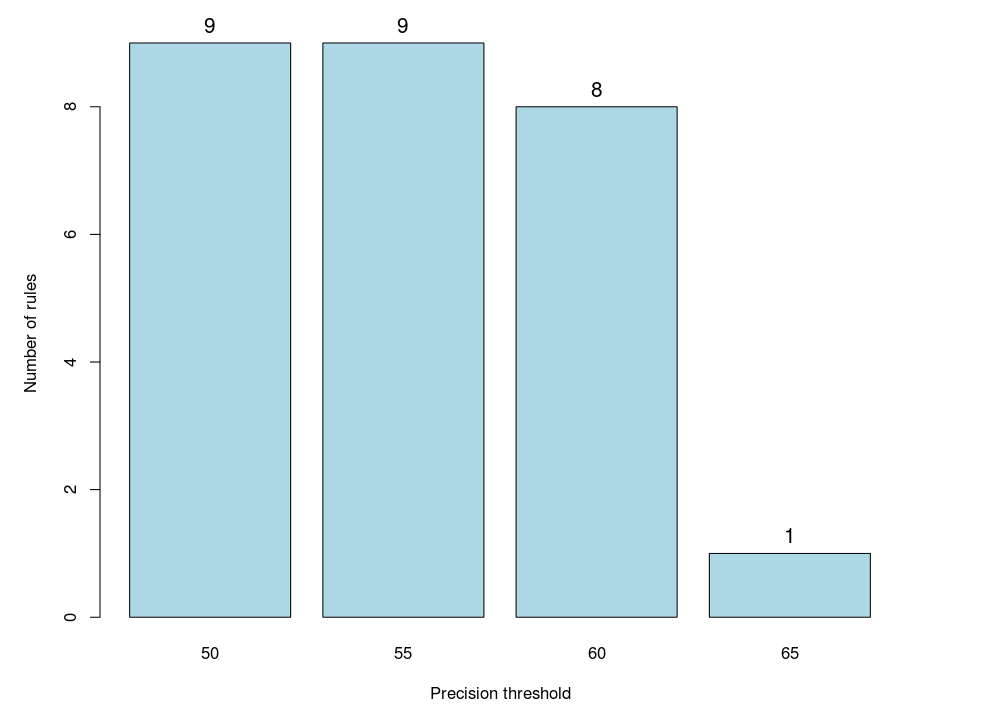
\includegraphics[width=\textwidth]{img/precision_alb7.png}
\caption{Number of rules for different thresholds in Albacete (7 days)} \label{fig:precision_alb7}
\end{figure}

\begin{figure}[hbtp]
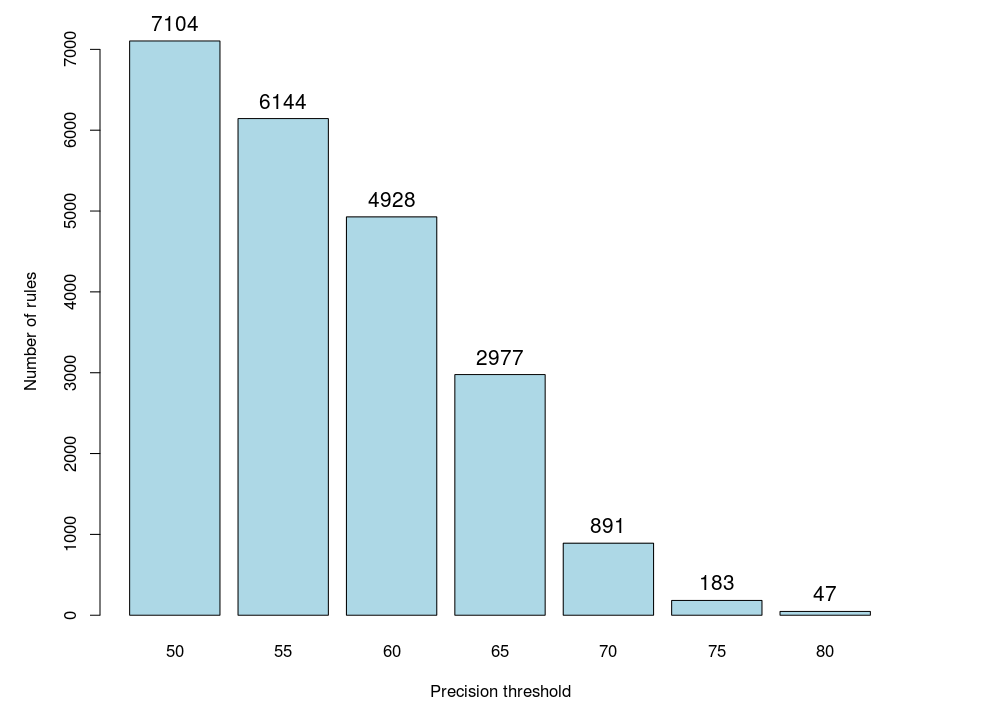
\includegraphics[width=\textwidth]{img/precision_ant1.png}
\caption{Number of rules for different thresholds in Antequera (1 day)} \label{fig:precision_ant1}
\end{figure}

\begin{figure}[hbtp]
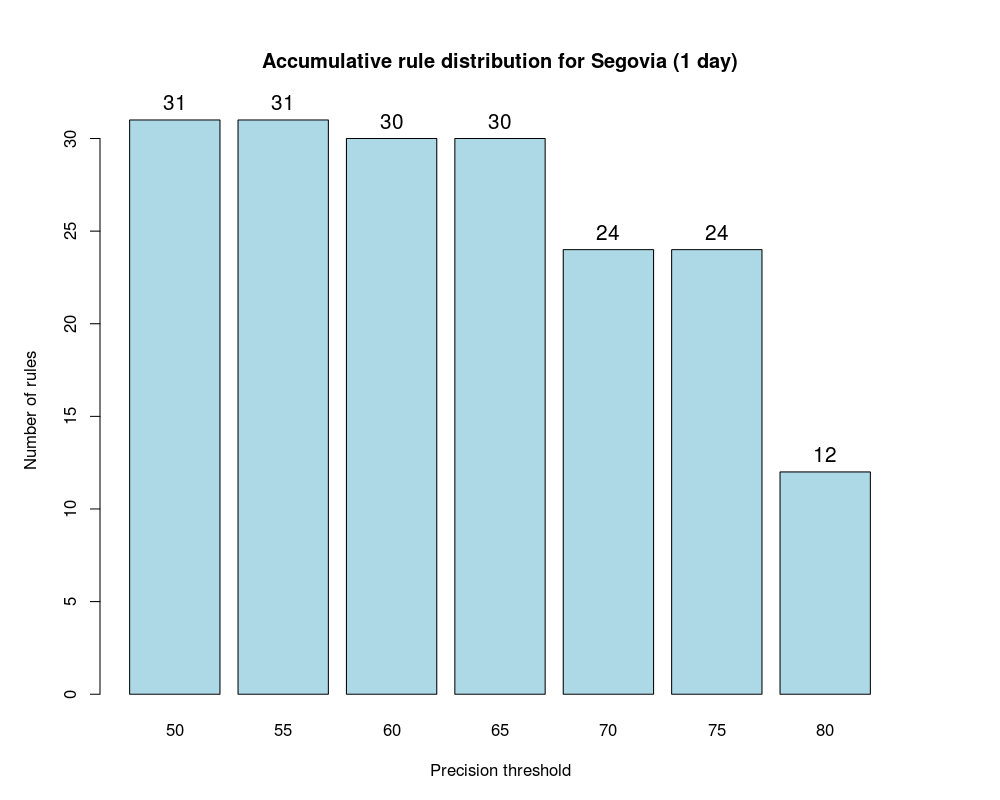
\includegraphics[width=\textwidth]{img/precision_seg1.png}
\caption{Number of rules for different thresholds in Segovia (1 day)} \label{fig:precision_seg1}
\end{figure}

\begin{figure}[hbtp]
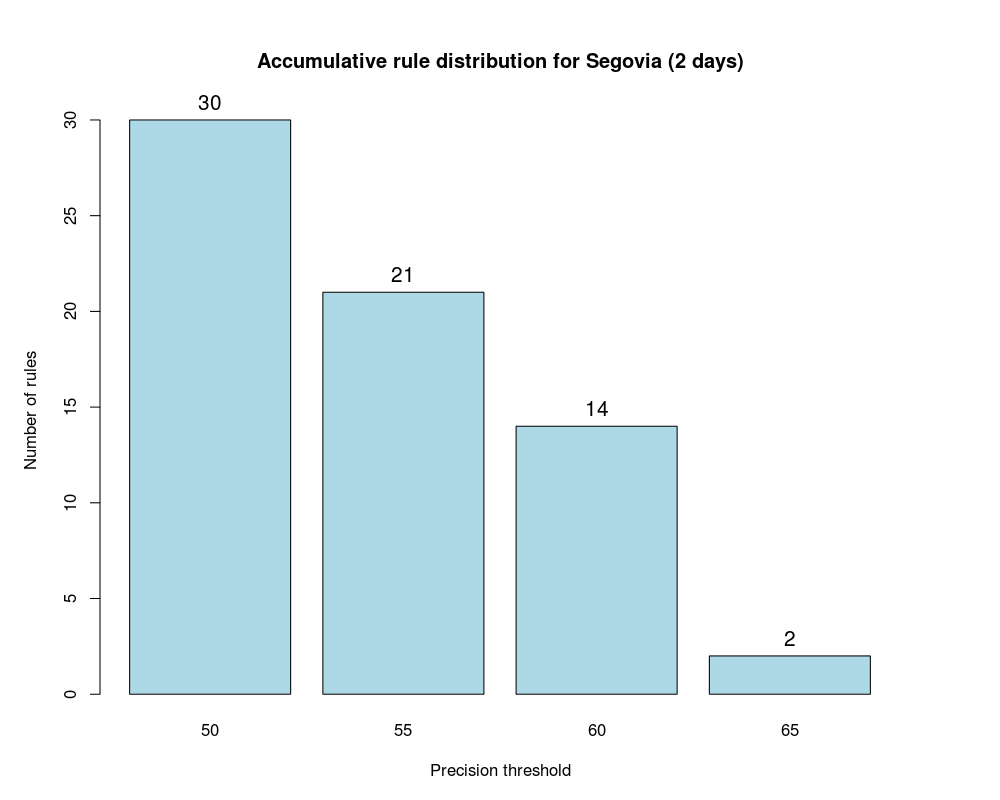
\includegraphics[width=\textwidth]{img/precision_seg2.png}
\caption{Number of rules for different thresholds in Segovia (2 days)} \label{fig:precision_seg2}
\end{figure}

\begin{figure}[hbtp]
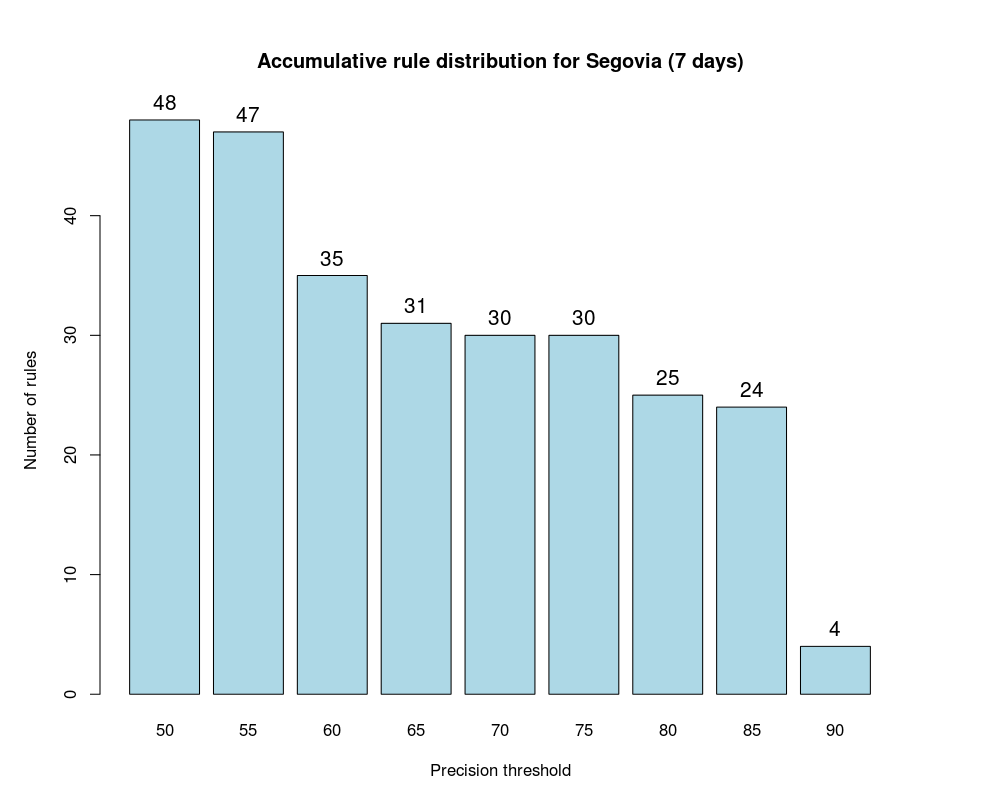
\includegraphics[width=\textwidth]{img/precision_seg7.png}
\caption{Number of rules for different thresholds in Segovia (7 days)} \label{fig:precision_seg7}
\end{figure}

\begin{figure}[hbtp]
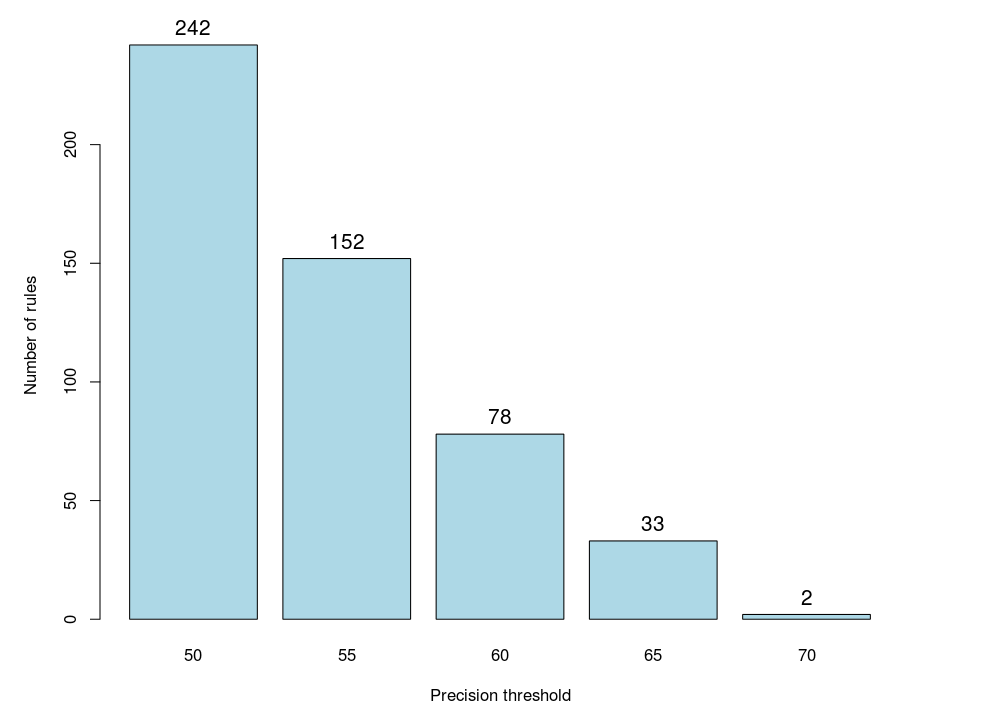
\includegraphics[width=\textwidth]{img/precision_sev1.png}
\caption{Number of rules for different thresholds in Sevilla (1 day)} \label{fig:precision_sev1}
\end{figure}

\clearpage

\subsection{Precision distribution}
\label{sec:precision_distribution}
In section~\ref{sec:rules_vs_prec} we analysed the number of rules we would obtain if we set different precision levels as thresholds to generate different subsets. According to our expectations, we observed a decay in these numbers as we set higher thresholds. However, this decay, although apparently exponential, shows flat zones and other irregularities which would be unexpected at first.

In order to better visualize these anomalities we will graphically represent the precision distribution in form of histograms for the previous sets. These distributions can be seen in figures~\ref{fig:hist_alb7}, \ref{fig:hist_ant1}, \ref{fig:hist_seg1}, \ref{fig:hist_seg2}, \ref{fig:hist_seg7} and \ref{fig:hist_sev1}.

In these histograms we can see that the distribution does not grow exponentially as we lower the precision, as we would expect and as we apparently saw in the analysis from section~\ref{sec:rules_vs_prec}. Instead, there are some accumulation points around which precision tends to take values. 

For example, looking at the distribution for Antequera (figure~\ref{fig:hist_ant1}) we see that there are more rules with precisions between 0.65 and 0.70 than between 0.50 and 0.55.

As we do not have large sets of rules for all the stations, performing a deeper analysis of the distributions is not possible. As these kind of irregularities appear for all the studied cases, it is very unlikely that they are caused just by chance. However, the causes and possible implications of these distributions cannot be infered at this point and would require further research.

\begin{figure}[hbtp]
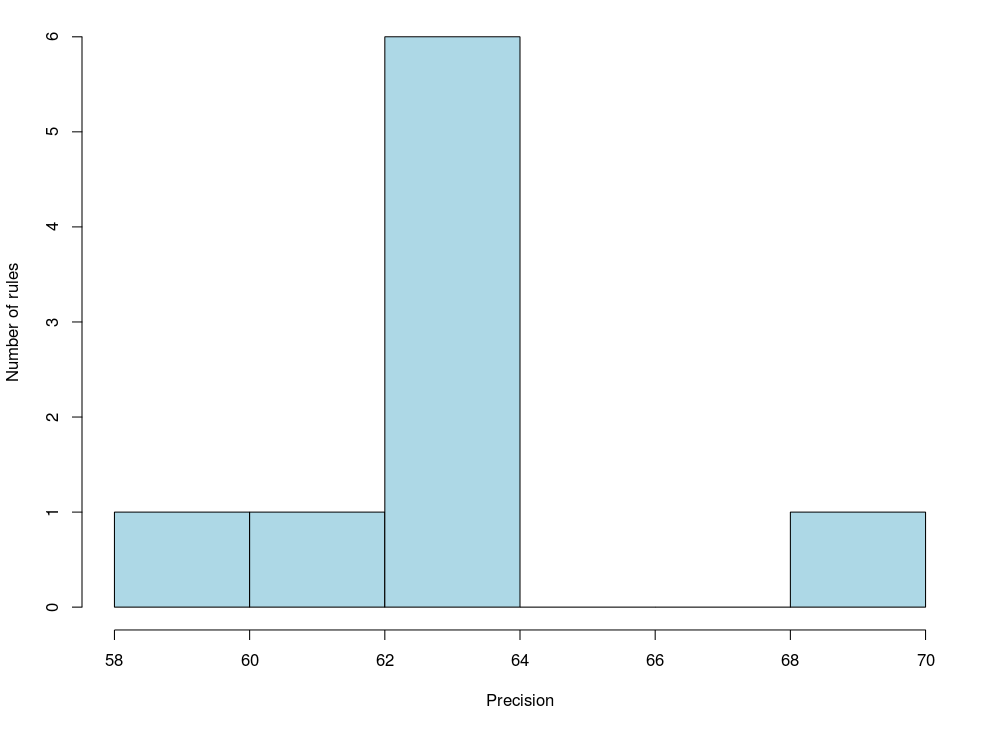
\includegraphics[width=\textwidth]{img/hist_alb7.png}
\caption{Rule distribution by precision in Albacete (7 days)} \label{fig:hist_alb7}
\end{figure}

\begin{figure}[hbtp]
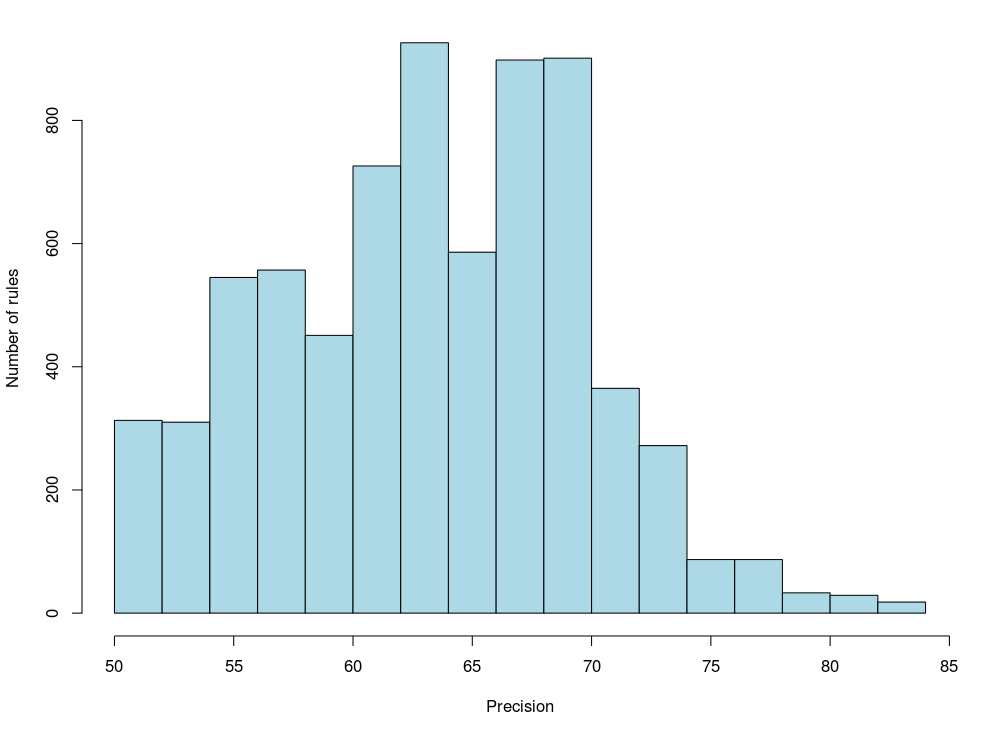
\includegraphics[width=\textwidth]{img/hist_ant1.png}
\caption{Rule distribution by precision in Antequera (1 day)} \label{fig:hist_ant1}
\end{figure}

\begin{figure}[hbtp]
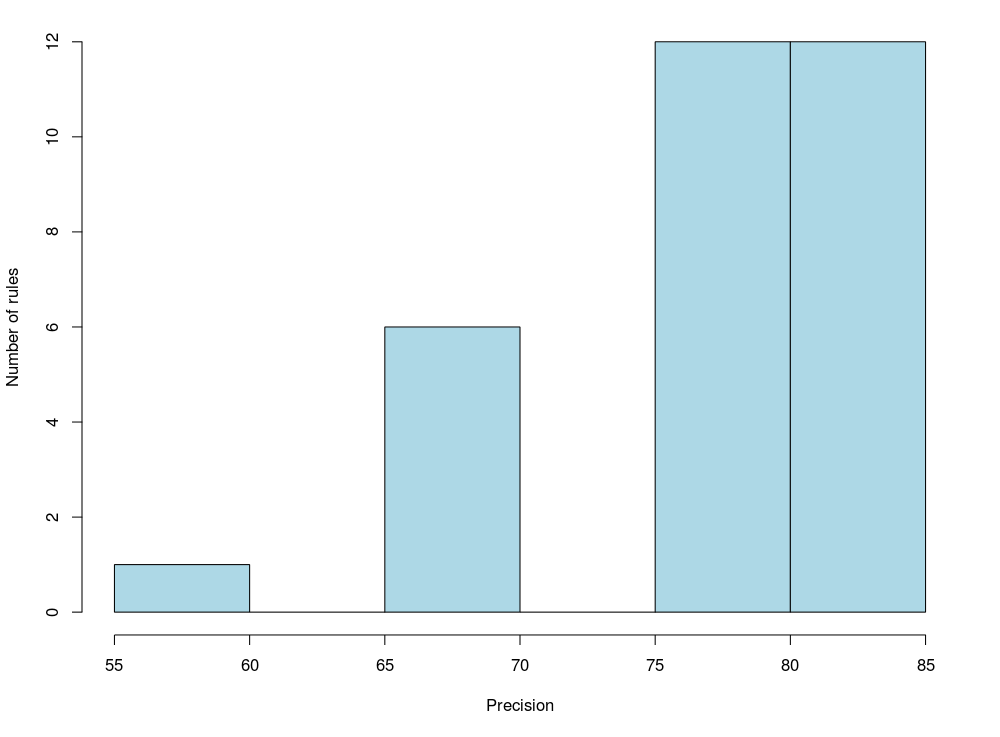
\includegraphics[width=\textwidth]{img/hist_seg1.png}
\caption{Rule distribution by precision in Segovia (1 day)} \label{fig:hist_seg1}
\end{figure}

\begin{figure}[hbtp]
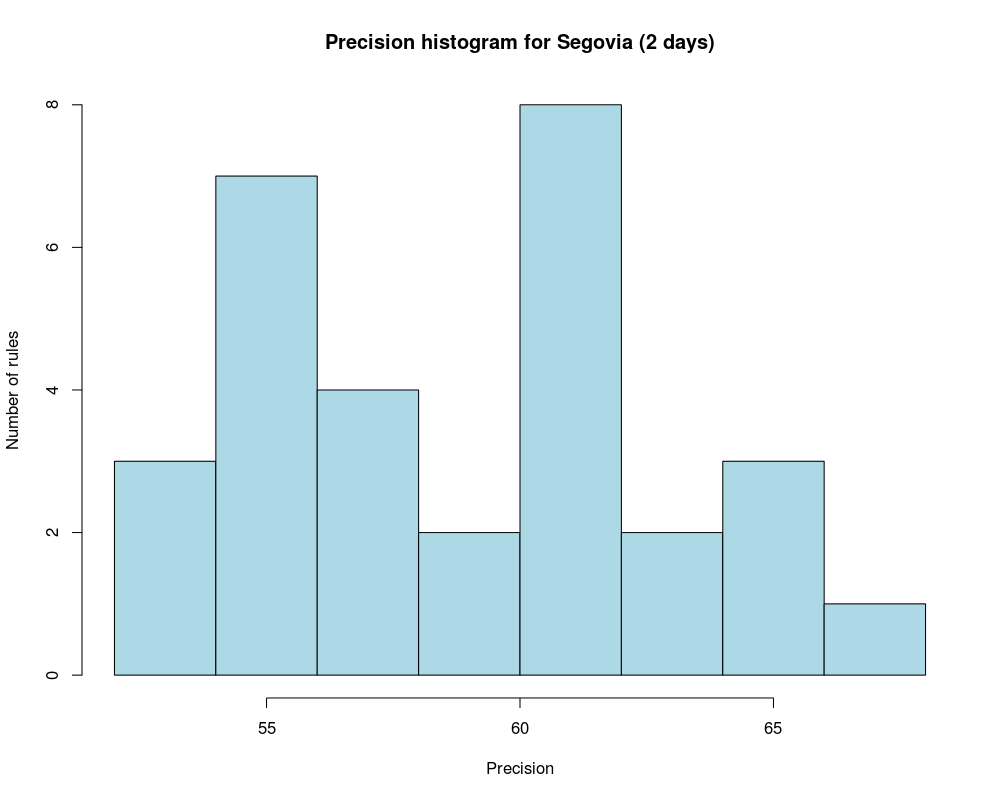
\includegraphics[width=\textwidth]{img/hist_seg2.png}
\caption{Rule distribution by precision in Segovia (2 days)} \label{fig:hist_seg2}
\end{figure}

\begin{figure}[hbtp]
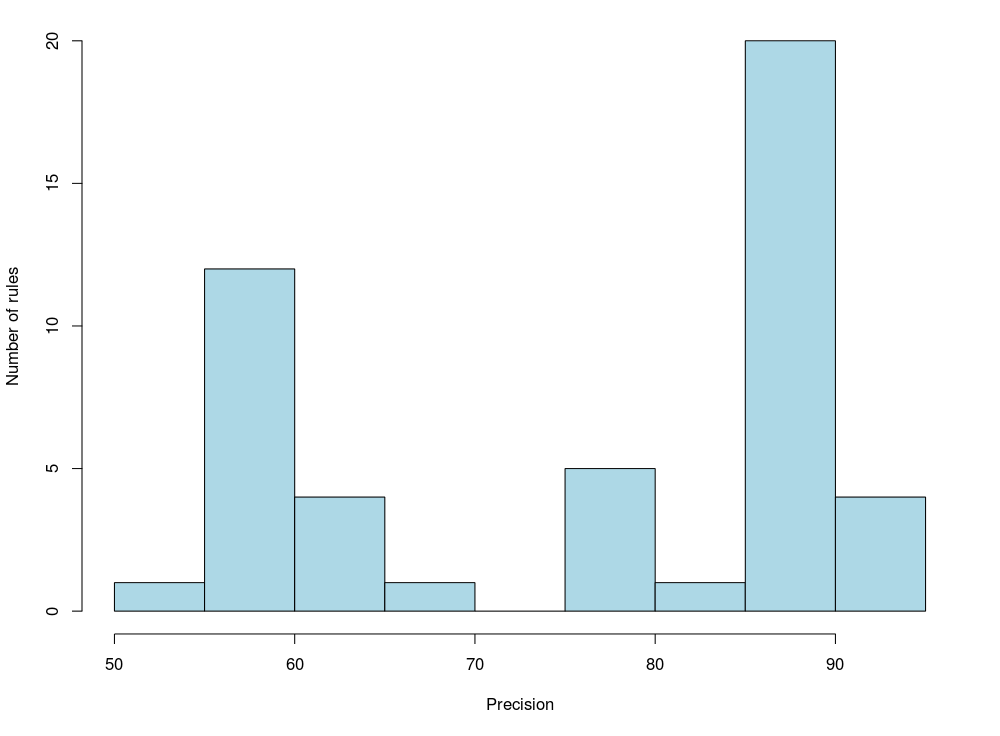
\includegraphics[width=\textwidth]{img/hist_seg7.png}
\caption{Rule distribution by precision in Segovia (7 days)} \label{fig:hist_seg7}
\end{figure}

\begin{figure}[hbtp]
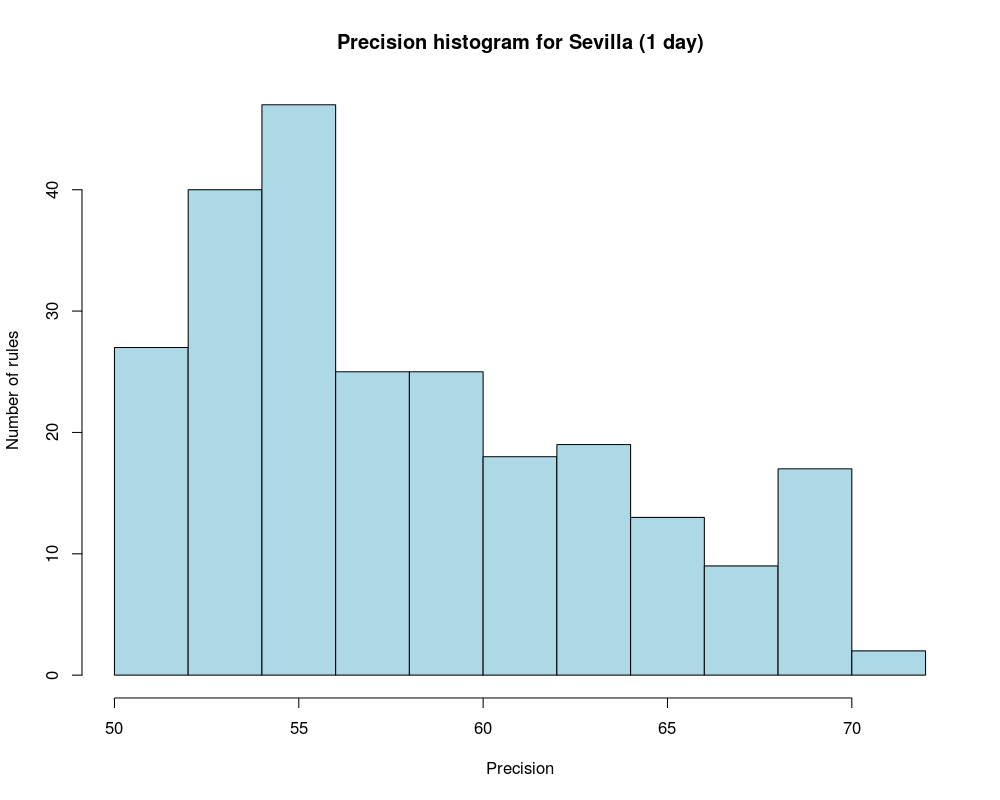
\includegraphics[width=\textwidth]{img/hist_sev1.png}
\caption{Rule distribution by precision in Sevilla (1 day)} \label{fig:hist_sev1}
\end{figure}

\subsection{Predictable events by category}
As we mentioned in section~\ref{sec:using_event_type}, one of the methods followed in order to being able to perform deep searches on our data was clustering by event types. This unavoidably leads to differences on the achievable performance for each of the different event types. This is caused not only by the different search depths which we were able to use in each of the different groups, but also by the individual nature of each of the event types: events in some of the clusters may be more likely to be related to others in the same cluster while for other types these relations may be more likely to be found to events in other clusters. 

In order to analyse the effect of this clustering in the obtained results, we will analyse the category of the events the rules predict. This is, we will analyse the event type of the consequent of our rules. This distribution can be seen in figures \ref{fig:conseqtypes_alb7}, \ref{fig:conseqtypes_ant1}, \ref{fig:conseqtypes_seg1}, \ref{fig:conseqtypes_seg2}, \ref{fig:conseqtypes_seg7} and \ref{fig:conseqtypes_sev1}.

We can see a completely uneven distribution in terms of rule generation for each event type. This is likely to be caused by two facts: nature of the events themselves (how unpredictable or related to other events they are) and frequency adequation (events which happen too often instead of only in specific situations might be harder to predict). Also, the different limit on search depth we were able to impose for the different groups also vastly affects results in this direction.

It is specially interesting the situation in \emph{Antequera}, where we performed an alternative clustering method as mentioned in \ref{sec:group_elements}. In this station, we observe that all the rules fall into the category of \emph{FieldElementFailure} and \emph{Operation diagnosis communications}. Both groups of rules are quite similar in size, although the occurence of those alarm types in the whole database is significantly different. This indicates that this kind of clustering might significantly help in order to obtain more uniform results for all the event types.

\begin{figure}[hbtp]
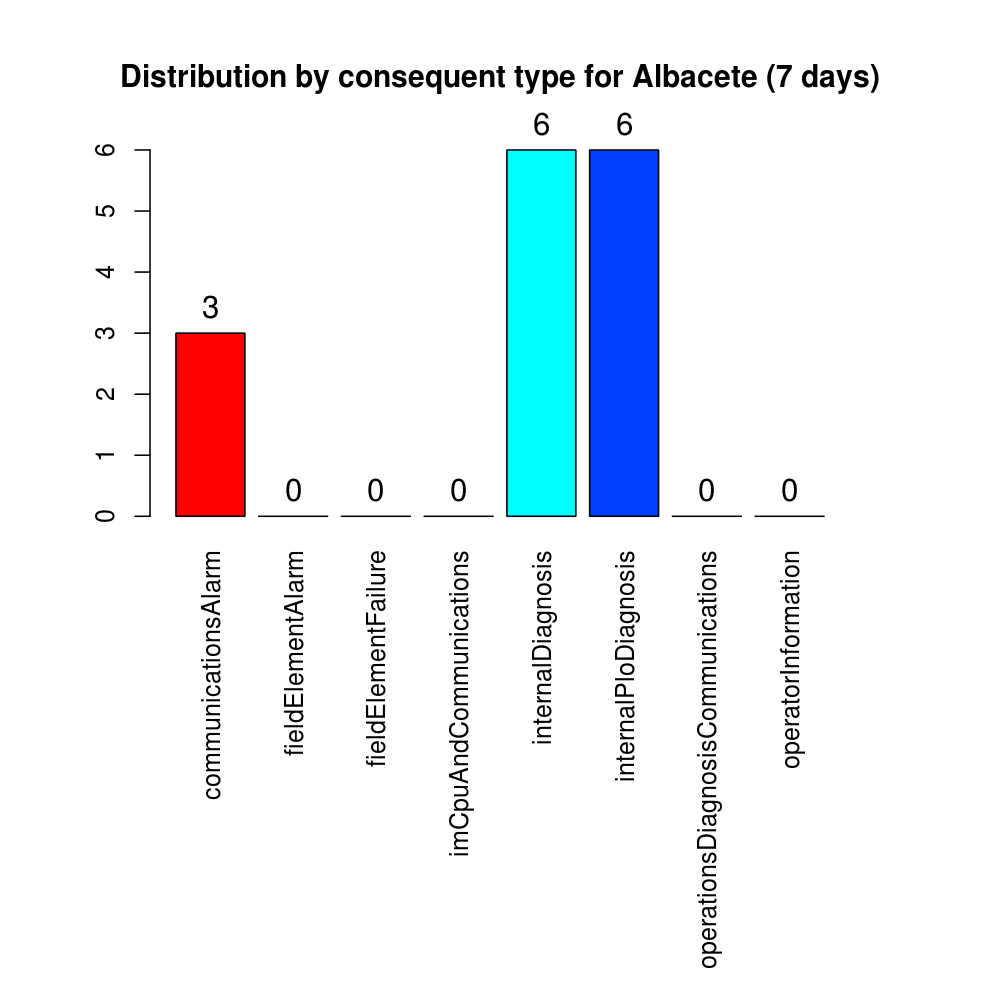
\includegraphics[width=\textwidth]{img/conseqtypes_alb7.png}
\caption{Rule distribution by consequent type in Albacete (7 days)} \label{fig:conseqtypes_alb7}
\end{figure}

\begin{figure}[hbtp]
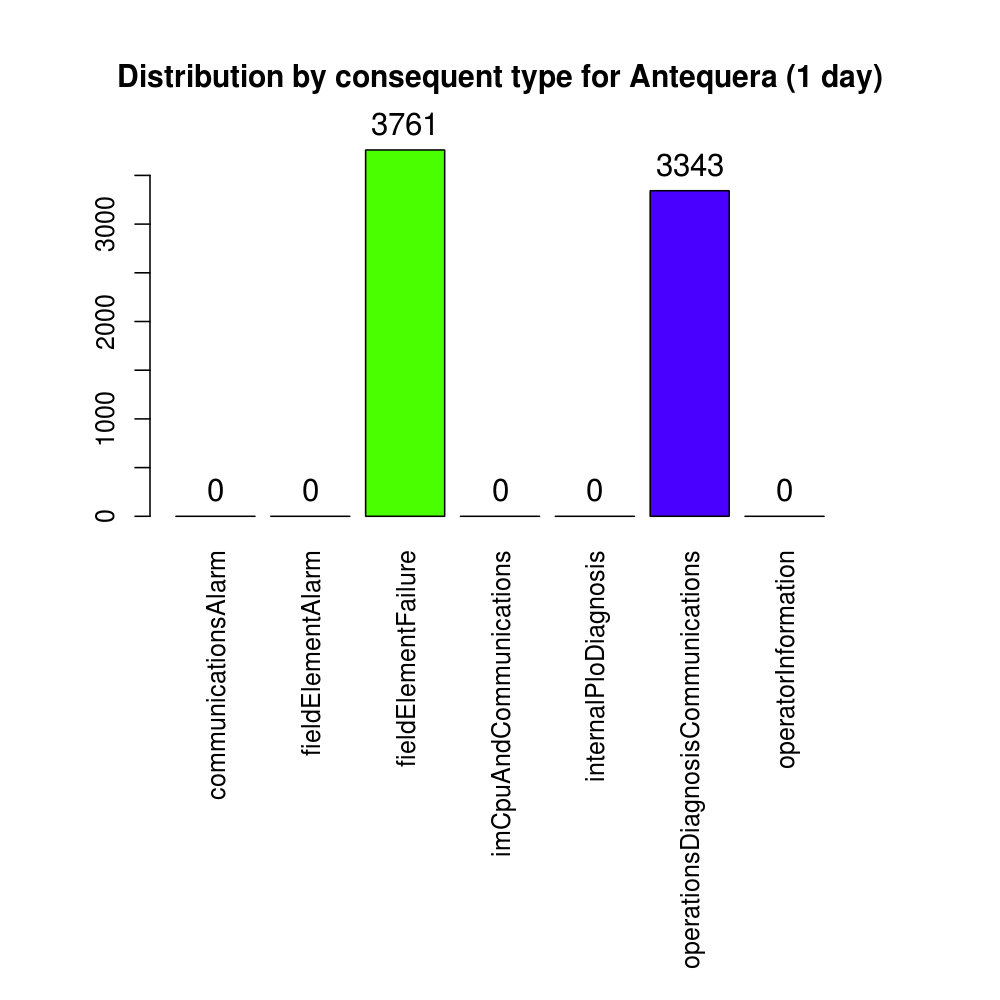
\includegraphics[width=\textwidth]{img/conseqtypes_ant1.png}
\caption{Rule distribution by consequent type in Antequera (1 day)} \label{fig:conseqtypes_ant1}
\end{figure}

\begin{figure}[hbtp]
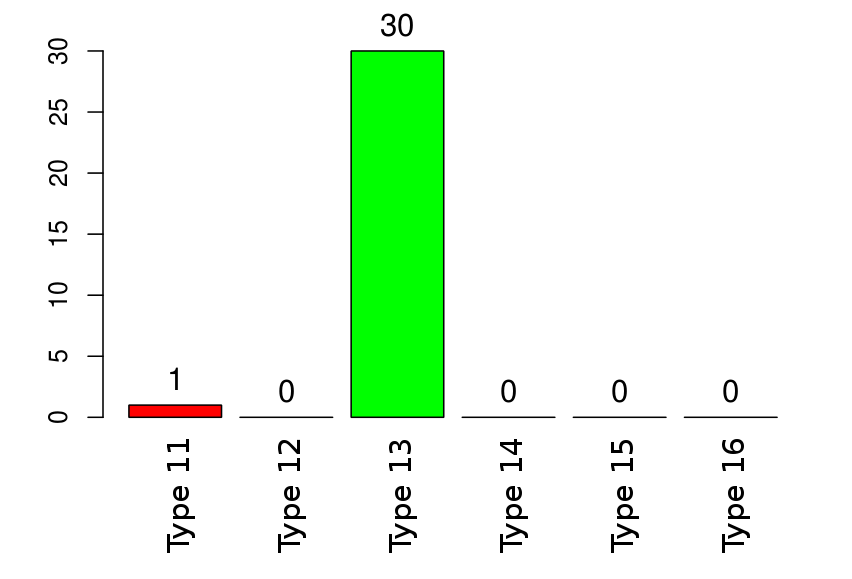
\includegraphics[width=\textwidth]{img/conseqtypes_seg1.png}
\caption{Rule distribution by consequent type in Segovia (1 day)} \label{fig:conseqtypes_seg1}
\end{figure}

\begin{figure}[hbtp]
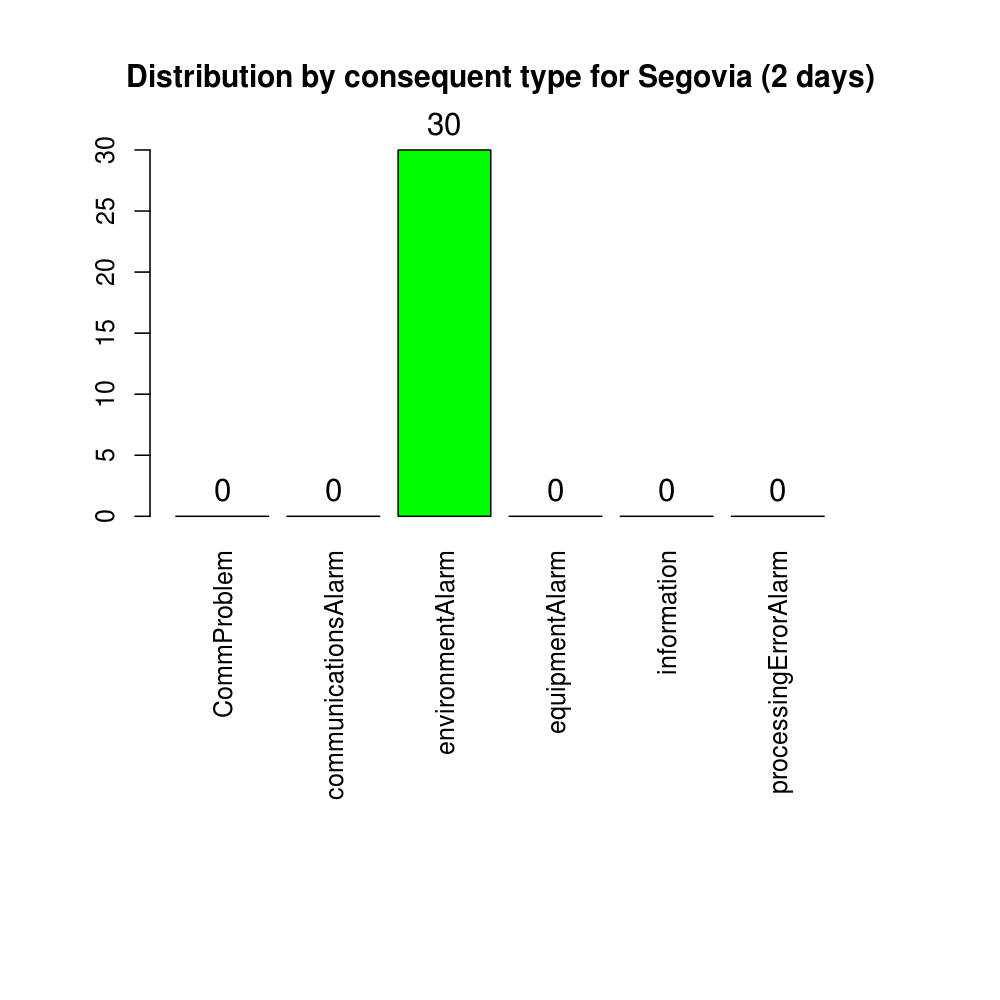
\includegraphics[width=\textwidth]{img/conseqtypes_seg2.png}
\caption{Rule distribution by consequent type in Segovia (2 days)} \label{fig:conseqtypes_seg2}
\end{figure}

\begin{figure}[hbtp]
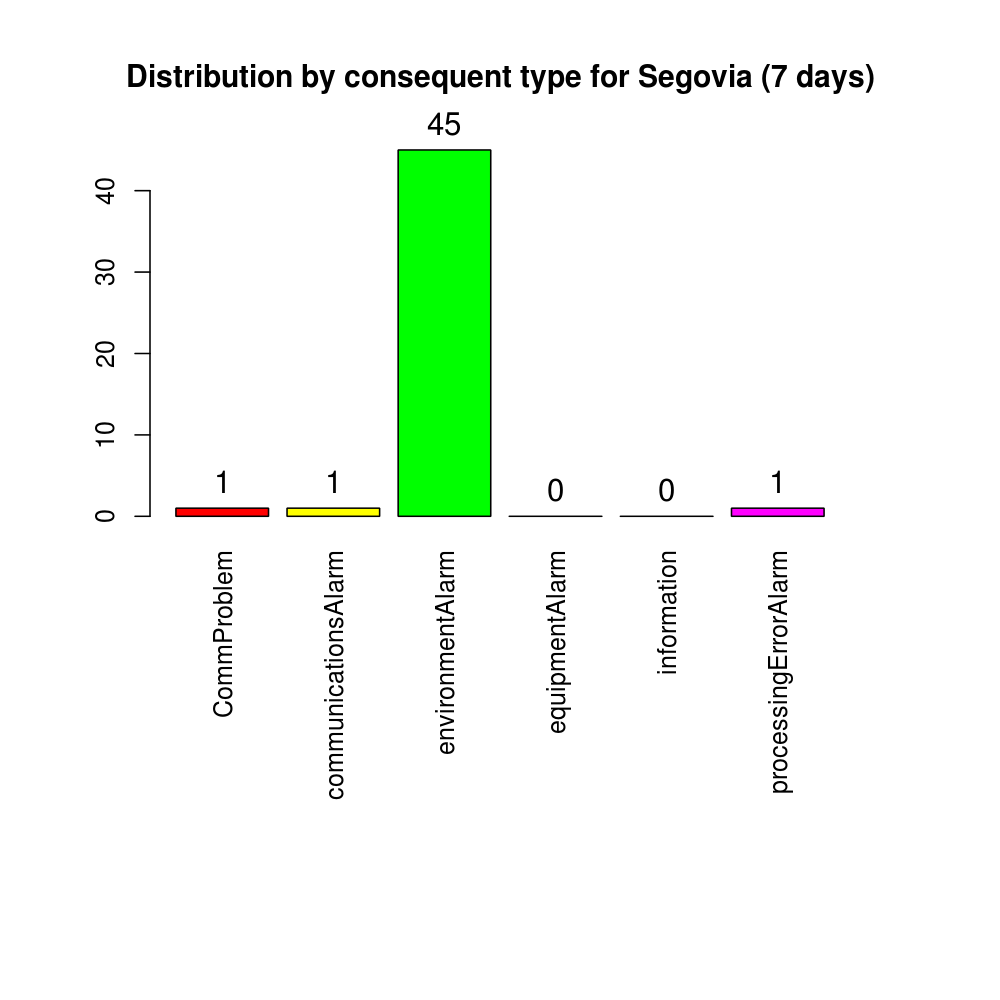
\includegraphics[width=\textwidth]{img/conseqtypes_seg7.png}
\caption{Rule distribution by consequent type in Segovia (7 days)} \label{fig:conseqtypes_seg7}
\end{figure}

\begin{figure}[hbtp]
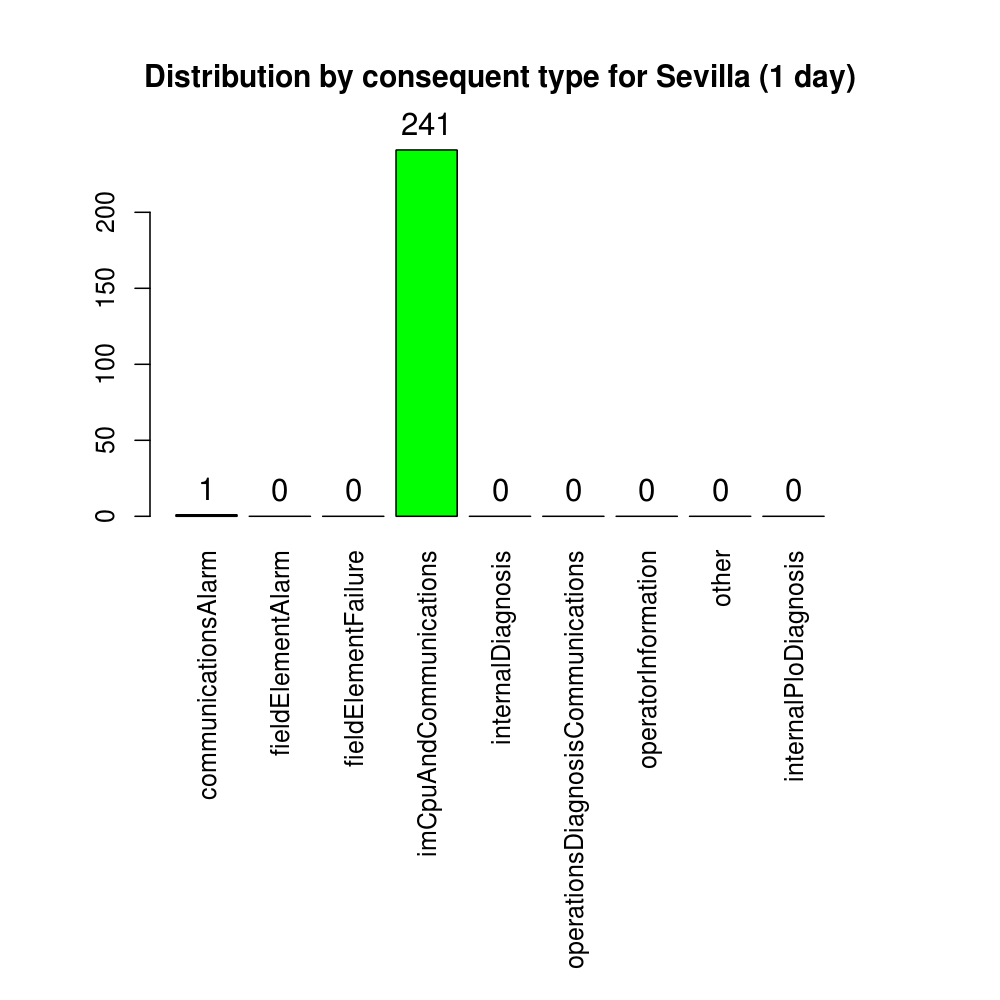
\includegraphics[width=\textwidth]{img/conseqtypes_sev1.png}
\caption{Rule distribution by consequent type in Sevilla (1 day)} \label{fig:conseqtypes_sev1}
\end{figure}


\section{Example scenario}
\label{sec:scenario}

In this section we will analyse the output of our predictive model during a short period of time. We will illustrate the kind of information an operator could obtain from an average period of time. Specifically, we will take a random period of 50 consecutive days for the station of \emph{Antequera}, over which we will perform predictions for the next days.

It is important to note that this example scenario has been obtained using the rule set with precisions higher than 0.50. In a real scenario, an operator could select a higher threshold for predictions or disregard those raised predictions with a low confidence.

\subsection{Predictions raised by event type}
First of all we will observe the number of predictions raised each day of our sample. This will give us an idea of the number of predictions our system would give for an average day. This can be seen in figure~\ref{fig:scenario_pred_categories}.

As we can see, for this station and rule set the number of predictions obtained in an average day is around 20. This does not include repeated predictions (more than one rule which can be fired simultaneously to predict the same event with different confidences).

\begin{figure}[hbtp]
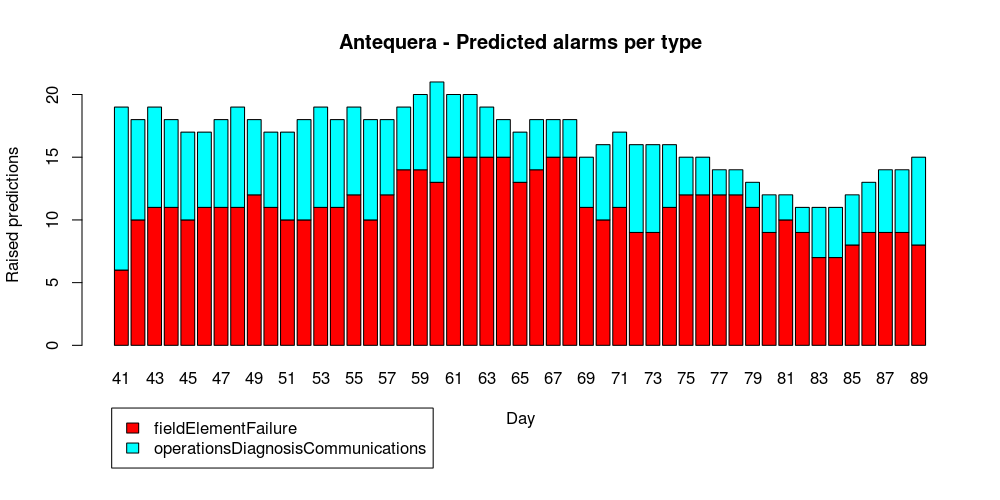
\includegraphics[width=\textwidth]{img/scenario_pred_categories.png}
\caption{Timeline of predictions during a sample period} \label{fig:scenario_pred_categories}
\end{figure}

\subsection{Percentage of events predicted}
The next thing we can analyse is the number of events which happen during an average day which are actually predicted by our system. The result is illustrated in figure~\ref{fig:scenario_pred_notpred}. This value corresponds with what we defined as \emph{recall} in section~\ref{sec:validation_evaluation}.

\begin{figure}[hbtp]
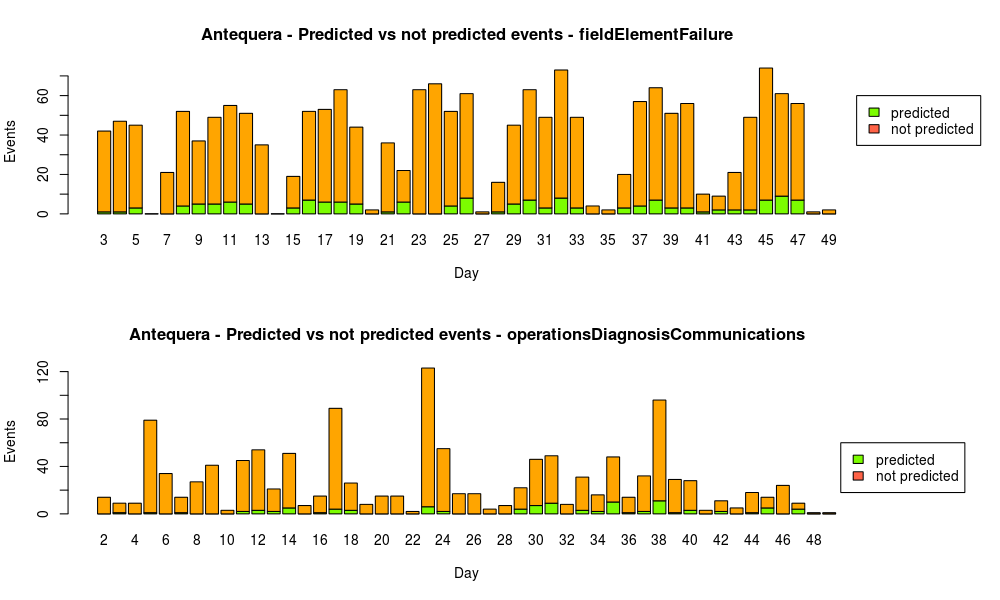
\includegraphics[width=\textwidth]{img/scenario_pred_notpred.png}
\caption{Timeline of predictions during a sample period} \label{fig:scenario_pred_notpred}
\end{figure}

\subsection{Percentage of right predictions}
To end with, we will analyse how many of the raised predictions are actually true. In order to illustrate better this aspect and take into account also the confidence parameter of the predictions, we will perform three different analysis: one disregarding predictions with $c < 0.5$, a second one with $c < 0.7$ and a third with $c < 0.8$. The results can be seen in figures \ref{fig:scenario_right_wrong}, \ref{fig:scenario_right_wrong_70} and \ref{fig:scenario_right_wrong_80} respectively.

As expected, when increasing the precision threshold we have less and less predictions, but these tend to be more accurate.

\begin{figure}[hbtp]
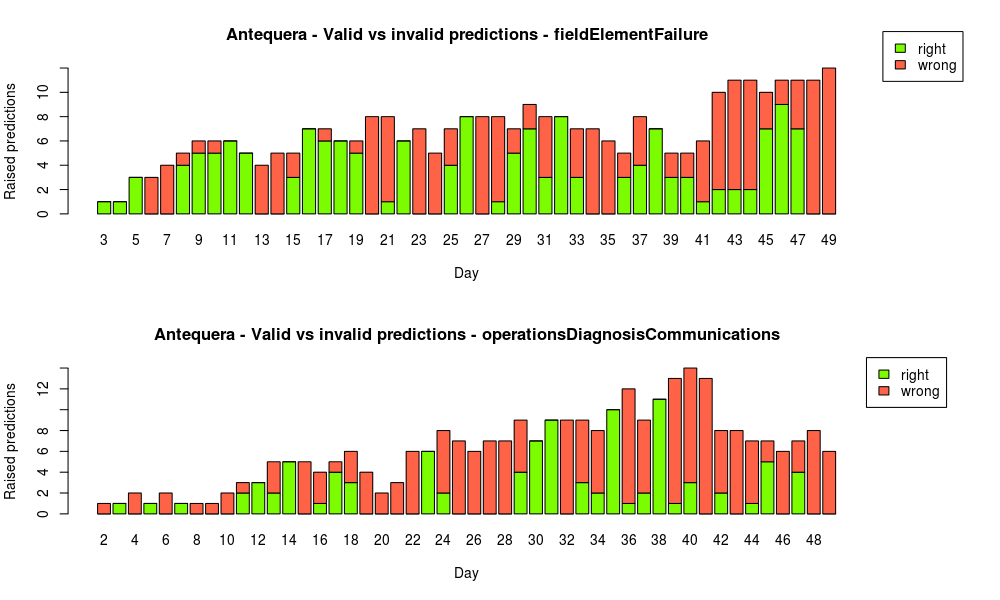
\includegraphics[width=\textwidth]{img/scenario_right_wrong.png}
\caption{Timeline of predictions during a sample period} \label{fig:scenario_right_wrong}
\end{figure}

\begin{figure}[hbtp]
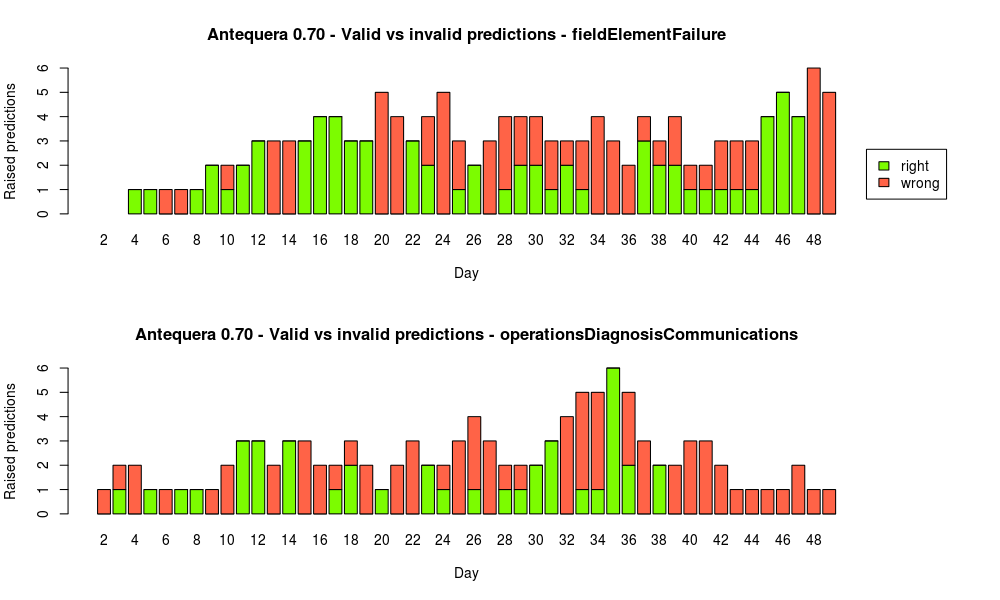
\includegraphics[width=\textwidth]{img/scenario_right_wrong_70.png}
\caption{Timeline of predictions during a sample period} \label{fig:scenario_right_wrong_70}
\end{figure}

\begin{figure}[hbtp]
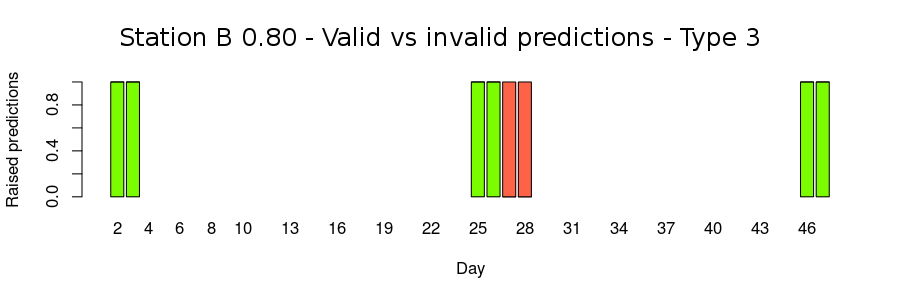
\includegraphics[width=\textwidth]{img/scenario_right_wrong_80.png}
\caption{Timeline of predictions during a sample period} \label{fig:scenario_right_wrong_80}
\end{figure}

\clearpage

\section{Conclusions}
The results obtained after the development of the presented procedures are found to be satisfactory, as shown in section~\ref{sec:desc_results}. Large rule sets with high precision values have been found for several stations and different time windows.

For this rulesets to be useful for Thales' operators, a implementation of a rule engine is necessary. This aspect with be covered in next stages of the project, and it is completely independent from the procedures described in this document which were used to obtain the predictive knowledge.

Also, results have been found to vary significantly in terms of quantity and precision in different stations and time periods, as seen in section~\ref{sec:desc_results}. In order to obtain higher quality results, it is necessary to explore alternative methods which can get over the limitations found with the performed method. First of all, the used algorithms can be vastly optimised to perform much better in our specific scenario. When searching for frequent sequences, we cannot limit the number of terms in the \emph{consequent}, as the maximum number of terms in each member of the sequence is fixed by a single parameter. In our case, we do not want to use sequences with more than one element in the consequent (as explained in section~\ref{sec:rule_model}) but our algorithm is still generating them as sequence candidates. This increases the complexity of the algorithm significantly, as we are growing our candidates in both the antecedent and the consequent of the rule while we only need the antecedent to grow.

Furthermore, as mentioned in section~\ref{sec:rule_model}, the candidates for rules are selected amongst sequences which are \emph{frequent}. Although this provides a good starting point in order to find predictive rules, we must perform two kinds of filtering in order to obtain the final rule sets: first by frequency, and later by precision. A new algorithm could be implemented in the same fashion as cSPADE, but performing only a filtering in terms of precision. This would not only save time and allow deeper searches, but also avoid disregarding those sequences which are not frequent but might lead to precise predictions.

Additionally, as seen in section~\ref{sec:datamining}, there are many other types of data mining algorithms which could be used or adapted to our problem. Specifically, a parallell approach has been made using \emph{Bayesian Networks}. These networks provide a very useful mathematical model which can be used to predict information in a similar fashion than the rules. However, it usually requires a deep previous knowledge on the events of the system and their possible relations in order to obtain their full potential. After building some of these models and obtaining said information from Thales' engineers, the model based on \emph{association rules} was still found to perform much better in all terms. Additional research would be necessary in order to obtain better results with these alternative tools.

Finally, we have found that one of the best and most immediate ways to increase the quality of the results is to divide the large datasets into smaller clusters. In section~\ref{sec:dataclustering} we have presented two possible clustering methods which have indeed improved the results significantly. Further improvement could be achieved by performing a deeper research on alternative clustering methods. Specifically, the method described in section~\ref{sec:group_elements} was found to increase peformance in very high rates. Developing a way to make this clustering method automatisable and directly feasible for all the stations would likely highly increase performance.

Summarising, in order to obtain higher quality results, a way must be found to face limits in terms of computation capabilities. The server available for our project is powerful enough as to think of improving hardware. Therefore, software and data optimisation is the only way to obtain significant improvement in the results.

\clearpage

\chapter{Chapter 4}

\section{Module description}
\label{sec:module_description}
In this section we will provide a general description of the implemented prototype. This prototype allows the usage of already existing association rules, which have been already obtained as the result of a \emph{Data Mining}\cite{torgo2003data}\cite{han2006data} procedure. These rules do not offer any functionality by themselves, as a system is needed to check whether their conditions are fulfilled and therefore a prediction can be made.

Rules are simply textual information in the form of "When A and B happen together, C has 80\% chances of happening". This information would be useful for an operator who might be manually checking events and would be able to expect C after seeing A and B. However, real systems usually have a much larger set of possible events, and many more events happening during each observation, and therefore an automated system is needed to perform these operations.

We call such a system a \emph{Rule engine}\cite{liang2009openrulebench}. A rule engine is simply a system which evaluates input conditions and fires the rules which comply with these conditions, outputting the result of said rules. In our case, the system will take as input a set of current events, and output a list of predictions along with their probabilities.

The implementation of a rule engine is not a trivial matter, and requires a significant amount of work to achieve optimal results in terms of computation requirements and complexity. Therefore, we will count on one of the already existing solutions which suits our needs perfectly and in a very optimised way: the JBoss Drools Expert library\cite{browne2009jboss}. This library is freely available as a java module and counts on several interoperability options, which makes it perfect for the usage in our project. The only requirement this imposes is the need of translating our rules to a Drools-compatible format, a matter which will be addressed later on this document.

\subsection{Parameters and interfaces}
\label{sec:parameters_and_interfaces}
Depending on our needs for each situation, our system can obtain predictions for several periods of time, different types of systems and different input lengths. Specifically, we count on rules for four different stations of different characteristics (Albacete, Antequera, Segovia and Sevilla) and for three different time windows (one day, two days and seven days). Each of these prediction modes needs a different type of input and needs to use a different set of rules. This distinction has therefore been made at the time of generating the rules, and now those rules need to be loaded accordingly to the kind of prediction we want to obtain.

In other words, said parameters (station type and time window) fixes the set of rules to be used and the length of the input to be provided. This association also works in the other direction: by using an specific rule set and an specific input, we are already defining the execution parameters. Therefore, both the station type and prediction time window are irrelevant for the correct function of our predictive module. It is responsibility of the operator or executing system to select the appropriate rule set and provide an appropriate input. This allows new execution options to be added or updated at any time, without the need of modifying the module in any way. If we generate a new set of rules expecting a whole month of input and which will generate a month of predictions, we just need to load it and know what it is generating. Also, if we generate rules for a new type of maintenance station we just need to load them on the module and provide an input according to that new type of station.

The architecture of the module is very simple. It counts on an Engine class which streamlines the whole procedure, relying on three model classes to provide Alarm and prediction representations. A class diagram can be seen in figure~\ref{fig:prototypeArchitecture}

\begin{figure}[hbtp]
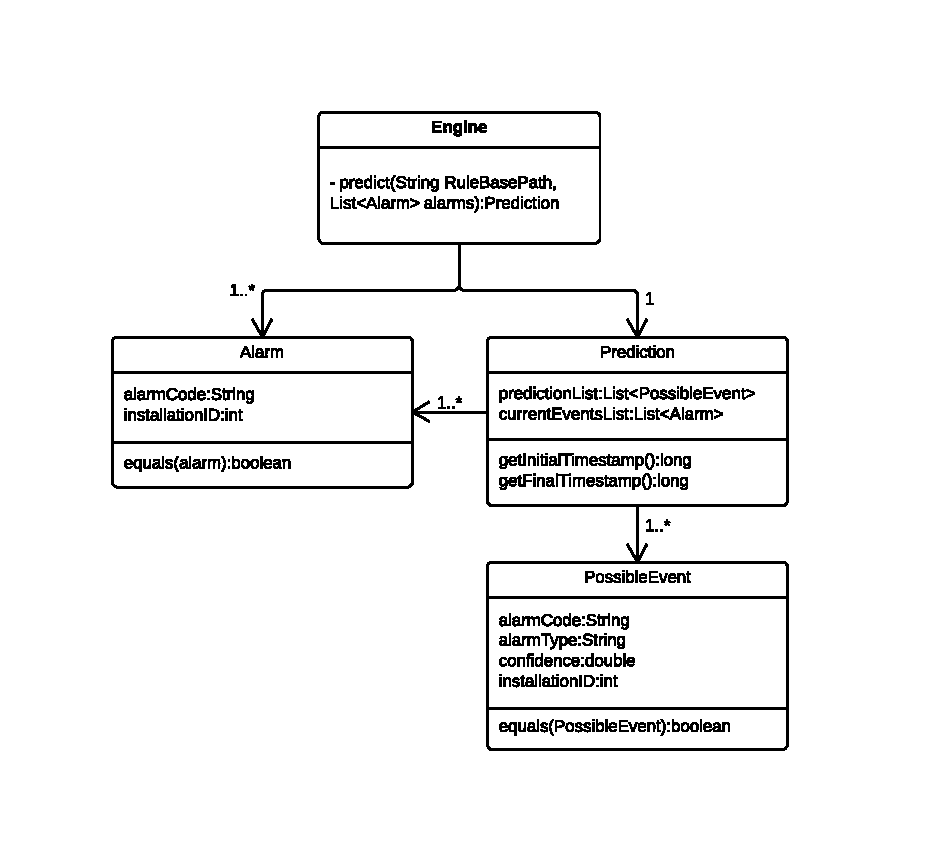
\includegraphics[width=\textwidth]{img/prototypeArchitecture.pdf}
\caption{Class diagram for the implemented module} \label{fig:prototypeArchitecture}
\end{figure}

\subsection{Input selection and execution}
As described in section~\ref{sec:parameters_and_interfaces}, our module takes a list of Alarm objects and outputs a Prediction object containing a list of PossibleEvent objects. We have also seen that it is important to provide an input which adequates to the conditions imposed by the selected rule set (or viceversa), which simply means that we must provide a list containing an observation time whose length adequates to that expected by the rule set.

Furthermore, as seen in figure~\ref{fig:prototypeArchitecture}, Alarms are described not only by their alarm code, but also by the installation in which they have been raised. It is important to have into account that alarms are only related to others happening in the same installation, and therefore we only need inputs to contain sets which are complete in terms of installation id. In other words, we could call the inference engine with separated inputs containing each the alarms which have been raised by each of the installations. However, as the rule sets are the same for all of the installations under the same maintenance station, it is more efficient to make this distinction during execution instead of having to call the engine and load the rules several times.

\subsection{The rule engine}
In section~\ref{sec:module_description} we introduced the concept of \emph{the rule engine}, the core of our module in which most of the heavy processing happens. Amongst all the available solutions, we selected the \emph{Drools Expert}\cite{browne2009jboss} platform, as it is the most advanced solution available for Java environments, and therefore an easy integration can be made with the rest of the maintenance station software.

\emph{Drools Expert} relies on \emph{Drools rule files}, which are plain text files containing our rules coded with an special syntax. Furthermore, it provides several ways of managing and even changing these rules, as interfaces for business users or other tools to easily generate these files based on workflow diagrams or other sources. However, as the knowledge on which our rules are based is obtained from a different source (a fully independent Data Mining process) we won't make use of these posibilities and will just have to consider the output format for our rules, to make it directly compatible with Drools' syntax. In section~\ref{sec:description_of_rule_sets} we will provide further description of these rule sets, as well as their generation and conversion processes.

Our module encapsulates and streamlines the execution of Drools Expert and their preparation process. The details of this configuration are of little relevance, and can be summarized as \emph{choosing a rule set} and \emph{provide a valid input}. Our module will then simply evaluate all the rules and then provide an output with a prediction for the next period, as we described in section~\ref{sec:parameters_and_interfaces}. The cornerstone of all this process is therefore the rule set. As we will describe in section~\ref{sec:description_of_rule_sets}, it is of essential importance to carefully build these in order to obtain a proper function of the rule engine. In the end, the rules are actually part of the code of our module, on which reiles most of its functionality.

A sequence diagram of the module's function can be seen in figure~\ref{fig:prototypeSequence}

\begin{figure}[hbtp]
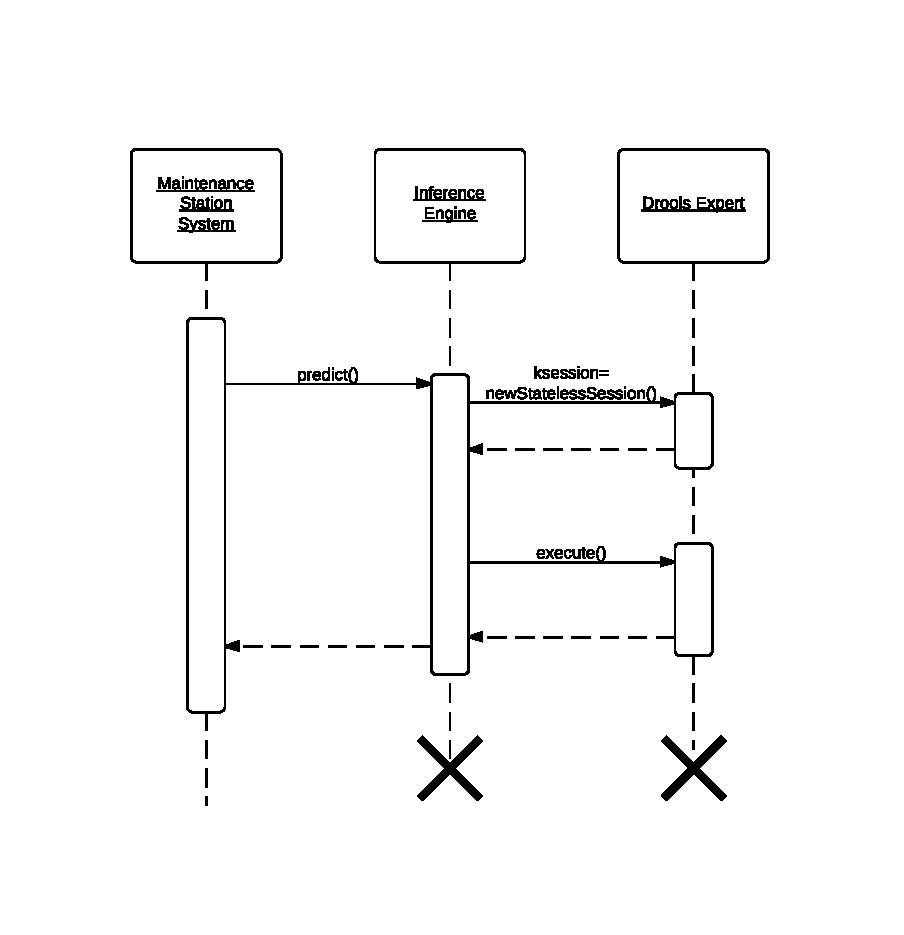
\includegraphics[width=\textwidth]{img/prototypeSequence.pdf}
\caption{Sequence diagram for the implemented module} \label{fig:prototypeSequence}
\end{figure}

\section{Description of rule sets}
\label{sec:description_of_rule_sets}
In this section we are going to describe the most important part of our prediction module: the rule sets. A rule set is simply a plain text file containing the necessary information for a rule to be evaluated and fired in the adequate circumstances. A rule can be simply seen as a piece of information stating that "When \emph{A} and \emph{B} happen, \emph{C} will happen with a certainty of 80\%", but there is actually a few more compexity added for the proper functioning of our system.

First of all, as we mentioned in section~\ref{sec:parameters_and_interfaces}, we have to take into account that events have to happen in the same installation for alarms to be raised. In other words, the rule above would be actually needed to be stated as follows:

\emph{"When A happens, and B happens in the same installation as A, C will happen in the same installation with a certainty of 80\%"}

Also, although it is not necessary for the basic function of our module, we will also return the type of alarm we are predicting in the output. The type of alarm can be directly inferred from the alarm code itself, but as we are working with hardcoded rulesets which only need to be generated once, it is much more efficient to associate the alarm type with each rule than having to perform a search every time an event is predicted. This does not affect how or module works at all, but our rule will actually look more like:

\emph{"When A happens, and B happens in the same installation as A, C (Which is an event of type 1) will happen in the same installation with a certainty of 80\%"}

This information can be useful to provide an overview of the kind of systems which are more prone to fail in a short future, and probably assign resources to groups instead of actual specific events for organisational convenience.

It is important to note that we are not mentioning at all time periods either for the observation (events A and B) or the expectation (event C). As we mentioned in section~\ref{sec:parameters_and_interfaces}, those parameters are implicit to the whole set of rules. For example, we \emph{know} we are talking of an observation of one day and a prediction for one day in the future because we are loading the ruleset whose rules work with that time windows. This is much more convenient as reduces the complexity of the rules avoiding having to handle additional parameters, but needs that the calling process takes into account these parameters by itself.

The same applies for the type of station we are working with. Even though the stations we are working with are quite different from each other, we do not specify in the rules where do we expect those events to hapen. Or we don't specify that \emph{explicitly}, because again, each rule set works exclusively for one specific station.

There is also a third parameter which we can directly affect simply by selecting an specific rule set: confidence. Instead of having to filter rules by their confidence when setting a threshold, it is much more efficient and convenient to load only those rules which provide predicitons with a confidence higher than a given threshold. As we mentioned, rulesets are plain text files which contain all the rules to be loaded, so by simply removing those with low confidence, we can perform this filtering in a very efficient way.

It is up to the maintenance operator to decide upon these thresholds. In order to be on the safe side, we usually set a threshold of 50\% (which is, predictions which are more likely to be right than wrong), but for an operator it might be more convenient to disregard maybe even predictions whose confidence are lower than 70\% or 80\%. By directly removing those rules from the rule sets, the additional computation needed to evaluate them is eliminated, and therefore the execution would be much more efficient.

The specific list of sets which have been generated and provided can be seen in table~\ref{tab:ruleset_list}.

\begin{table}
\begin{center}
\begin{tabular}{|c|c|c|c|c|}
\hline \headcell{Rule set} & \headcell{Station} & \headcell{Observation} & \headcell{Prediction} & \headcell{Min. Confidence} \\ 
\hline 
albacete1d\_70.drl & Albacete & 1 day & next day & 70\% \\ 
\hline  
albacete7d\_70.drl & Albacete & 7 days & next 7 days & 70\% \\ 
\hline 
antequera1d\_70.drl & Antequera & 1 day & next day & 70\% \\ 
\hline 
segovia1d\_70.drl & Segovia & 1 day & next day & 70\% \\ 
\hline
segovia2d\_70.drl & Segovia & 2 days & next 2 days & 70\% \\  
\hline 
segovia7d\_70.drl & Segovia & 7 days & next 7 days & 70\% \\  
\hline 
sevilla1d\_70.drl & Sevilla & 1 day & next day & 70\% \\ 
\hline
albacete1d\_50.drl & Albacete & 1 day & next day & 50\% \\ 
\hline 
albacete7d\_50.drl & Albacete & 7 days & next 7 days & 50\% \\ 
\hline 
antequera1d\_50.drl & Antequera & 1 day & next day & 50\% \\ 
\hline 
segovia1d\_50.drl & Segovia & 1 day & next day & 50\% \\ 
\hline
segovia2d\_50.drl & Segovia & 2 days & next 2 days & 50\% \\  
\hline 
segovia7d\_50.drl & Segovia & 7 days & next 7 days & 50\% \\  
\hline 
sevilla1d\_50.drl & Sevilla & 1 day & next day & 50\% \\ 
\hline
albacete1d\_all.drl & Albacete & 1 day & next day & -- \\ 
\hline  
albacete7d\_all.drl & Albacete & 7 days & next 7 days & -- \\ 
\hline 
antequera1d\_all.drl & Antequera & 1 day & next day & -- \\ 
\hline 
segovia1d\_all.drl & Segovia & 1 day & next day & -- \\ 
\hline
segovia2d\_all.drl & Segovia & 2 days & next 2 days & -- \\  
\hline 
segovia7d\_all.drl & Segovia & 7 days & next 7 days & -- \\  
\hline 
sevilla1d\_all.drl & Sevilla & 1 day & next day & -- \\ 
\hline

\end{tabular} 
\caption{Generated rule sets} \label{tab:ruleset_list}
\end{center}
\end{table}

\subsection{Generation of rule sets}
\label{sec:generation_of_rule_sets}

We have mentioned in section~\ref{sec:module_description} that our rules are obtained through a \emph{Data Mining process}, and later translated into the Drools syntax. In this section we are going to give an overview of the whole process.

Everything starts with a database backup provided by Thales' engineers which contains a large amount of event logs in all the stations we are going to study. That database is transformed into a working set, a process which involves several processes such as variable reduction, data normalisation and format conversion. This data is loaded into an R\cite{ihaka1996r, torgo2003data} environment in which the core data mining procedure is performed: the rule discovery process. This step forms the core of the whole procedure, and requires a considerable amount of resources and time.

This generates a raw list of association rules, in the format of R data frames. At this point we can already perform some filtering to separate the useful rules from those with very low confidence values. However, as those rules can also be useful for future research or to be manually analysed by maintenance operators, so far we have decided to save the whole amount of generated rules whichever their precision was.

A last process is performed in which we convert the raw R data frames\cite{ihaka1996r} containing the rules into the Drools syntax. At this point we also generate several subsets with different confidence thresholds, as mentioned in section~\ref{sec:description_of_rule_sets}. This step is fully automated with Python\cite{sanner1999python} scripts. An example of both formats will be shown in section~\ref{sec:structure_of_rules_and_sets}.

A diagram of the whole process can be seen in figure~\ref{fig:prototypeGenProcess}.

\begin{figure}[hbtp]
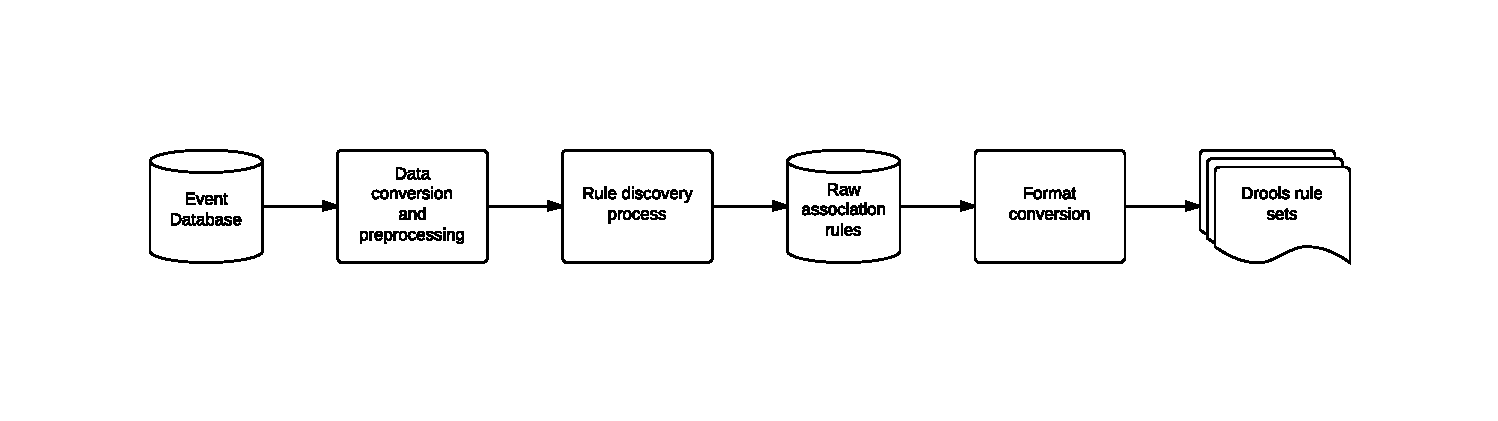
\includegraphics[width=\textwidth]{img/prototypeGenProcess.pdf}
\caption{The whole rule generation process} \label{fig:prototypeGenProcess}
\end{figure}

\subsection{Structure of rules and sets}
\label{sec:structure_of_rules_and_sets}
In this section we will now analyse the actual structure of our rules and their conversion to the Drools syntax. We will take the following rule as an illustrating example:

\begin{minted}[mathescape,
               linenos,
               numbersep=5pt,
               gobble=0,
               frame=lines,
               framesep=2mm]{java}
"<{
	saml.status.energy_net1_not_present
	saml.status.energy_net2_not_present
	saml.status.energy_48V_battery_nok
	saml.status.energy_SAI_PT_nok
},{
	saml.status.energy_SAI_ST_nok
}>",
0.83833333,
0.089034423
\end{minted}

That is the appearance of a prediction rule in the format of R data frame. Lines 2, 3 and 4 are the antecedents, line 6 is the predicted event and rule 8 is the precision of the rule. The last number on line 9 is the recall of the rule, an evaluation value which is of no use at this moment.

The same rule in Drools syntax would looks as follows:

\begin{minted}[mathescape,
               linenos,
               numbersep=5pt,
               gobble=0,
               frame=lines,
               framesep=2mm]{java}
rule "rule0"
    when 
        Alarm(iid : installationID, alarmCode 
        		== "saml.status.energy_net1_not_present");
        Alarm(installationID == iid, alarmCode 
        		== "saml.status.energy_net2_not_present");
        Alarm(installationID == iid, alarmCode 
        		== "saml.status.energy_48V_battery_nok");
        Alarm(installationID == iid, alarmCode 
        		== "saml.status.energy_SAI_PT_nok");
    then 
        PossibleEvent p = new 
        	PossibleEvent("saml.status.energy_SAI_ST_nok",
        			"fieldElementFailure",iid,0.83833333);
        resultList.add(p);
end
\end{minted}

We can see here the additions mentioned in section~\ref{sec:description_of_rule_sets}, regarding installation code and event type (which is hardcoded here to "filedElementFailure"). The resultList object conforms the output which will be returned by Drools to our module, containing all the generated possible events.

\section{Output visualisation}
When describing our predictive module, we haven't so far spoken on how this data is visualised or shown to maintenance operators. This is because our module does not provide a visual interface in any way to make this data user-readable. The predictive module is meant to be integrated in a much larger system which is Thales' railway maintenance station software. This will provide operators a visualization of the predictions, and can even provide means for automatic prediction handling.

However, in order to illustrate the possibilities offered by the implemented prototype, we have developed a demonstration interface. This illustrative example can be seen in figure~\ref{fig:demoExample}.

\begin{figure}[hbtp]
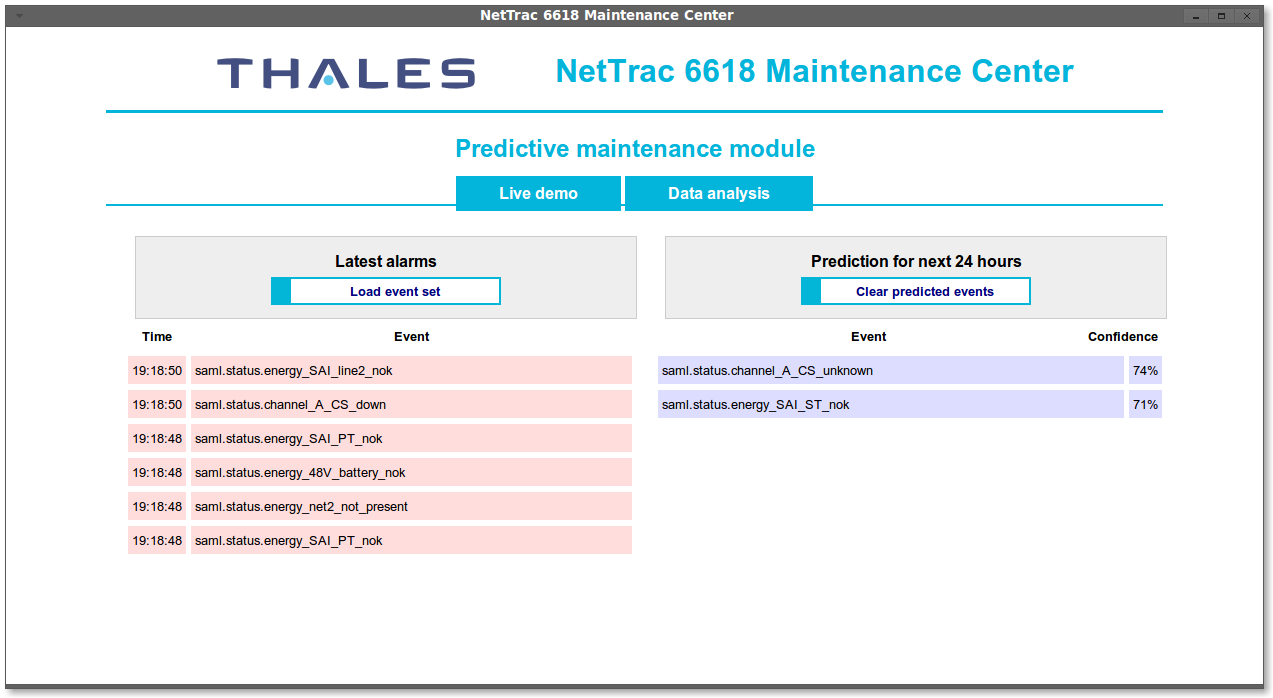
\includegraphics[width=\textwidth]{img/demoExample.png}
\caption{Example demo interface} \label{fig:demoExample}
\end{figure}

\clearpage

\section{Conclusions}
At this stage of the project, we have already developed a fully functional predictive module to be integrated within Thales' maintenance station. Furthermore, a demo interface has been provided in order to illustrate one of the multiples applications this module can offer to maintenance operators.

However, the module allows Thales' engineers to perform much more advanced tasks with these predictive information. From statistical reports including information on the predictions, to automatic processes started as response to specific predicted events, the range of possibilities is quite large.

Integration is also possible within any other kind of system, due to the implementation of the module as a Java library. Furthermore, it is even possible to build a standalone predictive system, performing predictions sobre already generated static event sets.

In general terms, the implementation of the module has been successful and completely fulfils our goals.

\clearpage



\bibliographystyle{plain} 
\bibliography{datamining}

\end{document}